%%%%%%%%%%%%%%%%%%%%%%%%%%%%%%%%%%%%%%%%%
% Masters/Doctoral Thesis 
% LaTeX Template
% Version 2.5 (27/8/17)
%
% This template was downloaded from:
% http://www.LaTeXTemplates.com
%
% Version 2.x major modifications by:
% Vel (vel@latextemplates.com)
%
% This template is based on a template by:
% Steve Gunn (http://users.ecs.soton.ac.uk/srg/softwaretools/document/templates/)
% Sunil Patel (http://www.sunilpatel.co.uk/thesis-template/)
%
% Template license:
% CC BY-NC-SA 3.0 (http://creativecommons.org/licenses/by-nc-sa/3.0/)
%
%%%%%%%%%%%%%%%%%%%%%%%%%%%%%%%%%%%%%%%%%

%----------------------------------------------------------------------------------------
%	PACKAGES AND OTHER DOCUMENT CONFIGURATIONS
%----------------------------------------------------------------------------------------

\documentclass[
11pt, % The default document font size, options: 10pt, 11pt, 12pt
oneside, % Two side (alternating margins) for binding by default, uncomment to switch to one side
english, % ngerman for German
singlespacing, % Single line spacing, alternatives: onehalfspacing or doublespacing
%draft, % Uncomment to enable draft mode (no pictures, no links, overfull hboxes indicated)
%nolistspacing, % If the document is onehalfspacing or doublespacing, uncomment this to set spacing in lists to single
%liststotoc, % Uncomment to add the list of figures/tables/etc to the table of contents
%toctotoc, % Uncomment to add the main table of contents to the table of contents
%parskip, % Uncomment to add space between paragraphs
%nohyperref, % Uncomment to not load the hyperref package
headsepline, % Uncomment to get a line under the header
%chapterinoneline, % Uncomment to place the chapter title next to the number on one line
%consistentlayout, % Uncomment to change the layout of the declaration, abstract and acknowledgements pages to match the default layout
]{MastersDoctoralThesis} % The class file specifying the document structure

\usepackage[utf8]{inputenc} % Required for inputting international characters
\usepackage[T1]{fontenc} % Output font encoding for international characters

\usepackage{mathpazo} % Use the Palatino font by default

\usepackage[backend=bibtex,style=authoryear,natbib=true,maxcitenames=2,mincitenames=1]{biblatex}

\addbibresource{references.bib} % The filename of the bibliography

\usepackage[autostyle=true]{csquotes} % Required to generate language-dependent quotes in the bibliography

\usepackage{tikz}

\usepackage{tabularx}
\usepackage{booktabs}
\usepackage{multirow}
\usepackage{enumitem}
\usepackage{soul}
\usepackage{booktabs}
\usepackage{array}
\usepackage{amssymb}
\usepackage{amsmath}
\usepackage{multicol}
\usepackage{graphicx}
\usepackage{array}
\usepackage[table]{xcolor}
\usepackage{makecell}
\usepackage{float}

\usepackage{etoolbox}

\makeatletter
\patchcmd{\l@chapter}{\vskip 1.0em}{\vskip 0.3em}{}{}
\makeatother

% Align List of Figures and List of Tables entries with the left margin
\makeatletter
\renewcommand*\l@figure{\@dottedtocline{1}{0em}{3em}}
\renewcommand*\l@table{\@dottedtocline{1}{0em}{3em}}
\makeatother


%----------------------------------------------------------------------------------------
%	MARGIN SETTINGS
%----------------------------------------------------------------------------------------

\geometry{
	paper=a4paper, % Change to letterpaper for US letter
	inner=2.5cm, % Inner margin
	outer=2.5cm, % Outer margin
	bindingoffset=.5cm, % Binding offset
	top=2.5cm, % Top margin
	bottom=2.5cm, % Bottom margin
	%showframe, % Uncomment to show how the type block is set on the page
}

%----------------------------------------------------------------------------------------
%	THESIS INFORMATION
%----------------------------------------------------------------------------------------

\thesistitle[Environmental Footprints of Financial Systems: US and EA]{Environmental Footprints of Financial Systems: The United States and The Euro Area}
\supervisor{Prof. Eric \textsc{Jondeau}} % Your supervisor's name, this is used in the title page, print it elsewhere with \supname
\examiner{} % Your examiner's name, this is not currently used anywhere in the template, print it elsewhere with \examname
\author{Hoai-Thuong \textsc{Phan}} % Your name, this is used in the title page and abstract, print it elsewhere with \authorname
\addresses{} % Your address, this is not currently used anywhere in the template, print it elsewhere with \addressname

\subject{} % Your subject area, this is not currently used anywhere in the template, print it elsewhere with \subjectname
\keywords{ESG} % Keywords for your thesis, this is not currently used anywhere in the template, print it elsewhere with \keywordnames
\university{{University of Lausanne}} % Your university's name and URL, this is used in the title page and abstract, print it elsewhere with \univname
\department{\href{http://department.university.com}{Department or School Name}} % Your department's name and URL, this is used in the title page and abstract, print it elsewhere with \deptname
\group{\href{http://researchgroup.university.com}{Research Group Name}} % Your research group's name and URL, this is used in the title page, print it elsewhere with \groupname
\faculty{\href{http://faculty.university.com}{Faculty Name}} % Your faculty's name and URL, this is used in the title page and abstract, print it elsewhere with \facname

\AtBeginDocument{
\hypersetup{pdftitle=\ttitle} % Set the PDF's title to your title
\hypersetup{pdfauthor=\authorname} % Set the PDF's author to your name
\hypersetup{pdfkeywords=\keywordnames} % Set the PDF's keywords to your keywords
}


\makeatletter
\setlength{\@fptop}{0pt} % Forces float pages to align to the top rather than center
\setlength{\@fpbot}{0pt plus 1fil}
\makeatother

\begin{document}

% \frontmatter % Commented out so page numbers don't switch to Roman numerals
\pagestyle{scrheadings} % Enforces our new custom headers/footers

%----------------------------------------------------------------------------------------
%	TITLE PAGE
%----------------------------------------------------------------------------------------

\begin{titlepage}

\begin{center}

\vspace*{.06\textheight}
{\scshape\LARGE \univname\par}\vspace{1.5cm} % University name
\textsc{\Large Master's Thesis}\\[0.5cm] % Thesis type

\HRule \\[0.4cm] % Horizontal line
{\huge \bfseries \ttitle\par}\vspace{0.4cm} % Thesis title
\HRule \\[1.5cm] % Horizontal line
 
\begin{minipage}[t]{0.4\textwidth}
\begin{flushleft} \large
\emph{Author:}\\
{\authorname} % Author name - remove the \href bracket to remove the link
\end{flushleft}
\end{minipage}
\begin{minipage}[t]{0.4\textwidth}
\begin{flushright} \large
\emph{Supervisor:} \\
{\supname} % Supervisor name - remove the \href bracket to remove the link  
\end{flushright}
\end{minipage}\\[1cm]


% Absolute positioning to override margins
\begin{tikzpicture}[remember picture,overlay]
    \node[anchor=south east, xshift=-1.5cm, yshift=1.5cm] at (current page.south east) {
        
\includegraphics[scale=0.15]{Figures/UNIL-LOGOTYPE-BLUE-CMYK.eps}
    };
\end{tikzpicture}

\end{center}
\end{titlepage}

%----------------------------------------------------------------------------------------
%	ABSTRACT PAGE
%----------------------------------------------------------------------------------------

\clearpage
\thispagestyle{empty} % Ensures the page is unnumbered per the guidelines

\begin{center}
    \LARGE \textbf{Abstract}
\end{center}
\vspace{1cm}

This thesis applies a macroeconomic framework that combines national financial accounts with an environmentally extended multi-regional input-output (EE-MRIO) model to quantify the greenhouse gas (GHG) emissions and broader environmental pressures financed by the United States and the Euro area. Overall, financed emissions in both financial systems declined after peaking in 2008, but the results reveal a marked structural divergence. The US market-based financial system remains predominantly domestically oriented, with all financial groups contributing to the financing of domestic emitters. By contrast, the Euro area’s bank-based financial system exhibits a growing cross-border footprint, with foreign claims accounting for approximately 40\% of its total portfolio in 2022.

Under the assumption that outbound funds are directed to both developed and emerging markets, the Euro area’s total financed emissions exceed those of the United States in recent years, reaching 4,082.38 MtCO$_2$e in 2022, compared with 3,761.45 MtCO$_2$e for the United States. This scale is close to the Euro area’s production- and consumption-based footprints, suggesting that financial exposures abroad represent a major channel through which the region’s environmental footprint extends beyond its borders. Beyond GHG emissions, the results also show that financial institutions in the Euro area are also associated with substantial land use, water consumption, and resource extraction outside the region. 



\vspace{1.5cm}

\noindent \textbf{Keywords:} ESG, National financial accounts, Financed emissions, Input-output analysis, Climate-related risks \\
\textbf{JEL Classification:} G20, Q54, Q56, E44, C67

\cleardoublepage





%----------------------------------------------------------------------------------------
%	ACKNOWLEDGEMENTS
%----------------------------------------------------------------------------------------

\begin{acknowledgements}
\addchaptertocentry{\acknowledgementname} % Add the acknowledgements to the table of contents
I would like to express my gratitude to Professor Eric Jondeau for his input and advice throughout the writing of this thesis, and also for his kind support during my  academic journey. 

My master's journey is also dedicated to my parents for their strong belief in the value of education, to my sister for her unconditional support in whichever path I choose to take in life, and to my niece and nephew for their mere presence with cuteness.

I am also thankful to friends I have encountered in Lausanne, who have broadened my horizons and enriched my perspectives in many ways: Angelique, Gabriele, Dimitar, Carlo, Ashley, Fredrik, and friends who are very far away yet have been always very dear to me: Andres, Tran, Hung, Giang-Tu, Y-Phan, Bich-Thao.

And finally I thank myself for walking through difficulties with courage and for  holding on to a belief in the good things in life.
\end{acknowledgements}

%----------------------------------------------------------------------------------------
%	LIST OF CONTENTS/FIGURES/TABLES PAGES
%----------------------------------------------------------------------------------------

\tableofcontents % Prints the main table of contents

\begingroup
\makeatletter
\let\oldaddvspace\addvspace
\renewcommand*\addvspace[1]{}
\listoftables
\listoffigures
\let\addvspace\oldaddvspace
\makeatother
\endgroup
%----------------------------------------------------------------------------------------
%	ABBREVIATIONS
%----------------------------------------------------------------------------------------


\begin{abbreviations}{@{}ll@{}}

\noindent

BCBS    & Basel Committee on Banking Supervision \\
CBA     & Consumption-based accounting\\
DIS     & Discrepancy sector\\
ECB     & European Central Bank\\
ESA     & The European System of National Accounts \\
ESRB    & European Systemic Risk Board \\
EU      & European Union\\
EZ      & Eurozone \\
FWTW    & From-whom-to-whom\\
GG      & General government\\
GHG     & Greenhouse Gas\\
HH      & Household and nonprofit organizations\\
IMF     & International Monetary Fund\\
IPFP    & Iterative Proportional Fitting Procedure\\
IS      & Insurance Corporations\\
MFI     & Monetary Financial Institutions\\
MRIO    & Multi-regional Input-output model\\
NFC     & Non-financial business\\
NGFS    & Network for Greening the Financial System \\
NM\_MFIF & Non-money Market Funds Investment Funds\\
NPISH   & Non-profit institutions serving households\\
OFI     & Other Financial Institutions\\
PBA     & Production-based accounting\\
PBC     & The People's Bank of China\\
PCAF    & The Partnership for Carbon Accounting Financials\\
PEN     & Pension Funds\\
RoW     & Rest of the world\\
SDR     & Special Drawing Right\\
SNA     & System of National Accounts \\



\end{abbreviations}


%----------------------------------------------------------------------------------------
%	THESIS CONTENT - CHAPTERS
%----------------------------------------------------------------------------------------
% \mainmatter % Commented out so the page count doesn't reset to 1
\pagestyle{scrheadings} % Enforces our new custom headers/footers

% Include the chapters of the thesis as separate files from the Chapters folder
% Uncomment the lines as you write the chapters

% Chapter 1

\chapter{Introduction} % Main chapter title

\label{Chapter1} % For referencing the chapter elsewhere, use \ref{Chapter1} 

%----------------------------------------------------------------------------------------

While financial institutions generate limited environmental impacts through their direct operations (such as office energy use and IT operations), they are indirectly responsible for substantial greenhouse gas (GHG) emissions by financing high-emitting firms. These are commonly referred to as “financed emissions” and are classified under Scope 3, Category 15 (“Investments”) downstream emissions \citep{ghg_protocol_corporate_2011}.

The relevance of financed emissions begins with the growing recognition that climate change can be a source of financial instability \citep{bolton_green_2020, esrb_esrb_2021}. Climate change may generate physical risks, arising from severe climate-related damages, and transition risks, arising from potentially disorderly mitigation strategies, regulatory changes, carbon pricing, technological change, or shifts in market expectations. At the portfolio level, measuring financed emissions allows financial institutions to assess their exposure to these risks through the companies they finance.

Moving from the portfolio level to the macroeconomic level, the same logic can be extended to the financial system as a whole. If domestic financial institutions are highly exposed to emissions-intensive sectors, financed emissions may become a source of systemic vulnerability. In this sense, the financed emissions of a country’s financial system can provide an indication of broader macro-financial risks. 

In an effort to establish a transparent and harmonized framework for disclosing financed emissions, the Partnership for Carbon Accounting Financials (PCAF) has developed the \textit{Global GHG Accounting and Reporting Standard for the Financial Industry}. While this standard has become widely adopted for attributing emissions at the asset and portfolio levels, its approach suffers from several inherent limitations \citep{pcaf_global_2022}. First, high-quality data remain scarce for certain asset classes, forcing institutions to rely on estimates or proxies. Second, pervasive double counting can occur, whether across different institutions, across asset classes, or when multiple lenders co-finance a single entity. Consequently, bottom-up financed emissions cannot be reliably aggregated to estimate a nation's total financial footprint. 

Beyond its contribution to GHG emissions, the financial system also contributes to broader environmental degradation by financing activities associated with intensive land use, water consumption, and resource extraction. Assessing these wider environmental pressures provides a more comprehensive view of the financial system’s role in climate change and environmental sustainability, thereby supporting the development of more robust sustainability metrics and policy responses. At the same time, the financial system is exposed to climate- and environment-related risks through investment portfolios that finance activities linked to environmental harm.

Building on the macroeconomic framework developed by \textcite{jondeau_environmental_2026}, this thesis quantifies the environmental footprint of two major financial centers: the United States and the Eurozone. The methodology relies on EXIOBASE, an \textit{environmentally extended multi-regional input-output} (EE-MRIO) database that provides GHG emissions, land use, water use, and material extraction at the country-industry level. By integrating these environmental extensions with macro-financial data, the framework attributes environmental pressures to specific groups of financial institutions based on their exposure to real-economy credit recipients. A primary challenge in this attribution is the complexity of financial intermediation chains, where institutions often lend to one another before capital reaches the real economy. Ignoring these intermediation links may lead to double counting or an incomplete measurement of financial exposures. To address this issue, the framework employs \textit{national financial accounts} alongside \textit{from-whom-to-whom} (FWTW) exposure networks. This makes it possible to trace environmental pressures generated by real-economy agents back to their ultimate financiers across the chain of financial intermediation.

The results reveal structural differences between the financial systems of the two regions, which in turn shape their exposure to climate- and nature-related risks. Banks have consistently remained the main source of financing in the Euro area, whereas the US financial system is more market-based, with several groups of financial institutions contributing to market financing. In terms of credit recipients, the US financial system primarily finances its domestic corporate sector. By contrast, Eurozone financial institutions have increasingly allocated funds to foreign counterparties over the past decade.

This shift has contributed to the Eurozone’s financed emissions surpassing those of the United States since 2016 onwards, under the assumption that outbound funds are directed to both developed and emerging markets. In 2022, GHG emissions attributed to the US financial system amounted to 3,761.45 million tonnes of CO\textsubscript{2}e, compared with 4,082.38 million tonnes of CO\textsubscript{2}e attributed to the Eurozone financial centre. This finding challenges the common perception that the Eurozone financial system is relatively green, a perception partly rooted in the European Union’s climate-policy leadership and extensive sustainable-finance regulatory framework, including the European Green Deal, the EU Emissions Trading System, the EU Taxonomy, and sustainable-finance disclosure rules \citep{merler_silvia_how_2025}. Despite this policy and regulatory leadership position, the results show that Eurozone financial institutions remain substantially exposed to emissions generated through their financing activities, particularly through cross-border exposures.

Compared with each region’s territorial and demand-driven emissions, financed emissions are relatively similar in magnitude in the Euro area, whereas in the United States they amount to only around half of these benchmarks. This contrast points to different channels through which emissions-reduction efforts may be prioritized. In the United States, reducing the carbon footprint of the financial system should be complemented by broader decarbonization across domestic industries. In the Euro area, by contrast, the decarbonization of financial portfolios appears especially important, as financed emissions constitute a substantial component of the region’s overall carbon footprint.


Beyond GHG emissions, the analysis also shows that financial-system-based accounting provides a distinct perspective on broader environmental pressures, including land use, water consumption, and resource extraction. These dimensions offer a more comprehensive view of the environmental footprint of financial systems and their exposure to nature-related risks.

The remainder of this thesis is organized as follows. Chapter 2 reviews the relevant literature. Chapters 3 and 4 introduce the conceptual framework and methodology, respectively. Chapter 5 describes the data used in the empirical analysis. Chapter 6 presents the results, and Chapter 7 concludes.
%----------------------------------------------------------------------------------------
% Chapter 2

\chapter{Literature Review} % Main chapter title

\label{Chapter2} % For referencing the chapter elsewhere, use \ref{Chapter2} 
%----------------------------------------------------------------------------------------
This chapter reviews three strands of literature relevant to this thesis: first, studies on the relationship between financial systems and environmental outcomes; second, research on climate- and nature-related financial risks; and third, work on financed emissions and financial-system environmental footprints.


The relationship between finance and the environment has received increasing attention in both academic and policy discussions. One strand of the literature examines how financial systems affect environmental outcomes through the allocation of capital across firms, sectors, and technologies. Financial institutions and markets influence which economic activities receive funding and under what conditions, and therefore may shape the emissions intensity of the economy. \textcite{kim_carbon_2020}, for example, show that financial development has a non-linear relationship with CO$_2$ emissions: financial deepening may initially increase emissions by expanding economic activity, but can eventually contribute to emissions reductions as capital is reallocated towards cleaner technologies and more efficient production. They also show that financial structure matters, as more competitive and less concentrated banking systems are associated with improvements in environmental quality over the longer term. Additionally, \textcite{ecb_finance_2019} examine the role of financial structure and find that CO$_2$ emissions per capita tend to be lower in economies that rely more heavily on equity financing. A possible mechanism is that stock markets facilitate the reallocation of capital towards less polluting sectors and place greater pressure on carbon-intensive firms to adopt cleaner technologies.

The relationship also works in the opposite direction: climate change and environmental degradation can create risks for financial institutions and financial stability. The literature commonly distinguishes between physical risks, arising from the direct impacts of climate change, and transition risks, arising from the adjustment to a low-carbon economy \citep{bolton_green_2020, ngfs_call_2019}. Physical risks may damage assets, disrupt production, and reduce borrowers' repayment capacity, while transition risks may arise from carbon pricing, environmental regulation, technological change, and shifts in investor or consumer preferences \citep{ecb_financial_2021}. These risks can affect banks through credit losses and investors through asset-price adjustments, as climate-related shocks are transmitted through both microeconomic and macroeconomic channels \citep{bcbs_climate-related_2021, ecb_financial_2021}. At the aggregate level, concentrated exposures to emissions-intensive or climate-vulnerable sectors may therefore become relevant for financial stability, especially when such exposures are interconnected across institutions and markets \citep{battiston_climate_2017, ecb_financial_2021}.

More recent literature extends this climate-finance perspective to biodiversity loss and nature-related financial risks. This literature emphasizes that financial institutions are exposed not only to firms with high GHG emissions, but also to firms and sectors that depend on ecosystem services or contribute to nature degradation. \textcite{kedward_biodiversity_2023} argue that biodiversity-related financial risks are closely connected to climate-related risks, but have received comparatively less attention from central banks and supervisors. Several studies have attempted to quantify the financial-sector exposure to nature-related risks. For the Euro area, \textcite{boldrini_living_2023} find that approximately 72\% of non-financial corporations are highly dependent on at least one ecosystem service, and  almost 75\% of euro area banks' corporate loans, equivalent to nearly EUR 3.24 trillion, are granted to firms with such dependencies. Similar evidence is found at the national level: \textcite{van_toor_indebted_2020} estimate that Dutch banks, pension funds, and insurers hold EUR 510 billion in investments with high ecosystem-service dependence, corresponding to 36\% of the portfolio examined. For France, \textcite{svartzman_silent_2021} find that 42\% of the value of securities held by French financial institutions is issued by firms that are highly ecosystem-dependent, while the associated terrestrial biodiversity footprint is comparable to the loss of at least 130,000 km$^2$ of pristine nature. Recent evidence also suggests that nature-related risks may be priced in credit markets. \textcite{canipek_nature-related_2025} find that firms with higher dependence on ecosystem services face higher syndicated-loan spreads: a 1\% increase in nature dependency is associated with a 0.32\% increase in loan spreads. Taken together, these studies suggest that nature-related exposures are not marginal: they represent a sizeable share of financial institutions’ corporate lending, securities holdings, and investment portfolios.

These studies show that environmental pressures are relevant for finance through two related channels. First, financial institutions may have an impact on the environment by financing firms and sectors that generate emissions, use land and water, extract materials, or contribute to biodiversity loss. Second, financial institutions may be exposed to environmental risks when the firms they finance depend on natural capital or become vulnerable to policy, technological, legal, or market changes. This dual perspective motivates the use of environmental footprint measures that capture both the environmental impacts financed by financial institutions and the financial exposures embedded in their balance sheets and portfolios.

Within this broader context, financed-emissions metrics have become increasingly important in climate-related financial disclosure and target-setting. They are used by financial institutions to assess exposure to emissions-intensive activities and to monitor progress towards decarbonisation objectives. However, financed-emissions metrics are not always straightforward to interpret. \textcite{fraser_net-zero_2023} emphasise that reductions in financed emissions do not necessarily imply reductions in real-economy emissions. Reported financed emissions may decline because of changes in portfolio composition, ownership shares, company value, or sales, even when the underlying firms' physical emissions remain unchanged. This distinction between portfolio decarbonisation and real-economy decarbonisation is central to the interpretation of financed-emissions measures.

Despite these limitations, recent empirical evidence suggests that financed emissions are economically meaningful. \textcite{emin_financed_2025} show that credible financed-emissions targets affect bank lending behaviour: banks with such targets reduce lending to high-emission sectors and increase funding for green projects. However, firm-level emissions decline only among firms exposed to banks with more stringent targets, suggesting that financed-emissions commitments matter only when they are sufficiently credible and binding. From a financial-risk perspective, \textcite{pasiouras_financed_2025} find that banks with higher financed emissions face a higher cost of equity, indicating that investors require higher expected returns to hold shares in banks that finance more emissions-intensive activities. Together, these findings suggest that financed emissions are not only an accounting measure, but also a signal of transition-risk exposure, regulatory pressure, and market repricing.

A closely related contribution is provided by \textcite{jondeau_environmental_2026}, who develop a macroeconomic framework to measure the environmental footprint of financial systems. Instead of relying on institution-level financed-emissions disclosures, their approach combines national financial accounts with environmentally extended multi-regional input-output data. This system-level perspective complements portfolio-level approaches used by individual financial institutions and makes it possible to study financed emissions and broader environmental pressures at the level of an entire financial system. Applying this framework to Switzerland, \textcite{jondeau_environmental_2026} find that the financed emissions of the Swiss financial system amount to approximately three times Switzerland's territorial emissions. This finding highlights the importance of looking beyond domestic production when assessing the environmental footprint of financially open economies. It also shows that financial-system footprints can be substantially larger than territorial emissions when domestic financial institutions intermediate claims on foreign real-economy activity.

This thesis applies the framework of \textcite{jondeau_environmental_2026} to two major financial systems: the United States and the Euro area. While previous studies have examined the relationship between financial structure and emissions, the interpretation of financed-emissions metrics, and the financial materiality of financed emissions, less attention has been paid to the environmental pressures financed by entire financial systems. By comparing a more market-based system with a more bank-based one, this thesis contributes to understanding how the structure of financial intermediation is associated with different patterns of financed environmental pressure. It also extends the analysis beyond GHG emissions by considering broader environmental pressures, including land use, water use, and material extraction.











 

\chapter{Conceptual Framework}

This chapter defines the main concepts and classifications used throughout the empirical analysis. Because the thesis compares the United States and the Euro area, it is necessary to harmonize institutional boundaries, sectoral classifications, financial-institution groups, and financial instruments across the two regions. The chapter also introduces the link between national financial accounts and FWTW matrices. Together, these definitions provide the basis for constructing comparable financial exposure matrices and for attributing environmental pressures generated by real-economy agents to the financial institutions that finance them.

\section{The Euro Area}

As of 2024, the Euro area comprises 20 European Union Member States that have formally adopted the euro as their single currency: Austria, Belgium, Croatia, Cyprus, Estonia, Finland, France, Germany, Greece, Ireland, Italy, Latvia, Lithuania, Luxembourg, Malta, the Netherlands, Portugal, Slovakia, Slovenia, and Spain.\footnote{Available at: \url{https://www.ecb.europa.eu/euro/intro/html/index.en.html}} Notably, because Croatia adopted the euro on January 1, 2023, the European Central Bank's aggregate data reflects a structural expansion from 19 to 20 member states starting in the 2023 reporting periods. In this thesis, the terms \textit{Euro area} and \textit{Eurozone (EZ)} are treated as synonymous and used interchangeably.

\section{National financial accounts}

Financial accounts are an integral component of national accounts, a system of accounts and balance sheets that provide a broad and integrated framework to describe an economy of a country or a region. To guarantee cross-border comparability, these accounts rely on the global guidelines and terminology defined in the System of National Accounts (SNA 2008), with which The European System of National Accounts (ESA 2010) is fully consistent.

Financial accounts provide a comprehensive snapshot of outstanding assets and liabilities, disaggregated by institutional sector and financial instrument. By design, these accounts form a closed system where aggregate claims and obligations reconcile, ensuring that the balancing item accurately reflects the net worth of the total economy. This comprehensive coverage makes financial accounts an important tool for analyzing the financial system in its entirety. Furthermore, the framework guarantees internal consistency, thereby preventing the double counting of exposures across interconnected institutions. 

The financial accounts of the United States are compiled by the Board of Governors of the Federal Reserve System and are accessible via the quarterly \href{https://www.federalreserve.gov/releases/z1/}{Z.1 Statistical Release}. Similarly, the European Central Bank provides quarterly financial account data for both the broader Euro area economy and individual European Union (EU) Member States through its \href{https://data.ecb.europa.eu/data/publications/EAA02_02/data-information?publications_array%5B0%5D=EAA02_02&layerType=AL}{online data portal}.

\section{Real-economy Agents}
\label{Section 3.1.2}

According to the latest \textit{Financial Accounts of the United States (Z.1)} released by the Federal Reserve, \nocite{board_of_governors_of_the_federal_reserve_system_financial_2026}the US economy comprises of Domestic nonfinancial sectors, Domestic financial sectors and Rest of the World sector (RoW). Domestic nonfinancial sectors are further broken into Household and nonprofit organizations (HH), Nonfinancial business (NFC), and General government (GG). 

The RoW sector comprises all non-resident entities that engage in transactions with domestic residents. In the financial accounts, this sector is recorded from the perspective of non-residents, which allows the RoW and domestic sectors to be treated consistently as both suppliers and users of funds. Accordingly, the acquisition of domestic assets by either RoW or domestic sectors represents a source of liquidity for domestic capital markets, while increases in the liabilities and equity of these sectors reflect funding provided through domestic markets.

The ESA 2010 adopts a conceptually equivalent sectoral structure, with minor differences in terminology. To ensure comparability, I group non-financial sectors into four harmonized agent categories (HH, NFC, GG, and RoW), indexed by $k = 1, \dots, n_R$. The correspondence in terminology across the US and Euro area classifications is summarized in Table \ref{tab:sector_mapping}. 

\begin{table}[ht]
\centering
\caption{Real-economy Agents: US and Eurozone}
\label{tab:sector_mapping}
\small
\begin{tabularx}{\textwidth}{@{} c >{\raggedright\arraybackslash}X >{\raggedright\arraybackslash}X @{}}
\toprule
\textbf{Agent Group} & \textbf{United States} & \textbf{Eurozone} \\
\midrule
% ---------------------------------------------------------
% 1. HOUSEHOLDS (HH)
% ---------------------------------------------------------
\textbf{HH} & Households and nonprofit organizations & Households \\
 & &Non-profit institutions serving households \\
\midrule
% ---------------------------------------------------------
% 2. NON-FINANCIAL CORPORATIONS (NFC)
% ---------------------------------------------------------
\textbf{NFC} & Nonfinancial business & Non-financial corporations \\
 & \quad \textit{Nonfinancial corporate business} & \\
 & \quad \textit{Nonfinancial noncorporate business} & \\
\midrule
% ---------------------------------------------------------
% 3. GENERAL GOVERNMENT (GG)
% ---------------------------------------------------------
\textbf{GG} & General government & General government \\
 & \quad \textit{Federal government} & \quad \textit{Central government} \\
 & \quad \textit{State and local governments} & \quad \textit{State government} \\
 & & \quad \textit{Local government} \\
 & & \quad \textit{Social security funds} \\
\midrule
% ---------------------------------------------------------
% 4. REST OF THE WORLD (RoW)
% ---------------------------------------------------------
\textbf{RoW} & Rest of the world & Rest of the world \\
\bottomrule
\multicolumn{3}{@{}l}{\footnotesize \textit{Source: Financial Accounts of the United States (Z.1) and the European System of Accounts (ESA 2010)}}
\end{tabularx}
\end{table}

\section{Financial Institutions}
\label{sec:fi_def}
The classification of financial institutions is more diverse and reflects fundamental differences in financial market structures across the two regions. As shown in Table \ref{tab:fi_mapping}, the categories of financial institutions in the United States are more detailed and complex than those in the Euro area. Therefore, my approach is to start with grouping the data according to the Euro area classification and then aggregate the US financial institutions accordingly.

\textbf{Monetary financial institutions}
as defined by the ECB comprise the central bank and \textit{"financial intermediaries through which the effects of the monetary policy of the central bank are transmitted to the other entities of the economy"} (Article 2.68, ESA 2010). They are deposit-taking corporations and money market funds. The latter are classified within monetary financial institutions because their primary activity is issuing investment fund shares that are close substitutes for deposits, while investing mainly in money market instruments or short-term debt securities. In the United States, comparable institutions can be identified, with the central bank classified under the "Monetary Authority" sector, represented by the Federal Reserve System. 

\textbf{Non-money market investment funds} issue shares that are not close substitutes for deposits and allocate their portfolios primarily to financial assets other than short-term ones or non-financial assets. ESA 2010 identifies examples such as open- and closed-ended funds, real estate investment funds, hedge funds, and “funds of funds.” This classification allows us to group US entities, such as mutual funds (an open-ended form), closed-end funds, exchange-traded funds, and mortgage real estate investment trusts, within this category, as they closely align with the ESA definition in terms of both asset allocation and the nature of the instruments they issue.

\textbf{Insurance corporations} and \textbf{pension funds} naturally constitute two distinct categories. In the United States, property–casualty and life insurance companies are grouped under insurance corporations, while both private and public pension funds are classified under pension funds to reduce complexity in the analysis.

The remaining financial institutions not classified elsewhere are grouped under \textbf{Other financial institutions} in both regions. While US components are relatively self-explanatory, the Euro area classifications are less granular.  Under the ESA 2010 framework, this group comprises three main sub-sectors: "Other financial intermediaries" (which include securitization vehicles, securities and derivatives dealers, lending institutions, and specialized finance companies such as venture capital firms); "Financial auxiliaries" (covering brokers, payment institutions, and exchanges); and "Captive financial institutions and money lenders" (comprising holding companies, sovereign wealth funds, and special purpose entities that raise funds for their parent companies). Although the exact institutional boundaries are not perfectly aligned between the two jurisdictions, the economic functions and activities of these entities are broadly analogous. Consequently, consolidating them into a single OFI category is a methodologically sound approach that enables robust cross-regional comparison.

In summary, there are five categories of financial corporations: Monetary financial institutions (MFI), Non-money market funds investment funds (NM\_MFIF), Insurance corporations (IS), Pension funds (PEN) and Other financial institutions (OFI), indexed by $f = 1, \dots, n_F$.  

\begin{table}[ht!]
\centering
\caption{Financial Institutions: US and Eurozone}
\label{tab:fi_mapping}
\small
\begin{tabular}{@{} >{\raggedright\arraybackslash}p{3.5cm} >{\raggedright\arraybackslash}p{6cm} >{\raggedright\arraybackslash}p{5.5cm} @{}}
\toprule
\textbf{Financial Institution Group} & \textbf{United States} & \textbf{Eurozone} \\
\midrule
% ---------------------------------------------------------
% 1. MONETARY FINANCIAL INSTITUTIONS (MFI)
% ---------------------------------------------------------
\textbf{Monetary financial institutions (MFI)} & 
Monetary Authority \newline 
Private depository institutions \newline
\hspace*{1em} \textit{U.S.-Chartered Depository} \newline 
\hspace*{1em} \textit{Institutions} \newline 
\hspace*{1em} \textit{Foreign Banking Offices in U.S.} \newline 
\hspace*{1em} \textit{Banks in U.S.-Affiliated Areas} \newline 
\hspace*{1em} \textit{Credit Unions} \newline 
Money Market Funds & 
Central bank \newline 
Monetary financial institutions other than central banks \newline
\hspace*{1em} \textit{Deposit-taking
corporations}\newline
\hspace*{1em} \textit{except the
central bank}\newline
\hspace*{1em} \textit{Money Market Funds} \\

\midrule
% ---------------------------------------------------------
% 2. NON-MMF INVESTMENT FUNDS (NM_MFIF)
% ---------------------------------------------------------
\textbf{Non-money market funds investment funds (NM\_MFIF)} & 
Mutual Funds \newline 
Closed-End Funds \newline 
Exchange-Traded Funds \newline 
Mortgage Real Estate Investment Trusts & 
Non-money market funds investment funds \\
\midrule
% ---------------------------------------------------------
% 4. INSURANCE CORPORATIONS (IS)
% ---------------------------------------------------------
\textbf{Insurance corporations (IS)} & 
Property-Casualty Insurance Companies \newline 
Life Insurance Companies & 
Insurance corporations \\
\midrule
% ---------------------------------------------------------
% 5. PENSION FUNDS (PEN)
% ---------------------------------------------------------
\textbf{Pension funds (PEN)} & 
Private and Public Pension Funds & 
Pension funds \\
\midrule
% ---------------------------------------------------------
% 3. OTHER FINANCIAL INSTITUTIONS (OFI)
% ---------------------------------------------------------
\textbf{Other financial institutions (OFI)} & 
Government-Sponsored Enterprises \newline 
Agency- and Government-sponsored Enterprise (GSE)-Backed Mortgage Pools \newline 
Issuers of Asset-Backed Securities \newline 
Finance Companies \newline 
Security Brokers and Dealers \newline 
Holding Companies \newline 
Other Financial Business & 
Other financial intermediaries, except insurance corporations and pension funds \newline 
Financial auxiliaries \newline 
Captive financial institutions and money lenders \\
\bottomrule
\multicolumn{3}{@{}l}{\footnotesize \textit{Source: Financial Accounts of the United States (Z.1) and the European System of Accounts (ESA 2010)}}
\end{tabular} 
\end{table}

\section{Financial Instruments}

Financial instruments define the types of claims through which financial institutions provide funding to other sectors. Since the objective of this thesis is to trace financial exposures from financial institutions to real-economy agents, instruments must be classified consistently across the United States and the Eurozone. All instruments are therefore grouped into ten broad categories: Monetary Gold and Special Drawing Rights (SDRs)\footnote{Special Drawing Rights are international reserve assets created by the IMF to supplement the reserves of its member countries.}, Currency and Deposits, Debt Securities, Loans, Equity, Money Market Fund Shares, Mutual Fund Shares, Insurance, Pension, and Other. These categories are denoted by $\alpha \in A$.

As with the classification of financial institutions, the United States reports a more granular breakdown of financial instruments, whereas Eurozone data are generally presented in a more aggregated form. The harmonized classification used in this thesis therefore preserves the main economic function of each instrument while ensuring comparability across the two regions. Detailed descriptions of the instruments included in each category are provided in Table \ref{tab:instrument_mapping}.

\begin{table}[ht!]
\centering
\caption{Financial Instruments: US and Eurozone}
\label{tab:instrument_mapping}
\small
\begin{tabular}{@{} >{\raggedright\arraybackslash}p{3cm} >{\raggedright\arraybackslash}p{6.5cm} >{\raggedright\arraybackslash}p{5.5cm} @{}}
\toprule
\textbf{Instrument Group} & \textbf{United States} & \textbf{Eurozone} \\
\midrule
% ---------------------------------------------------------
% 1. MONETARY GOLD AND SDRs
% ---------------------------------------------------------
\textbf{Monetary Gold and SDRs} & 
Monetary Gold and SDRs & 
Monetary gold and SDRs \\
\midrule
% ---------------------------------------------------------
% 2. CURRENCY AND DEPOSITS
% ---------------------------------------------------------
\textbf{Currency and Deposits} & 
Checkable Deposits and Currency \newline 
Time and Savings Deposits \newline 
Other Deposits \newline 
Net Interbank Transactions & 
Currency \newline
Deposits \\
\midrule
% ---------------------------------------------------------
% 3. DEBT SECURITIES
% ---------------------------------------------------------
\textbf{Debt securities} & 
Treasury Securities \newline 
Agency- and GSE-Backed Securities \newline 
Municipal Securities \newline 
Corporate and Foreign Bonds \newline 
Open Market Paper \newline 
FDI Debt & 
Debt securities \\
\midrule
% ---------------------------------------------------------
% 4. LOANS
% ---------------------------------------------------------
\textbf{Loans} & 
Federal Funds and Repos \newline 
Home Mortgages \newline 
Multifamily Residential Mortgages \newline 
Commercial Mortgages \newline 
Farm Mortgages \newline 
Consumer Credit \newline 
Depository Institution Loans N.E.C. \newline 
Other Loans and Advances & 
Loans \\
\midrule
% ---------------------------------------------------------
% 5. EQUITY
% ---------------------------------------------------------
\textbf{Equity} & 
Corporate Equity \newline 
FDI Equity \newline 
Miscellaneous Other Equity & 
Listed shares \newline 
Unlisted shares \newline 
Other equity \\
\midrule
% ---------------------------------------------------------
% 6. MONEY MARKET FUNDS SHARES
% ---------------------------------------------------------
\textbf{Money Market Funds Shares} & 
Money Market Funds Shares & 
Money market funds shares \\
\midrule
% ---------------------------------------------------------
% 7. MUTUAL FUND SHARES
% ---------------------------------------------------------
\textbf{Mutual Fund Shares} & 
Mutual Fund Shares & 
Non-MMF investment funds \\
\midrule
% ---------------------------------------------------------
% 8. INSURANCE
% ---------------------------------------------------------
\textbf{Insurance} & 
Life Insurance Reserves & 
Life insurance \newline 
Non-life insurance technical reserves and provision for calls under standardised guarantees \\
\midrule
% ---------------------------------------------------------
% 9. PENSION
% ---------------------------------------------------------
\textbf{Pension} & 
Pension Entitlements & 
Pension schemes \\
\midrule
% ---------------------------------------------------------
% 10. OTHER
% ---------------------------------------------------------
\textbf{Other} & 
Trade Credit \newline 
Taxes Payable by Businesses \newline 
Identified Miscellaneous Financial Claims \newline 
Unidentified Miscellaneous Financial Claims & 
Financial derivatives \newline 
Other accounts \\
\bottomrule
\multicolumn{3}{@{}l}{\footnotesize \textit{Source: Financial Accounts of the United States (Z.1) and the European System of Accounts (ESA 2010)}}
\end{tabular} 
\end{table}

\section{From-whom-to-whom matrix}
\label{sec:FWTW_introduction}
Although financial accounts are useful for measuring the size of sectors and instruments, they are not designed to capture the linkages between sectors that provide and those that utilize funding, known as \textit{from-whom-to-whom} relationships. For example, while financial accounts report the total amount of household debt, FWTW data identify which sectors hold these liabilities and the magnitude of their exposures. This information is valuable for understanding financial-system interconnectedness and the accumulation of macro-financial vulnerabilities. In the period leading up to the 2007-2009 financial crisis, for instance, such data could have helped regulators detect earlier the growing share of household debt held outside the traditional banking sector.

This bilateral structure is central to the environmental attribution exercise in this thesis. By identifying which sectors hold claims on which issuers, FWTW matrices make it possible to connect financial institutions as providers of capital to the real-economy sectors whose activities generate emissions and other environmental pressures.



Formally, for each financial instrument $\alpha \in A$, the FWTW matrix takes the form: 
\[
V_t^{(a)}
=
\begin{array}{c}
\text{(Issuers)} \\[2pt]
\left(
\begin{array}{cc}
\begin{array}{c}
V_{FF,t}^{(a)}\\[-3pt]
{\scriptstyle (n_F \times n_F)}
\end{array}
&
\begin{array}{c}
V_{FR,t}^{(a)}\\[-3pt]
{\scriptstyle (n_F \times n_R)}
\end{array}
\\[8pt]
\begin{array}{c}
V_{RF,t}^{(a)}\\[-3pt]
{\scriptstyle (n_R \times n_F)}
\end{array}
&
\begin{array}{c}
V_{RR,t}^{(a)}\\[-3pt]
{\scriptstyle (n_R \times n_R)}
\end{array}
\end{array}
\right)
\end{array}
\hspace{0.3em}
\text{(Holders)}
\]

Rows in $V_t^{(a)}$ correspond to the sectors holding financial claims, while columns correspond to the sectors issuing the corresponding liabilities. The matrix is therefore partitioned according to whether the holder and issuer belong to the financial sector, denoted by $F$, or to the real economy, denoted by $R$. The block $V_{FF,t}^{(a)}$ captures claims among financial institutions, while $V_{FR,t}^{(a)}$ records claims held by financial institutions on real-economy agents. Similarly, $V_{RF,t}^{(a)}$ captures claims held by real-economy agents on financial institutions, and $V_{RR,t}^{(a)}$ records claims within the real economy.

Financial accounts provide the total amount of assets held by a sector (row sums) and the total amount of liability issued by a sector (column sums). Thus, for matrix $V_{t}^{(a)}$, the financial accounts supply: 
\begin{equation}
r^{(a)}_{i,t} = \sum_{j=1}^{N} V^{(a)}_{ij,t}
\; \text{and} \;
c^{(a)}_{j,t} = \sum_{i=1}^{N} V^{(a)}_{ij,t},
\; \text{with} \; N = n_F + n_R
\end{equation}
where $r^{(a)}_{i,t}$ and $c^{(a)}_{j,t}$ denote, respectively, the holdings of sector $i$ and the issuance of sector $j$ for asset $a$. 

To populate the center of the matrix, \textcite{batty_-whom--whom_2023} from the US Federal Reserve starts to fill cells with \textit{"known relationships"}, for which both the holder and issuer are identified. Additionally, they set cells to zero where a particular holder and issuer for that instrument do not directly interact \textit{("exclusion restriction")}. An example is, RoW-RoW cell is always zero because transactions between non-residents will not be captured within domestic financial accounts. Next, they subtract the amounts derived from \textit{"known relationships"} from the total assets and liabilities and assign the remaining holdings proportionally. In other words, they assume that all remaining holders lend to the remaining borrowers in proportion to the remaining overall issuance outstanding for that instrument.      

\textcite{jondeau_environmental_2026} says that the method adopted by the Federal Reserve is similar to the iterative proportional fitting procedure (IPFP), also known as the RAS method (\cite{bacharach_estimating_1965}). The algorithm iteratively adjusts rows and columns as follows:
\begin{equation}
V^{(a)}_{ij,t+1/2}
=
V^{(a)}_{ij,t}
\frac{r^{(a)}_{i,t}}{\sum_{j'=1}^{N} V^{(a)}_{ij',t}}
\quad \text{and} \quad
V^{(a)}_{ij,t+1}
=
V^{(a)}_{ij,t+1/2}
\frac{c^{(a)}_{j,t}}{\sum_{i'=1}^{N} V^{(a)}_{i'j,t+1/2}}
\end{equation}
The procedure can accommodate structural constraints, for example, households neither issue equity nor insurance policies. Under standard conditions, it converges to a unique matrix $V^{(a)*}_{t}$ that exactly matches the observed row and column totals, satisfies the imposed constraints, and remains as close as possible to the initial matrix in sense of maximum entropy.

A key issue in constructing FWTW matrices is that total holdings of an instrument do not always equal total issuance in the financial accounts. Such discrepancies may arise from differences in valuation (e.g., market value for assets versus book value for liabilities), as well as from inconsistencies in data sources, methodologies, or timing \parencite{batty_-whom--whom_2023}. To address this issue, a “discrepancy” sector (DIS) is introduced into the FWTW matrix to reconcile totals with those reported in the financial accounts.

Another issue identified by the Federal Reserve is that FWTW data can occasionally take negative values. This typically occurs when issuance and holdings cannot be separately observed, and only their net difference is recorded as either an asset or a liability in the financial accounts. In such cases, the implied source and use in the FWTW matrix should be interpreted in reverse. Additionally, if the \textit{“known relationships”} for a sector exceed its total issuance or holdings, a negative residual is generated and subsequently distributed across other sectors. In rarer instances, negative values may also reflect data errors. 


% Chapter 3

\chapter{Methodology} % Main chapter title

\label{Chapter3} % For referencing the chapter elsewhere, use \ref{Chapter3} 

%----------------------------------------------------------------------------------------
To quantify the environmental footprint of the financial systems in the United States and the Eurozone, this thesis adopts the macroeconomic framework developed by \textcite{jondeau_environmental_2026}. The methodology links financial exposures to environmental pressures in three steps. First, FWTW matrices are used to estimate the effective financing provided by each financial-institution group to each real-economy agent, after accounting for chains of financial intermediation. Second, these exposures are normalized by the total outstanding claims on each real-economy agent to obtain attribution factors. Third, the attribution factors are combined with environmental footprints derived from EXIOBASE to calculate the environmental pressures financed by different parts of the financial system.

While this framework allows environmental pressures to be attributed to specific categories of financial institutions, real-economy agents, and asset classes, it relies on several simplifying assumptions. Consequently, as noted by the original authors, finely disaggregated results should be interpreted with caution, while aggregate system-wide estimates are generally more robust.


This macro-based approach directly complements traditional portfolio-level methodologies. Bottom-up approaches, though useful for granular assessments, rely heavily on voluntary corporate disclosures and often provide an incomplete picture of systemic risk due to missing data from unlisted firms and undisclosed portfolios. By capturing the full chain of financial intermediation, spanning all sectors and asset classes without double counting, this top-down method bridges the empirical gaps left by selective corporate reporting.

\section{Effective financing by financial institutions to economy sectors}
\label{sec:effective_financing}

Financial institutions are treated as "intermediate industries" from an accounting perspective. For a given asset class $a$, they hold direct claims on real-economy agents, denoted by $V_{FR,t}^{(a)}$, as well as claims on other financial institutions, denoted by $V_{FF,t}^{(a)}$. However, considering direct holdings alone is not sufficient, as a financial institution $f$ may hold claims on another financial institutions $f'$ that in turn holds claims on a real-economy agent $k$. To accurately measure the effective financing provided by financial institutions to real-economy agents, it is therefore necessary to account for the entire chain of intermediation.

\textcite{jondeau_environmental_2026} aggregate FWTW matrices across all asset classes to obtain overall financial relations among all agent groups, $V_t = \sum_{a \in \mathcal{A}} V_t^{(a)}$. They then define the (row-normalized) share matrix $S_t$, with elements
\begin{equation}
S_{ij,t} = \frac{V_{ij,t}}{\sum_{j'=1}^{N} V_{ij',t}}, \quad i,j = 1,\ldots,N.
\end{equation}
representing the share of agent $i$'s holdings invested in claims issued by agent $j$. This normalization makes $S_t$ dimensionless, with entries in $[0,1]$. Since real-economy agents are treated as final issuers, the look-through procedure is applied only to claims among financial institutions, captured by the financial block $S_{FF,t}$.

To trace financing through the network of financial institutions, the direct claims of financial institutions on real-economy sectors, $V_{FR,t}$, must be adjusted for indirect exposures created by financial intermediation. For example, a financial institution may not finance a real-economy issuer directly, but may hold claims on another financial institution that does. In this case, the exposure is transmitted through the financial-institution block of the allocation matrix, $S_{FF,t}$.

Starting from direct financing of the real economy, each additional layer of intermediation adds another multiplication by $S_{FF,t}$. The effective exposure of financial institutions to real-economy sectors is therefore given by the infinite expansion
\begin{equation}
W_{F,t}
= \left(I_{n_F} + S_{FF,t} + S_{FF,t}^2 + \cdots \right)V_{FR,t}
= (I_{n_F} - S_{FF,t})^{-1}V_{FR,t},
\label{eq:effective_exposure}
\end{equation}
provided that the spectral radius of $S_{FF,t}$ satisfies $\rho(S_{FF,t}) < 1$.

The matrix $(I_{n_F} - S_{FF,t})^{-1}$ plays the role of a Leontief inverse in the financial input-output system. Analogous to the standard input-output model, where final demand generates production requirements through successive rounds of intermediate inputs, real-economy financing is transmitted here through successive rounds of financial intermediation. This look-through procedure reallocates exposures from financial counterparties to their underlying real-economy issuers, thereby capturing both direct and indirect financing links while avoiding repeated attribution of the same exposure. The resulting matrix $W_{F,t}$ $(n_F \times n_R)$, measures the effective financing provided by each financial-institution group $f$ to each real-economy sector $k$ after accounting for all intermediation layers.

\section{Environmental Impacts by Real-economy Agents}

\subsection{Multi-region Input-Output Model}

To understand the structure of the EXIOBASE database, it is useful to review the key components of the multi-regional input-output (MRIO) model. Figure~\ref{fig:MRIO} illustrates a typical MRIO data structure.

\begin{figure}[h]
    \centering
    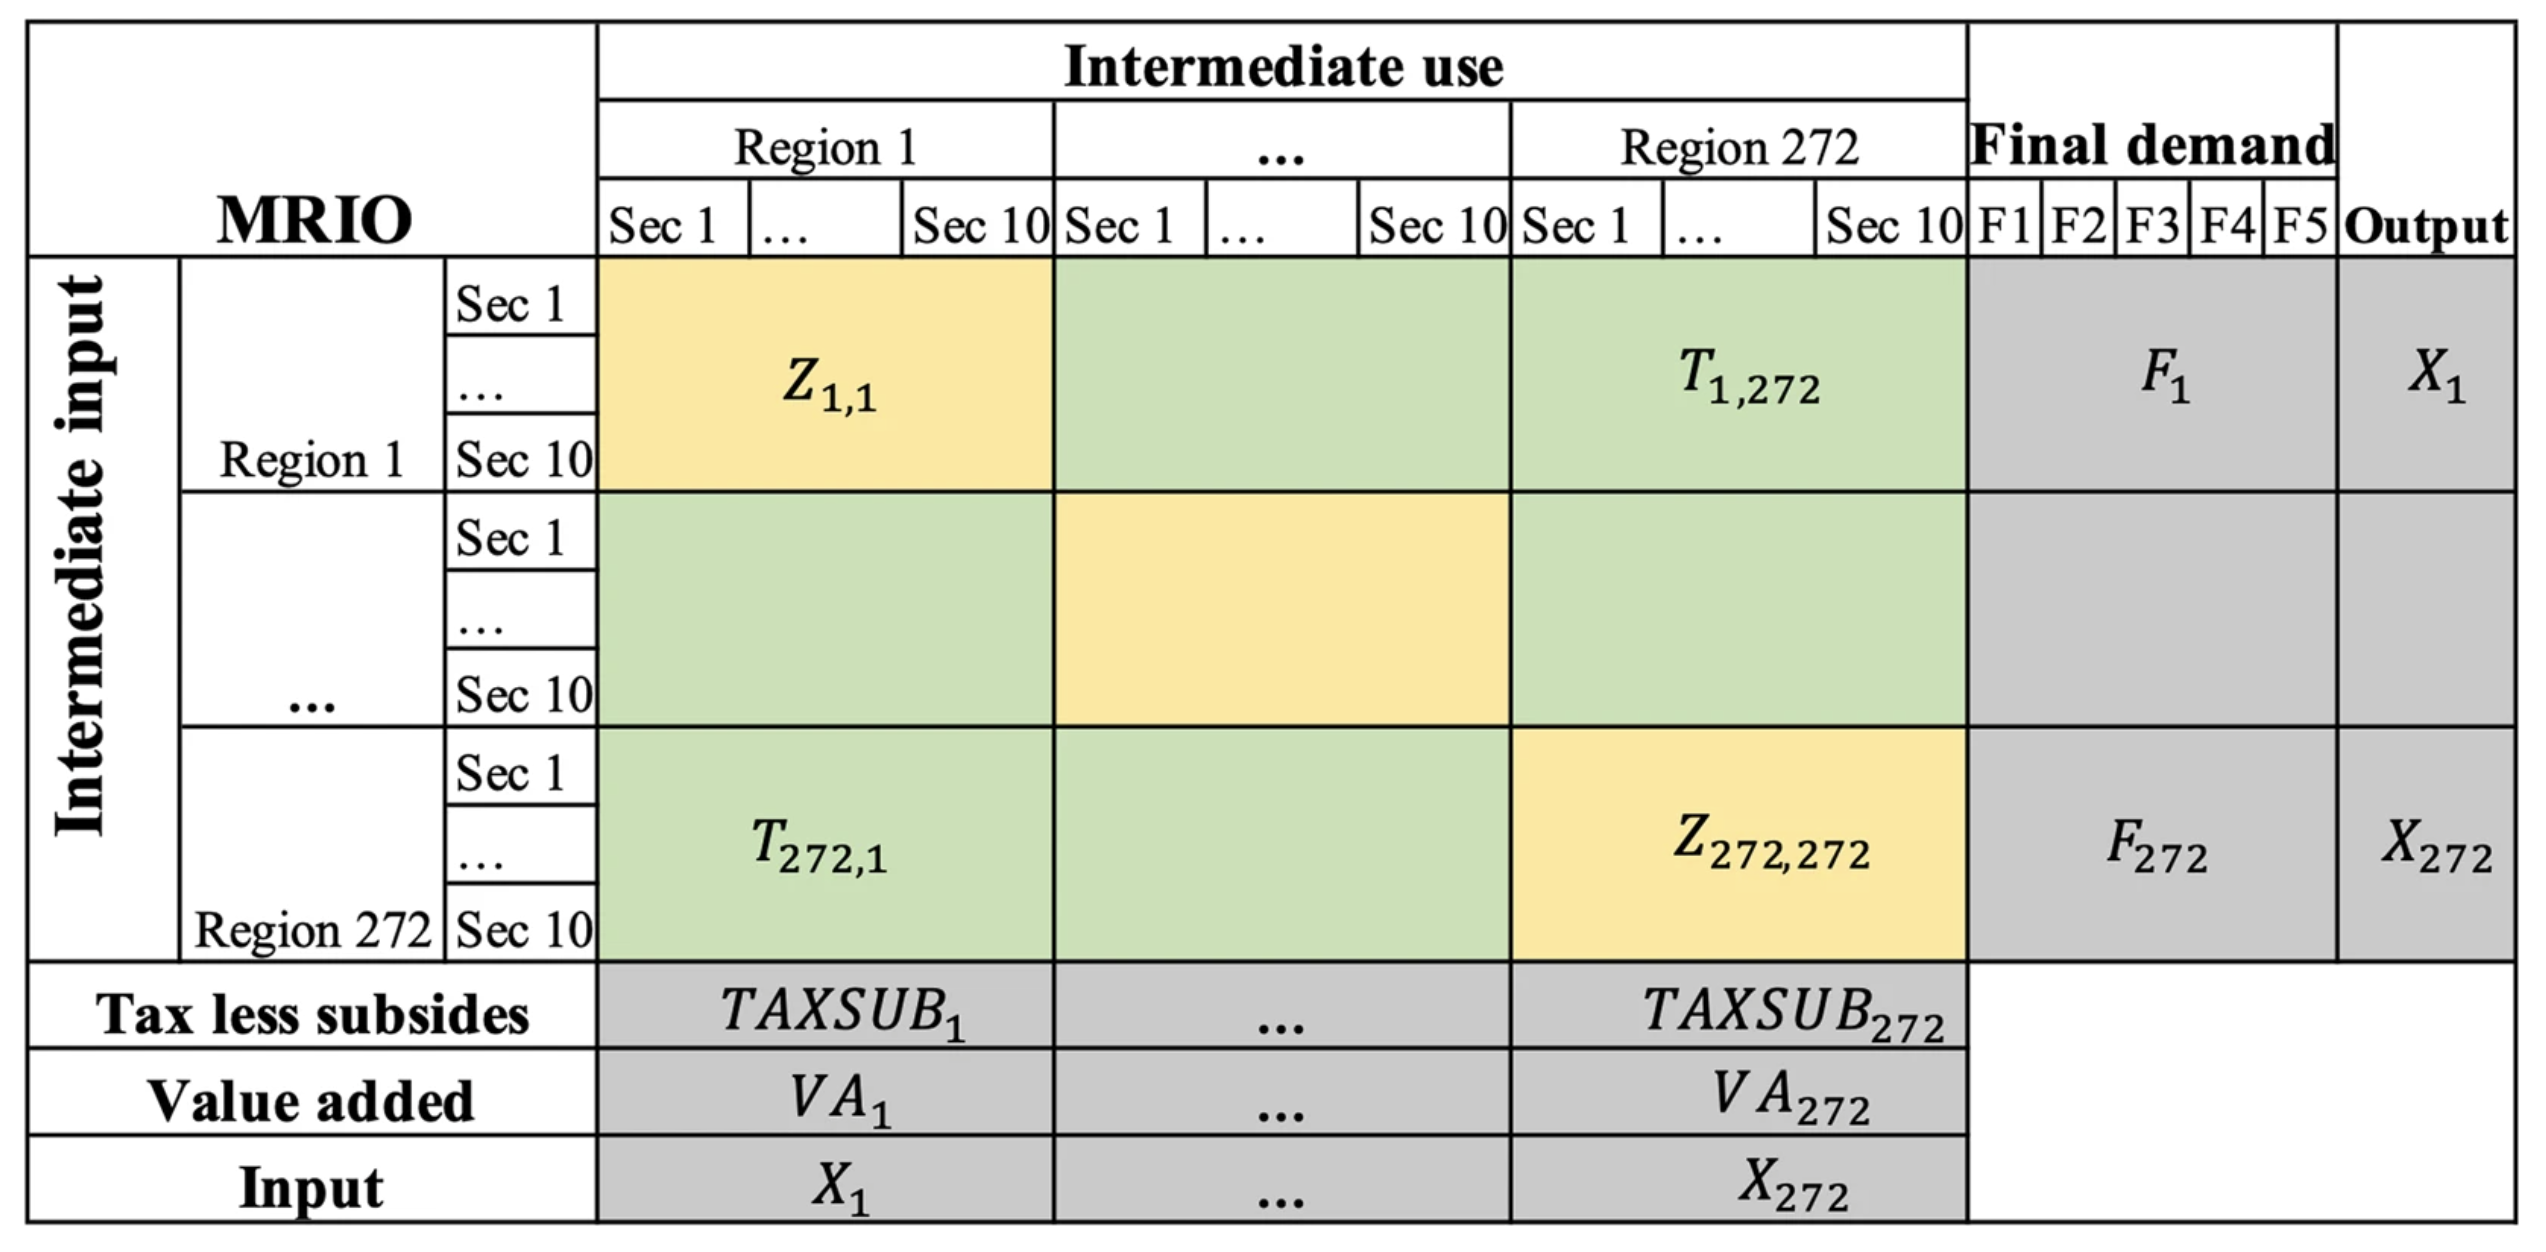
\includegraphics[width=\textwidth]{Figures/MRIO.png}
    \caption[Illustration of a MRIO table]{Illustration of a MRIO table.}
    \label{fig:MRIO}
    \vspace{0.2em}
    {\footnotesize \textit{Source: \cite{ huang_european_2023}}}
\end{figure}

Countries and sectors are indexed by $c = 1, \ldots, n_C$ and $s = 1, \ldots, n_S$, respectively. In EXIOBASE, this corresponds to $n_C = 49$ countries/regions and $n_S = 163$ sectors. Stack all country-sector pairs into a single index $i = 1, \ldots, n$ with $n = n_C n_S$. Let $e_n$ be a $(n \times 1)$ vector of ones and $I_n$ the $(n \times n)$ identity matrix. 

The EXIOBASE database provides the following key matrices and vectors:
\begin{itemize}
    \item The gross output vector $x_t \in \mathbb{R}^{n \times 1}$, where each element represents the total output of a country-sector.

    \item The inter-industry transaction matrix $Z_t \in \mathbb{R}^{n \times n}$, where each element $Z_{ij,t}$ denotes the monetary flow from sector $i$ to sector $j$. Rows correspond to supplying sectors, while columns correspond to using sectors.

    \item The final demand matrix $Y_t \in \mathbb{R}^{n \times n_C n_Y}$, where $n_Y = 7$ denotes the seven categories of final demand: household consumption, consumption by non-profit institutions serving households (NPISH), government consumption, gross fixed capital formation, changes in inventories, changes in valuables, and exports. Each column corresponds to a country-category pair.

    \item The matrix of technical coefficients $A_t \in \mathbb{R}^{n \times n}$, defined as $A_t = Z_t \,\mathrm{diag}(x_t)^{-1}$, where each element $A_{ij,t} = Z_{ij,t} / x_{j,t}$ represents the input from sector $i$ required to produce one unit of output in sector $j$.
\end{itemize}

Let $h^{(c)} \subset \{1, \ldots, n_C n_Y\}$ denote the set of final-demand columns of country $c$ and let $D_H(\mathcal{H})$ be the $(n_C n_Y \times n_C n_Y)$ diagonal selector with ones on indices in $\mathcal{H}$. With these notations, the final demand in country $c$, denoted by $y_t^{(c)}$, is the sum of the $n_Y$ groups for the country, $y_t^{(c)} = Y_t\, D_H\!\left(h^{(c)}\right) e_{n_C n_Y}$. We collect the final demand for all countries and define the total final-demand $(n \times 1)$ vector $y_t = \left(y_t^{(1)}, \ldots, y_t^{(n_C)}\right)e_{n_C}$. These quantities are measured in monetary units.

Total output can be expressed as the sum of intermediate and final demand:
\begin{equation}
x_t = A_t x_t + y_t = (I_n - A_t)^{-1} y_t = \mathcal{L}_t y_t,
\end{equation}
where $\mathcal{L}_t$ denotes the Leontief inverse matrix. 
This equation constitutes the core of the input-output model, linking total production to final demand through direct and indirect independences between economic sectors.

\subsection{Environmental Extensions}
\label{sec:environmental extensions}

We now introduce environmental pressures. For each indicator, EXIOBASE provides 
(i) direct production pressures by industry, measured by the $(1 \times n)$ vector $F_t$, and 
(ii) direct final-use pressures that cannot be attributed to production activities (e.g., fuel combustion in private transport), measured by the $(1 \times n_C n_Y)$ vector $F_{Y,t}$. 

The pressure intensity per unit of output is $S_t = F_t \, \mathrm{diag}(x_t)^{-1}$, and the pressure intensity per unit of final demand is $M_t = S_t\mathcal{L}_t $ (also referred to as the total supply-chain multipliers). The production-related footprint associated with final demand $y_t^{(c)}$ is $M_ty_t^{(c)}$.

The set of industries in country $c$ is denoted by $\mathcal{I}^{(c)} \subset \{1, \ldots, n\}$. Let $D(S)$ denotes the $(n \times n)$ diagonal selector matrix with ones on indices in $S$ and $D_H(\mathcal{H})$ denotes the $(n_C n_Y \times n_C n_Y)$ diagonal selector with ones on indices in $\mathcal{H}$.

While this framework accommodates any EXIOBASE environmental indicator, this thesis primarily focuses on financed emissions. To maintain consistency with the climate-finance literature, the mathematical exposition uses GHG terminology, specifically, emissions ($E$), financed emissions ($FE$) and carbon intensity ($CI$). However, the identical calculations apply to other environmental footprints by substituting the target metric.

In production-based (or territorial) accounting (PBA), the footprint of country $c$ is the sum of direct domestic production pressures and direct domestic final-use pressures:
\begin{equation}
E^{(c)}_{\text{PBA},t} = F_t \, D(\mathcal{I}^{(c)}) \, e_n + F_{Y,t} \, D_H(h^{(c)}) \, e_{n_C n_Y}
\end{equation}

In consumption-based accounting (CBA), the footprint of country $c$ allocates the full supply-chain pressures to domestic final demand, regardless of where pressures occur:
\begin{equation}
E^{(c)}_{\text{CBA},t} = M_t Y_t \, D_H(h^{(c)}) \, e_{n_C n_Y} + F_{Y,t} \, D_H(h^{(c)}) \, e_{n_C n_Y}
\end{equation}

Finally, environmental pressures are attributed to mutually exclusive agent groups. To map industries to real-economy agents, \textit{Private households with employed persons} are assigned to households (HH), \textit{Public administration and defense and compulsory social security} to government (GG), and \textit{Financial intermediation and auxiliary to financial intermediation} to financial institutions (FI). All remaining industries are classified as non-financial corporations (NFC).  

For the mapping from final demand to agents, let $h(k) \subseteq \{1, \ldots, n_C n_Y\}$ denote the set of final-demand columns associated with agent group $k$. Final consumption by households and NPISH is assigned to HH, while government expenditure is assigned to GG. The remaining columns are attributed to NFC; however, final-use pressures for NFC are zero for the indicators considered, as NFC sectors are typically not final users in the economy.

For a given country $c$, environmental footprint attributed to agent group $k$ are defined as
\begin{equation}
E_{k,t}^{(c)} = F_t \, D(\mathcal{I}^{(c)} \cap \mathcal{I}_k)\, e_n 
+ F_{Y,t} \, D_H(h^{(c)} \cap h(k))\, e_{n_C n_Y}
\label{eq:emissions}
\end{equation}

For the rest of the world, I group individual countries into broader regional aggregates, such as North America, Europe, Japan-Pacific, and emerging economies. Environmental footprints are first calculated at the country level. Specifically, for each country $c$ belonging to a given region, I compute $E_{k,t}^{(c)}$ using Equation \ref{eq:emissions}. I then sum these country-level values across all countries in the region to obtain regional totals by real-economy agent group.

Although total foreign claims can be decomposed by region, the effective-exposure matrix obtained from the financial input-output framework identifies foreign issuers only as one aggregate RoW category. Therefore, the regional environmental profiles cannot be directly assigned to separate regional effective exposures. Instead, they are used to construct alternative environmental factors for the aggregate RoW issuer group. This allows the analysis to examine how the estimated environmental footprint of foreign exposures changes under different assumptions about the regional composition of RoW.

\section{Environmental Footprints of Financial Systems}
\label{sec:3.3}

To attribute the environmental pressures generated by real-economy agents to their financiers, I follow the proportional attribution logic used in financed-emissions accounting. Under this approach, environmental pressures are allocated to financial institutions according to their share of financing in the issuer's total financing base, regardless of the specific financial instrument through which the exposure is held. I therefore aggregate all classes of claims, including equity, debt securities, loans, and other financial instruments, into a common attribution base, denoted by $TC_{k,t}$, which represents total claims on real-economy agent group $k$.

For households, however, I follow \textcite{jondeau_environmental_2026} and use total assets rather than total claims, while retaining the notation $TC_{\mathrm{HH},t}$. This adjustment reflects the fact that household environmental pressures arise largely from consumption and asset ownership rather than from debt-financed production activities. Normalizing by total assets therefore provides a more appropriate measure of the economic resources controlled by households and their associated environmental footprint.

The effective, or look-through, exposure of financial-institution category $f$ to real-economy agent group $k$ at time $t$, denoted by $W_{f,k,t}$, is obtained from the matrix $W_{F,t}$ defined in Equation \ref{eq:effective_exposure}. Since funds raised through different financial instruments are treated as part of a common financing base, the attribution factor of institution category $f$ with respect to agent group $k$ is defined as
\begin{equation}
AF_{f,k,t} = \frac{W_{f,k,t}}{TC_{k,t}}.
\end{equation}
The environmental pressure financed by institution category $f$ through its exposure to group $k$ is then given by
\begin{equation}
FE_{f,k,t} = AF_{f,k,t} E_{k,t}
= \frac{W_{f,k,t}}{TC_{k,t}} E_{k,t},
\end{equation}
where $E_{k,t}$ denotes the GHG emissions or other environmental footprint of real-economy agent group $k$. For domestic issuers, $E_{k,t} \equiv E_{k,t}^{(\mathrm{home})}$, as defined in Equation \ref{eq:emissions}. For foreign issuers, $E_{k,t}$ is constructed from the regional environmental profiles described in Section \ref{sec:environmental extensions}. The corresponding attribution base, $TC_{k,t}$, is defined over the same regional coverage, ensuring that environmental footprints and financial claims are measured consistently.

Let $W_{f,t}$ denote the total effective exposure of financial-institution category $f$:
\begin{equation}
W_{f,t} = \sum_{k=1}^{n_R} W_{f,k,t}.
\end{equation}
The total financed environmental footprint of category $f$ is then
\begin{equation}
FE_{f,t}
= \sum_{k=1}^{n_R} \frac{W_{f,k,t}}{TC_{k,t}} E_{k,t}
= W_{f,t} \sum_{k=1}^{n_R}
\underbrace{\frac{W_{f,k,t}}{W_{f,t}}}_{w_{f,k,t}}
\times
\underbrace{\frac{E_{k,t}}{TC_{k,t}}}_{CI_{k,t}}.
\label{eq:financed_emis_fi}
\end{equation}
Equation \ref{eq:financed_emis_fi} shows that the financed environmental footprint of institution category $f$ can be decomposed into two components: the total size of its effective exposure, $W_{f,t}$, and the weighted average environmental intensity of the real-economy agents to which it is exposed. The portfolio weight $w_{f,k,t}$ measures the share of group $k$ in category $f$'s effective exposure, while $CI_{k,t}$ denotes the environmental intensity of group $k$.

At the level of the aggregate financial system, let $W_{k,t}$ denote total effective financing received by real-economy group $k$:
\begin{equation}
W_{k,t} = \sum_{f=1}^{n_F} W_{f,k,t}.
\end{equation}
The total effective exposure of the financial system is
\begin{equation}
W_t = \sum_{k=1}^{n_R} W_{k,t}
= \sum_{f=1}^{n_F} W_{f,t}.
\end{equation}
Aggregating across all financial-institution categories gives
\begin{equation}
FE_t
= \sum_{f=1}^{n_F} \sum_{k=1}^{n_R}
W_{f,t}
\underbrace{\frac{W_{f,k,t}}{W_{f,t}}}_{w_{f,k,t}}
\underbrace{\frac{E_{k,t}}{TC_{k,t}}}_{CI_{k,t}}
= W_t \sum_{k=1}^{n_R} \frac{W_{k,t}}{W_t} CI_{k,t}.
\end{equation}
Thus, the financed environmental footprint of the macro-financial system is the product of total effective financial exposure, $W_t$, and the system-wide weighted average environmental intensity of the real economy.

Although \textcite{jondeau_environmental_2026} discuss the assumptions and robustness of this framework in detail, its key premise is that aggregate financial exposures can be allocated proportionally to the outstanding financing base of each real-economy agent group. The resulting measure should therefore be interpreted as a macro-level attribution of environmental pressures through the structure of financial intermediation. It captures how the financial system as a whole is connected to environmentally intensive activities, rather than the institution-specific portfolio choices that would be observed in micro-level holdings data. 
% Chapter 4
\chapter{Data}
\label{Chapter4} % For referencing the chapter elsewhere, use \ref{Chapter3} 

This chapter describes the datasets used to construct the financial-environmental attribution framework. The analysis combines three main data components. First, from-whom-to-whom financial accounts are used to measure direct and indirect financial exposures across institutional sectors. Second, environmental indicators from EXIOBASE are used to quantify the environmental pressures generated by real-economy agents. Third, balance-sheet data are used to construct the attribution base against which financial exposures are normalized. The final section explains the exchange-rate conversion used to express all monetary variables in a common currency.

\section{From-whom-to-whom matrices}

\textit{FWTW data in the United States. } The Federal Reserve provides FWTW data for each financial instrument, available at \url{https://www.federalreserve.gov/releases/efa/fwtw.htm}
. These data are constructed to align with the issuer, holder, and instrument totals reported in the Financial Accounts. The series is available on a quarterly basis from 1945 to the most recent quarter. 

Table \ref{tab:fwtw_classification} summarizes the sources used to construct the FWTW data for each financial instrument in the United States. As of the fourth quarter of 2022, approximately two-thirds of total asset values are fully specified by \textit{“known relationships”} and \textit{“exclusion restrictions”}, while the remainder relies partially or entirely on proportionality assumptions.

\begin{table}[ht]
\centering
\caption{FWTW data by financial instrument in the US}
\footnotesize
\setlength{\tabcolsep}{4pt}
\renewcommand{\arraystretch}{0.9}

\begin{tabularx}{\textwidth}{>{\raggedright\arraybackslash}p{0.28\textwidth} 
                                  >{\raggedright\arraybackslash}X 
                                  >{\raggedright\arraybackslash}X}
\toprule
\multicolumn{3}{c}{\textbf{Known relationships and exclusion restrictions fully specify FWTW data (\$171.6 trillion as of 2022:Q4)}} \\
\midrule

\multicolumn{3}{l}{
\begin{minipage}{\textwidth}
\vspace{1pt}
\begin{itemize}[leftmargin=*, itemsep=0pt, topsep=0pt]
\item U.S. Official Reserve Assets and SDR Allocations
\item SDR Certificates and Treasury Currency
\item U.S. Deposits in Foreign Countries
\item Net Interbank Transactions
\item Time and Savings Deposits
\item Money Market Funds Shares
\item Treasury Securities
\item Depository Institution Loans N.E.C.
\item Other Loans and Advances
\item Farm Mortgages
\item Consumer Credit
\item Mutual Fund Shares
\item Life Insurance Reserves
\item Pension Entitlements
\item Proprietors' Equity in Noncorporate Business
\item Direct Investment
\item Identified Miscellaneous Financial Claims - I
\item Identified Miscellaneous Financial Claims - II
\end{itemize}
\vspace{1pt}
\end{minipage}
} \\

\midrule

 & \textbf{Single-sector dominated} & \textbf{Multi-sector balanced} \\
\midrule

\textbf{Known relationships, restrictions, and proportionality assumptions} 
& (\$19.4T as of 2022:Q4)
\begin{itemize}[leftmargin=*, itemsep=0pt, topsep=0pt]
\item Municipal Securities
\item Home Mortgages
\item Multifamily Residential Mortgages
\end{itemize}
& (\$33T as of 2022:Q4)
\begin{itemize}[leftmargin=*, itemsep=0pt, topsep=0pt]
\item Checkable Deposits and Currency
\item Federal Funds and Repos
\item Open Market Paper
\item Corporate and Foreign Bonds
\item Taxes Payable
\end{itemize} \\

\midrule

\textbf{Proportionality assumptions only} 
& (\$15.3T as of 2022:Q4)
\begin{itemize}[leftmargin=*, itemsep=0pt, topsep=0pt]
\item Agency- and GSE-Backed Securities
\item Commercial Mortgages
\end{itemize}
& (\$19.4T as of 2022:Q4)
\begin{itemize}[leftmargin=*, itemsep=0pt, topsep=0pt]
\item Trade Credit
\item Unidentified Miscellaneous Financial Claims
\end{itemize} \\

\bottomrule
\end{tabularx}

\vspace{4pt}
\begin{minipage}{\textwidth}
\footnotesize
\textit{Source: The Federal Reserve}
\end{minipage}

\label{tab:fwtw_classification}
\end{table}

Raw FWTW data in the United States are provided with information on instrument names (and codes), holder names (and codes), issuer names (and codes), as well as the corresponding date and level. This thesis uses fourth-quarter observations spanning from 2000 to 2024. 

Following the classification outlined in Section \ref{Section 3.1.2}, holders and issuers are aggregated into four real-economy sectors and five financial institution categories. To account for discrepancies, an additional row and column are introduced, resulting in a $10 \times 10$ matrix for each financial instrument. These instruments are then consolidated into ten major asset classes, and the matrix construction procedure is repeated annually over the sample period.

% ---------------
\textit{FWTW data in the euro area.} Compared to the United States, the processing and construction of FWTW matrices in the Euro area is more complex. Financial accounts and FWTW-related data for EU member states and the Euro area are published by the ECB within a comprehensive dataset known as the \textit{Quarterly Sector Accounts}, which contains 369{,}626 time series. To navigate this dataset, it is necessary to consult the accompanying catalogue, which provides a complete list of series and their associated metadata and is available at \href{https://data.ecb.europa.eu/data/data-categories/2045085/data-information?layerType=KL&showDatasetModal=false}{this link}.

For each financial instrument, the catalogue is filtered to retain only quarterly euro area series (\texttt{ref\_area = I9}), reported on an end-of-period basis (\texttt{time\_per\_collect = E}), and at the total level of breakdown (\texttt{cust\_breakdown = \_T}). For loans and deposits, which are further disaggregated by maturity in the ECB database, only total-maturity series (\texttt{maturity = T}) are retained to avoid duplication. The dataset is further restricted to series for which both the reporting sector (\texttt{ref\_sector}) and the counterpart sector (\texttt{counterpart\_sector}) belong to the set of institutional sectors defined in the previous classification.

Once the relevant series have been identified, the associated series codes are used to query the ECB Data API and retrieve the corresponding observations, which are then combined by instrument and exported as separate CSV files. Each series includes a field indicating whether the position is recorded as an asset or a liability from the perspective of the reporting sector; this information is used to identify the holder and issuer of the corresponding instrument.

The ECB provides complete FWTW matrices for a subset of instruments, including deposits, debt securities, loans, listed shares, money market fund shares, and
mutual fund shares. However, the time coverage differs across instruments: for some instruments, complete FWTW information is available only from 2013 onward.
For the remaining instruments and periods, the ECB reports only aggregate row and column totals through the financial accounts. To address this limitation, I
define ``restriction exclusions'' and identify available ``known relationships.'' I then apply the IPFP algorithm to estimate and populate the missing interior
entries of the matrix. Table~\ref{tab:fwtw_eu} summarizes which instruments are directly sourced from the ECB and which are constructed using this methodology.
The structural restrictions imposed for each financial instrument are presented in Appendix~\ref{Appendix A: Structural Restrictions}.

As discussed in Section~\ref{sec:FWTW_introduction}, total issuance may not equal total holdings for some financial instruments. In such cases, the algorithm is set to match the row sums, i.e., the total holdings of each sector for the corresponding instrument. The main reason for prioritizing row balancing over column balancing is to ensure comparability with US FWTW data, where a similar approach is adopted, resulting in a zero discrepancy (DIS) column. To reconcile remaining inconsistencies, discrepancy (DIS) rows and columns are introduced so that the matrices are consistent with aggregate totals reported in the financial accounts.
\begin{table}[ht!]
\centering
\caption{FWTW data by financial instrument in the Euro area}
\label{tab:fwtw_eu}
\small
% Note: \textwidth makes it fit exactly to the page margins
\begin{tabularx}{\textwidth}{@{} 
    >{\raggedright\arraybackslash}p{3cm} 
    >{\raggedright\arraybackslash}X 
    l 
    >{\centering\arraybackslash}p{2.5cm} 
    >{\centering\arraybackslash}p{2.5cm} 
    @{}}
\toprule
\textbf{Group} & \textbf{Instruments} & \textbf{Code} & \textbf{FWTW by ECB} & \textbf{FWTW by author} \\
\midrule
% ---------------------------------------------------------
\textbf{Monetary Gold and SDRs} & Monetary gold and SDRs & F1 & & \checkmark \\
\midrule
% ---------------------------------------------------------
\textbf{Currency and Deposits} & Currency & F2M &  & \checkmark \\
& Deposits & F21 & \checkmark &  \\
\midrule
% ---------------------------------------------------------
\textbf{Debt securities} & Debt securities (*) & F3 & \checkmark  & \checkmark \\
 & & & (2013-2024) & (2000-2012) \\
\midrule
% ---------------------------------------------------------
\textbf{Loans} & Loans & F4 & \checkmark & \\
\midrule
% ---------------------------------------------------------
\textbf{Equity} & Listed shares & F511 & \checkmark & \checkmark\\
 & & & (2013-2024) & (2000-2012) \\
& Unlisted shares & F512 & & \checkmark \\
& Other equity & F519 & & \checkmark \\
\midrule
% ---------------------------------------------------------
\textbf{Money Market Funds Shares} & Money market fund shares (**) & F521 & \checkmark & \checkmark \\
 & & & (2013-2024) & (2000-2012) \\
\midrule
% ---------------------------------------------------------
\textbf{Mutual Fund Shares} & Non-MMF investment fund shares (**) & F522 & \checkmark & \checkmark \\
 & & & (2013-2024) & (2000-2012) \\
\midrule
% ---------------------------------------------------------
\textbf{Insurance} & Life insurance & F62 & & \checkmark \\
& Non-life insurance technical reserves and provision for calls under standardised guarantees & F6O & & \checkmark \\
\midrule
% ---------------------------------------------------------
\textbf{Pension} & Pension schemes & F6M & & \checkmark \\
\midrule
% ---------------------------------------------------------
\textbf{Other} & Financial derivatives & F7 & & \checkmark \\
& Other accounts receivable & F8 & & \checkmark \\
\bottomrule
\end{tabularx} 

\vspace{4pt}
\begin{minipage}{\textwidth}
\footnotesize
\textit{Source: Author's compilation.}\\

(*) The ECB provides the full matrix for debt securities from 2013 onward. Before 2013, only row and column totals are available from the financial accounts. The ECB also reports holdings of debt securities issued by and held within non-financial corporations, which is used as a known relationship in the estimation.\\

(**) All sectors hold money market fund (MMF) and mutual fund (non-MMF) shares, but issuance is limited to RoW and MFI (for MMF shares) and NM\_MFIF (for non-MMF shares). From 2013 onwards, ECB reports, for each sector, holdings of shares issued by MFI (and NM\_MFIF), but provides only total issuance for RoW. As there are only two issuers, the RoW column is derived residually as total holdings minus the MFI (or NM\_MFIF) column. 
\end{minipage}
\end{table}

\textit{Discrepancies.} While it is important to verify that each component sums to the aggregate macroeconomic totals, discrepancies do not have economic substance as either real-economy agents or financial institutions. Accordingly, after aggregating the FWTW matrices across all asset classes (see Section~\ref{sec:effective_financing}), I exclude the discrepancy row and column from subsequent steps when computing effective exposures. Although discrepancies can account for a substantial share of issuance or holdings for certain financial instruments (e.g., monetary gold and SDRs), their aggregate importance remains limited. In particular, total discrepancies remains below 3 percent in the United States and below 1 percent in the Euro area of total issuance across all financial assets for any years in the 2000-2022 period. Detailed figures are presented in Appendix \ref{Appendix B:Total_dis}.

\section{Environmental indicators}

To quantify the environmental pressures generated by real-economy agents, I utilize EXIOBASE v3, an \textit{environmentally extended multi-regional input-output} (EE-MRIO) database that captures the global web of economic relationships and their corresponding environmental impacts \citep{stadler_exiobase_2018}. Input-output modelling is a well-established framework that traces monetary flows between industries and end-users to represent global production and consumption structures. By integrating environmental satellite accounts, this framework enables the quantification of pressures such as greenhouse gas emissions, land and water use, and material extraction, tracing them along international supply chains \citep{hauschild_life_2018, leclerc_building_2020}. EXIOBASE v3 is one of the most comprehensive EE-MRIO databases available, covering 44 individual countries and five RoW regions, disaggregated into 163 industries, with an annual time series spanning 1995 to 2022.

Although the attribution framework detailed in Chapter \ref{Chapter3} can accommodate any environmental indicators available in EXIOBASE v3, this thesis focuses on four key dimensions of environmental impact. For each dimension, I extract direct production pressures ($F_t$) and direct final-use pressures ($F_{Y,t}$) from the respective EXIOBASE impact accounts:

\begin{itemize}
    \item \textbf{Climate Change:} Greenhouse gas emissions, captured via the \texttt{GHG emissions GWP100 IPCC2010} account. This aggregates carbon dioxide (CO$_2$), methane (CH$_4$), and nitrous oxide (N$_2$O) into kilograms of carbon dioxide equivalents (kg CO$_2$e) using the 100-year Global Warming Potentials established by the IPCC.
    \item \textbf{Land Use:} Total land occupation, measured in square kilometers (km$^2$).
    \item \textbf{Water Consumption:} Blue water consumption, measured in millions of cubic meters (Mm$^3$).
    \item \textbf{Resource Extraction:} Domestic extraction of four primary material categories, including fossil fuels, iron ore, non-ferrous metal ores, and non-metallic minerals, measured in kilotonnes (kt).
\end{itemize}

Choosing EXIOBASE v3 over other global EE-MRIO databases, such as Eora, the OECD Inter-Country Input-Output Tables (ICIO), and the World Input-Output Database (WIOD), involves several methodological trade-offs.

\textit{Advantages.} EXIOBASE v3 is particularly suitable for this thesis because of the breadth, comparability, and recent coverage of its environmental satellite accounts. While WIOD \citep{timmer_illustrated_2015} and the OECD ICIO \citep{oecd_inter-country_2026} provide reliable economic input-output data, they were primarily designed for macroeconomic and trade analysis. Their environmental extensions are therefore more limited, focusing mainly on energy use, CO$_2$, or GHG emissions. In addition, the most comprehensive WIOD environmental satellite accounts end in 2016, which limits their usefulness for analysing recent macro-financial exposures.

By contrast, EXIOBASE v3 provides annual data up to 2022 and covers a wide range of environmental pressures, including greenhouse gas emissions, land use, water use, energy use, and material extraction \citep{stadler_exiobase_2018}. This makes it possible to conduct a multi-dimensional assessment of the environmental footprint of financial systems, rather than focusing only on climate-related indicators.

EXIOBASE also offers an advantage in terms of sectoral and environmental harmonisation. Eora, for example, provides broader geographic coverage and preserve national input-output tables in their original classifications, but this heterogeneous structure can make cross-country comparisons more difficult and may require additional harmonisation \citep{lenzen_building_2013, casella_unctad_2019}. More generally, differences in classification, aggregation, and database construction choices can lead to non-negligible deviations in footprint estimates across MRIO databases \citep{giljum_impacts_2019}. In this context, the relatively detailed and harmonised structure of EXIOBASE makes it well suited for comparing environmental pressures across the United States and the Euro area.

\textit{Limitations.} Despite its advantages, EXIOBASE presents several limitations relevant to this thesis. First, data for the most recent years are not derived entirely from primary source tables. Although recent EXIOBASE releases extend the time series to 2022, the final years rely on macroeconomic indicators, trade data, and available environmental proxies rather than complete supply-use tables for all countries and sectors \citep{stadler_exiobase_2018}. Consequently, short-term fluctuations in the latest years of the sample, particularly between 2020 and 2022, should be interpreted with caution.

Second, EXIOBASE trades geographic resolution for sectoral and environmental detail. The database explicitly covers 44 countries alongside five aggregate RoW regions. While this structure is well-suited for analysing major economies like the United States and the Euro area, it restricts the ability to capture nuances within developing and emerging economies. Grouping countries with distinct production structures, resource endowments, and environmental intensities into broad RoW regions can obscure substantial local heterogeneity. This is particularly problematic for spatially specific environmental pressures, such as land use, water stress, and biodiversity impacts. Indeed, studies increasing the geographic resolution of EXIOBASE demonstrate that disaggregating RoW regions can materially alter footprint estimates \citep{bjelle_adding_2020, cabernard_highly_2021}.

While these constraints do not undermine EXIOBASE's suitability for this analysis, they must inform how the results are interpreted. Therefore, the estimates presented here should be viewed as harmonised, macro-level footprints of financial systems rather than precise, country-level measures of individual foreign exposures.
\section{Attribution Base}

The attribution base, denoted by $TC_{k,t}$, represents the total claims on real-economy agents $k \in \{\text{NFC}, \text{GG}, \text{RoW}\}$ and the total assets for household sector, where $k = \text{HH}$ (see Section \ref{sec:3.3} for a detailed explanation). For domestic sectors, total claims can be extracted from financial accounts, corresponding to the column sums of the aggregated FWTW matrices. To determine total assets for HH, the net worth of household sector, that is available in financial accounts, is added to total claims on HH. 

For the RoW, the OECD Financial Accounts and Balance Sheets database\footnote{Source: \url{https://www.oecd.org/en/data/datasets/financial-accounts-and-balance-sheets.html}} provides sector-level balance sheets for OECD and several non-OECD countries, serving as a reliable source for indicative figures of the RoW's total claims. Specifically, the total claims of the RoW sector aggregate the liabilities of foreign non-financial corporations, general governments, and financial institutions. The foreign household sector is explicitly excluded from this aggregation, under the assumption that domestic financial institutions do not typically extend direct loans or credit to foreign households. Although this dataset covers 42 countries, only those also covered by the EXIOBASE v3 database are used to construct the RoW attribution base to ensure a consistent and fair attribution factor. By definition, the home country or region (e.g., the US or the Eurozone) is excluded from the calculation of the RoW's total claims. Finally, Appendix \ref{Appendix C:Countries} provides a comprehensive list of countries covered by the OECD and EXIOBASE v3 databases, their regional grouping, the member states of the Eurozone, and the specific countries that constitute the "Rest of World" for the US and Euro area. 

A major advantage of the OECD database is that it is harmonized under the 2008 SNA framework. However, it excludes China, a critical omission given that China holds the second-highest national debt (\cite{world_population_review_countries_2026}) and is the leading global GHG emitter (\cite{european_commission_joint_research_centre_ghg_2025}). To address this gap and align with EXIOBASE v3, which explicitly captures China’s environmental pressures, I incorporate China's financial accounts into the analysis. Specifically, for the broadest RoW scenario, I integrate China's data into the attribution base of the RoW sector for both the US and the Euro area.

In 2020, the People’s Bank of China (PBC) published data on the levels of financial assets and liabilities, i.e., sectoral balance sheets, on its official website for the first time.\footnote{Available at \url{https://www.pbc.gov.cn/en/3688247/3688975/index.html}.} The published series were backfilled to 2017. To bridge the data gap in analyses of China’s macroeconomic operations, academic studies have also used China’s sovereign balance sheets compiled by \textcite{li_yang_chinas_2020} at the Centre for National Balance Sheet, which cover the period 2000-2019.
I compare the overlapping years, 2017-2019, between the two sources (see Table \ref{tab:china_comparison}). The comparison shows that the combined liabilities of NFCs, general government, and financial institutions reported by \textcite{li_yang_chinas_2020} are approximately 35-36\% higher than the corresponding official figures published by the People’s Bank of China in each of the three overlapping years. To ensure consistency with the official PBC series, I therefore adjust the total liabilities of NFCs, general government, and financial institutions from the Centre for National Balance Sheet for the period 2000-2016 downward by the average difference 36.26\%, under the assumption that the structural reporting variance between the academic and official accounts remained relatively stable over the historical period.

\begin{table}[H]
\centering
\renewcommand{\arraystretch}{1.3} 
\caption{China's financial accounts by different sources in \\overlapping years}
\label{tab:china_comparison}

\makebox[\textwidth][r]{\footnotesize Unit: 100 Million Yuan}\vspace{2pt}

\resizebox{\textwidth}{!}{
\begin{tabular}{l r r r r r r r r r}
\toprule
 & \multicolumn{4}{c}{\textbf{The People's Bank of China}} & \multicolumn{4}{c}{\textbf{The Centre for National Balance Sheet}} & \\
\cmidrule(lr){2-5} \cmidrule(lr){6-9}
 & \multicolumn{1}{c}{NFC} & \multicolumn{1}{c}{GG} & \multicolumn{1}{c}{FI} & \multicolumn{1}{c}{\cellcolor{blue!15}NFC+GG+FI} & \multicolumn{1}{c}{NFC} & \multicolumn{1}{c}{GG} & \multicolumn{1}{c}{FI} & \multicolumn{1}{c}{\cellcolor{blue!15}NFC+GG+FI} & \multicolumn{1}{c}{\% Change} \\
 & \multicolumn{1}{c}{\textit{(1)}} & \multicolumn{1}{c}{\textit{(2)}} & \multicolumn{1}{c}{\textit{(3)}} & \multicolumn{1}{c}{\cellcolor{blue!15}\textit{(4) = (1)+(2)+(3)}} & \multicolumn{1}{c}{\textit{(5)}} & \multicolumn{1}{c}{\textit{(6)}} & \multicolumn{1}{c}{\textit{(7)}} & \multicolumn{1}{c}{\cellcolor{blue!15}\textit{(8) = (5)+(6)+(7)}} & \multicolumn{1}{c}{\textit{(9)=(8)/(4) - 1}} \\
\midrule
2017 & 1,875,034 & 416,104 & 3,733,134 & \cellcolor{blue!15}6,024,272 & 3,827,714 & 299,051 & 4,027,658 & \cellcolor{blue!15}8,154,423 & 35.36\% \\
2018 & 1,833,366 & 494,401 & 3,843,805 & \cellcolor{blue!15}6,171,572 & 3,947,967 & 332,666 & 4,160,287 & \cellcolor{blue!15}8,440,920 & 36.77\% \\
2019 & 2,073,460 & 561,773 & 4,081,652 & \cellcolor{blue!15}6,716,885 & 4,392,160 & 379,577 & 4,406,288 & \cellcolor{blue!15}9,178,025 & 36.64\% \\
\midrule
 & & & & & & & & \cellcolor{blue!15}\textbf{\textit{Average}} & 36.26\% \\
\bottomrule
\end{tabular}
}
\vspace{1pt}\\
\begin{minipage}{\textwidth}
\footnotesize\textit{Source: The People's Bank of China and The Centre for National Balance Sheet}
\end{minipage}
\end{table}

\section{Foreign Exchange}

To ensure comparability across datasets, all monetary variables are converted into a common reporting currency, the US dollar. Specifically, end-of-year spot exchange rates are employed to maintain temporal consistency. The Chinese Yuan Renminbi is converted into U.S. dollars using the Chinese Yuan Renminbi to U.S. Dollar spot exchange rate (DEXCHUS)\footnote{Source: \url{https://fred.stlouisfed.org/series/DEXCHUS}}, while values originally denominated in euros are converted using the U.S. Dollar to Euro spot exchange rate (DEXUSEU)\footnote{Source: \url{https://fred.stlouisfed.org/series/DEXUSEU}}. Both series are obtained from the \textit{Federal Reserve Economic Data (FRED)} database maintained by the Federal Reserve.
% Chapter 5
\chapter{Empirical Results} % Main chapter title
\label{Chapter5} 

This chapter presents the empirical results of the financial-environmental attribution framework, analyzing and contrasting the environmental pressures financed by the financial systems of the United States and the Euro area. By mapping macro-financial asset allocations to physical environmental flows, the analysis reveals how distinct institutional structures and geographic investment strategies drive global environmental profiles. 

The chapter is structured as follows: Section \ref{sec:6.1} explores the structural evolution of financial exposures across institutional categories and real-economy agents, establishing the macroeconomic foundations of both systems. Section \ref{sec:6.2} evaluates financed emissions, decomposing portfolio footprints through regional scenarios and comparing them against traditional production- and consumption-based accounting benchmarks. Finally, Section \ref{sec:6.3} expands the attribution framework beyond carbon metrics to evaluate multi-dimensional ecosystem pressures, focusing on land use, blue-water consumption, and upstream resource extraction.

\section{Financial Exposures Across Institutions and Economic Agents}
\label{sec:6.1}

Figure \ref{fig:total_exp_fi} illustrates the evolution of total financial institution exposure in the US and the EZ, revealing substantial differences in the financial structures of the two regions. The Euro area features a "bank-based" system, where monetary financial institutions are the predominant source of economic financing. In contrast, the proportion of finance channeled through non-bank institutions is significantly higher in the US. This aligns with the well-documented characterization of the US as a "market-based" system, where funds are raised primarily through securities markets \citep{de_fiore_bank_2005, bats_bank-based_2020}. \textcite{de_fiore_bank_2005} attributes these structural differences to the lower availability of public information regarding firms' creditworthiness in the Euro area, coupled with the higher efficiency of its banks in acquiring this information. Recognizing these distinct financial frameworks is crucial for analyzing how exposure evolves over time. For example, research indicates that bank-oriented systems are more susceptible to financial crises and systemic risks than market-based systems, suffering higher rates of bank defaults during economic downturns \citep{gambacorta_financial_2014, bats_bank-based_2020}. This inherent vulnerability helps explain the severe post-2008 contraction of banking assets in the Euro area, which did not recover to pre-crisis levels until after 2020. In contrast, the US financial system experienced only a temporary slowdown and avoided comparable systemic deterioration.

Another noticeable difference between the US and the EZ is the size of pension fund assets under management. While pension fund exposure in the Euro Area has remained relatively limited over time, in the United States pension funds have consistently been as a large and important channel of financial intermediation. This gap largely reflects the prevalence of two distinct pension systems across the regions: pay-as-you-go (PAYG) and capital-funded schemes. PAYG systems, where current contributions are used to finance current retirement benefits, remain dominant in the Euro Area, particularly in populated countries such as Germany, Italy, and France \citep{van_der_zwan_financialisation_2017}. In contrast, the US system relies more heavily on capital-funded pensions, in which workers’ contributions are invested in financial markets and retirement benefits are financed through accumulated returns. Combined with a relatively flexible regulatory environment that permits higher exposure to equities and alternative assets, this structure has enabled substantial asset accumulation over time. Moreover, US pension fund growth has been significantly supported by strong equity market performance, particularly the expansion of the technology sector over the past two decades \citep{andonov_pension_2017}.

Lastly, the activity level of Other Financial Institutions, a common proxy for the shadow banking sector, is not only substantial but has also experienced considerable growth in both regions. As defined in Section \ref{sec:fi_def}, this category includes issuers of asset-backed securities (ABS) and special purpose vehicles (SPVs) that facilitate the securitization process. Prior to 2008, OFI exposure even exceeded that of the traditional banking sector in the US, illustrating the buildup of unregulated securitization that is widely recognized as a primary catalyst for the 2008-2009 Global Financial Crisis \citep{brunnermeier_deciphering_2009}. In the Euro area, a post-crisis substitution effect emerged: the contraction of the traditional banking sector was offset by the expanding activities of the shadow banking sector. However, this growth trajectory has largely stagnated since 2017. This plateau can be primarily attributed to the gradual recovery of traditional bank lending capacities and the introduction of stricter regulatory frameworks aimed at reducing shadow banking risks \citep{european_systemic_risk_board_eu_2018}.

\begin{figure}[h]
    \centering
    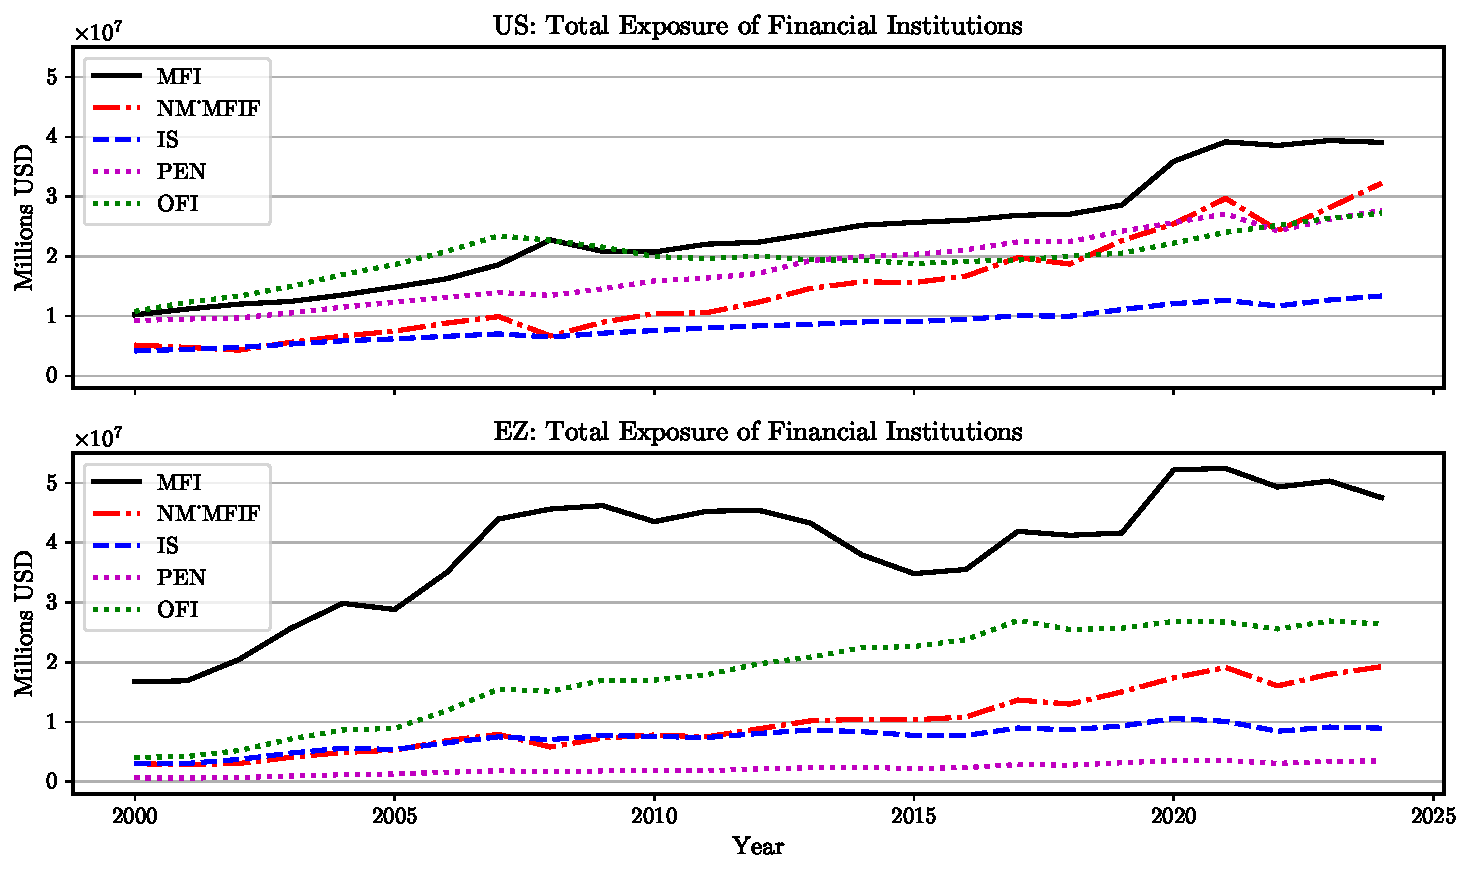
\includegraphics[width=1\textwidth]{Figures/FI_TotalExposure_US_vs_EZ_Institutions.pdf}  
    \caption{Total exposure of Financial Institutions: US and EZ}
    \label{fig:total_exp_fi}
\end{figure}

Figure \ref{fig:total_exp_agent} illustrates which real-economy sectors are financed by regional financial systems. Because these real-economy agents directly impact the environment, identifying them clarifies the core drivers of environmental pressures linked to financing activities. In the US, domestic corporations have consistently remained the largest debt holders. Prior to 2008, both households and the corporate sector received equal funding from financial institutions and experienced a decade of rapid expansion. Following the financial crisis, however, stricter regulations largely halted funding to the household sector. Similarly, the corporate sector was the primary recipient of funding in the Euro area until 2012, marking the peak of the Eurozone debt crisis. Since then, Eurozone financial corporations have increasingly redirected their funding flows outward to foreign markets.

We can also see a divergence in how government debt is financed across the two regions. In the US, the financial system is a massive internal funding engine for the government. This reflects the role of US Treasuries as a foundational safe asset; under post-2008 frameworks like Basel III's Liquidity Coverage Ratio (LCR), domestic institutions face strict requirements to hold High-Quality Liquid Assets (HQLA) to ensure liquidity, driving massive captive demand for government debt \citep{he_agency_2022}. Conversely, Eurozone internal government financing has remained notably stagnant since the 2012 debt crisis. Academic literature on the "bank-sovereign nexus", often called the 'doom loop', helps explain this stagnation. During the crisis, as government debt lost value, the domestic banks holding that debt faced insolvency, which in turn forced governments deeper into debt to rescue them \citep{alogoskoufis_regulating_2018, hristov_macroprudential_2021}. Post-crisis efforts have sought to discourage European financial institutions from over-concentrating in domestic sovereign debt to mitigate this systemic risk \citep{soenen_drivers_2020}. Furthermore, the European Central Bank's prolonged era of negative interest rate policies depressed domestic yields, driving Eurozone banks to search for yield and increasingly redirect their lending flows outward across borders \citep{andreeva_negative_2023}.

\begin{figure}[h]
    \centering
    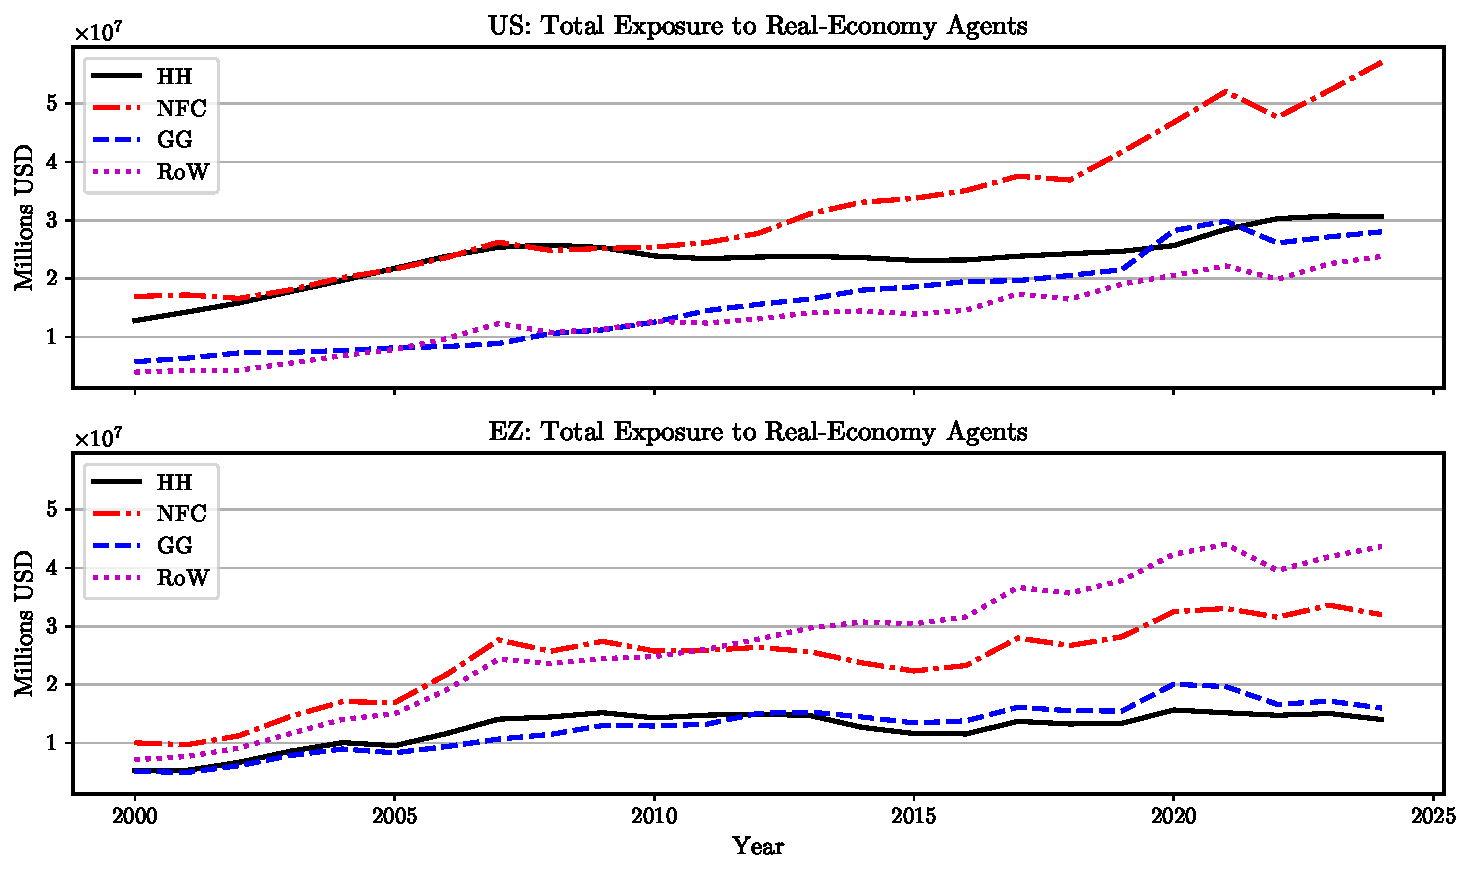
\includegraphics[width=1\textwidth]{Figures/FI_TotalExposure_US_vs_EZ_Agents.pdf}
    \caption{Total exposure to Real-Economy Agents: US and EZ}
    \label{fig:total_exp_agent}
\end{figure}

Overall, the total exposure of the financial system has been larger in the US compared to the Eurozone for most of the observed period (see Figure \ref{fig:total_exp}). While both regions followed similar growth trajectories early on, a significant divergence emerged post-2020, with US exposure accelerating faster. At the end of 2024, the exposure of financial system in the US was 139.6 trillion USD versus 105.7 trillion USD in the EZ. Regarding portfolio composition, the US financial system has consistently maintained a strong domestic focus, allocating over 80\% of its exposure to domestic sectors. In contrast, the Eurozone exhibits a much higher propensity to finance foreign agents, with the RoW sector expanding to account for roughly 40\% of its total exposure by the end of the period.  

\begin{figure}[h]
    \centering
    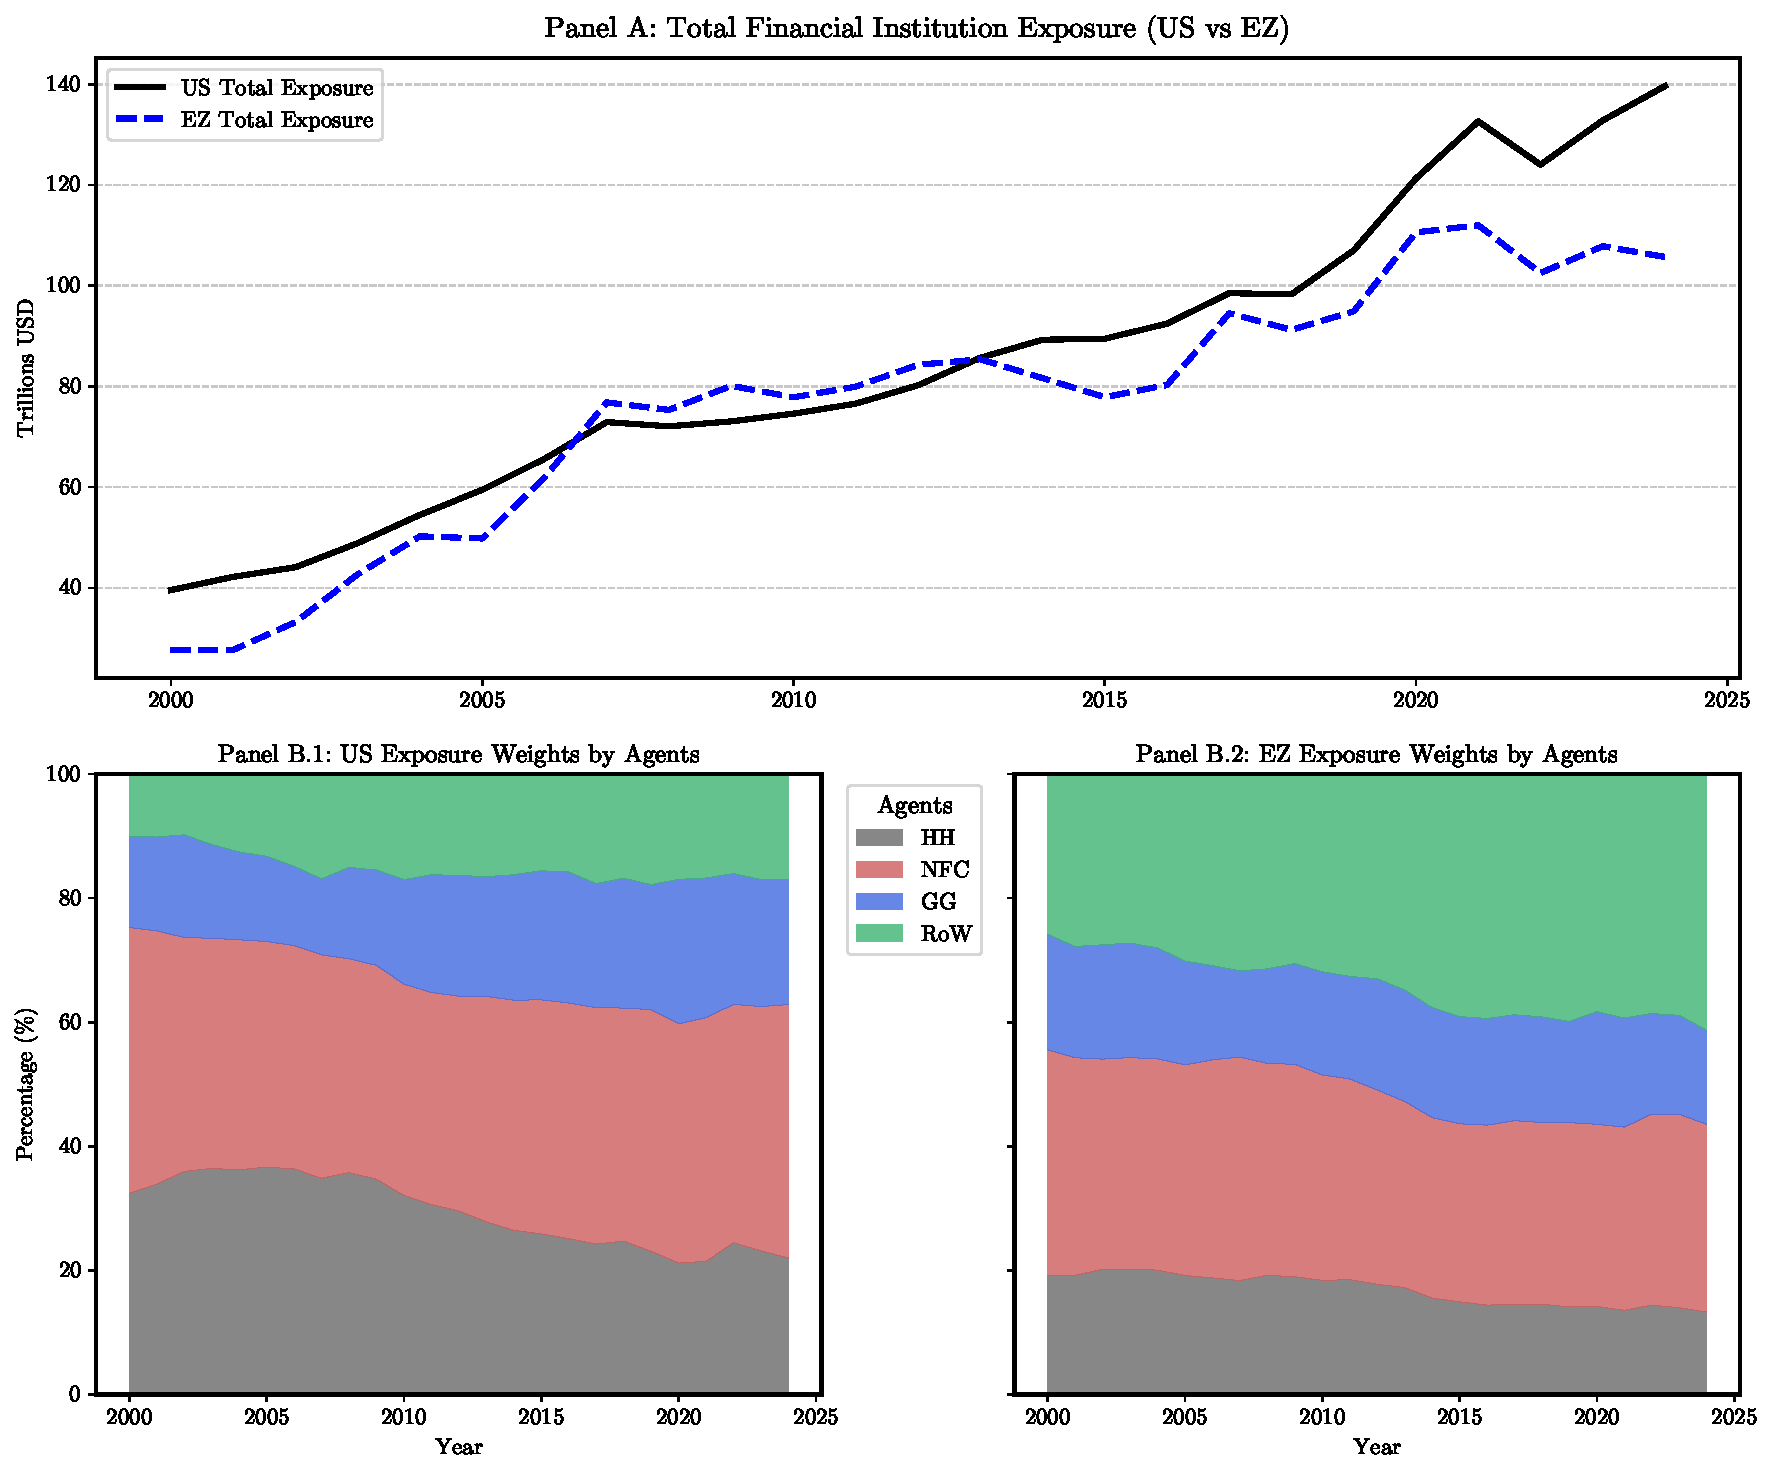
\includegraphics[width=1\textwidth]{Figures/US_vs_EU_Exposure_and_Weights.pdf}
    \caption{Total exposure of the whole financial system and exposure weights by agents}
    \label{fig:total_exp}
\end{figure}

\section{Financed Emissions}
\label{sec:6.2}

\subsection{Carbon Intensity}

The remaining component in calculating total financed emissions in Equation \ref{eq:financed_emis_fi} is the carbon intensity of real-economy agents, defined as the ratio of GHG emissions to their total financial claims ($CI_{k,t}=\frac{E_{k,t}}{TC_{k,t}}$). Because carbon intensity is a ratio, fluctuations can be driven by either numerator effects (changes in absolute emissions) or denominator effects (expansions or contractions in total financial claims). While the following analysis focuses on the resulting intensity trajectories, a full temporal decomposition of the absolute emissions and total claims driving these trends is provided in Appendix \ref{Appendix D:Decompostion}. 


Figure \ref{fig:intensity_dom} reports the carbon intensity of domestic agent groups in the US and the EZ. Over the past two decades, this intensity has steadily declined for all agents across both regions. The government sector consistently exhibits the lowest values, as its associated emissions are primarily confined to public administration activities. By 2022, government carbon intensity stood at approximately 3 $\text{tCO}_2\text{e}$ per million USD for the US, and 3.7 $\text{tCO}_2\text{e}$ per million USD for the Euro area.

The household sector also demonstrates a relatively low carbon intensity that is highly comparable between the two regions. In the US, household intensity dropped significantly from 45.4 $\text{tCO}_2\text{e}$ per million USD in 2000 to 10.7 $\text{tCO}_2\text{e}$ per million USD in 2022. The EZ followed a parallel trajectory, falling from 54.1 $\text{tCO}_2\text{e}$ per million USD down to 14.5 $\text{tCO}_2\text{e}$ per million USD over the same timeframe.

Non-financial corporations consistently exhibit the highest carbon intensity among domestic agents, though these levels have dropped significantly to bridge the gap with other sectors. In the US, the decline has been remarkably steady at roughly 5\% year-over-year, reaching 45.1 $\text{tCO}_2\text{e}$ per million USD by 2022. The EZ, however, demonstrates two distinct phases: a rapid pre-2008 reduction of about 10\% annually, fueled by the expansion of financial assets, followed by a marked slowdown to a 2.5\% annual decline, resulting in an intensity of 52.9 $\text{tCO}_2\text{e}$ per million USD in 2022.
 
\begin{figure}[h]
    \centering
    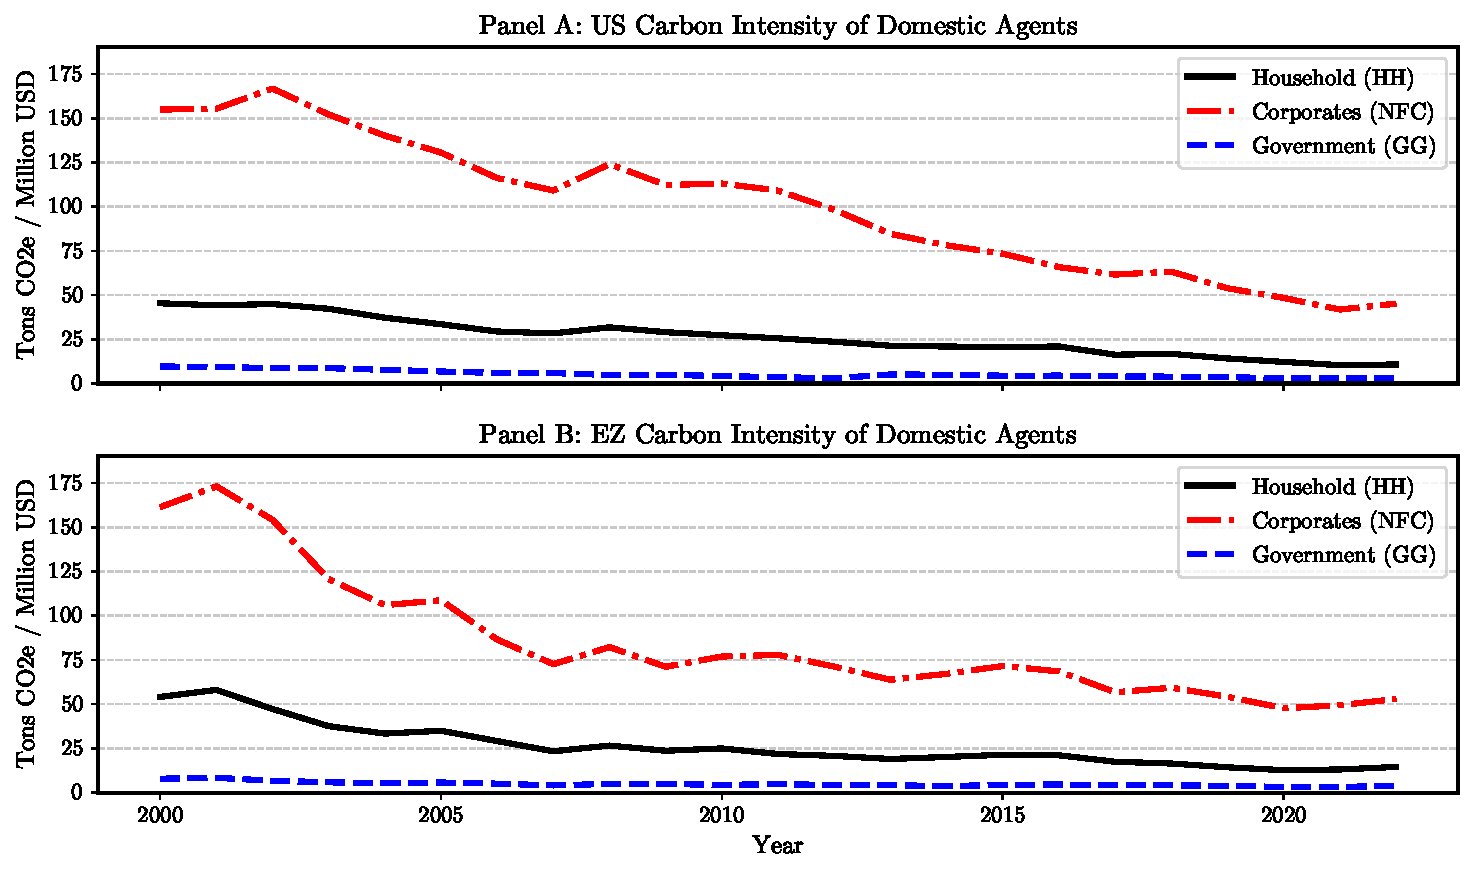
\includegraphics[width=1\textwidth]{Figures/Compare_Domestic_Intensity.pdf}
    \caption{Carbon Intensity of Domestic Agents}
    \label{fig:intensity_dom}
\end{figure}

Figure \ref{fig:intensity_row} presents the carbon intensity of the Rest of the World sector. To assess the robustness of these estimates, I construct alternative regional coverage scenarios: RoW1 corresponds to developed economies (including Europe, North America, and the Japan-Pacific region); RoW2 incorporates emerging economies with available claim information from the OECD (Brazil, India, Mexico, Russia, and Türkiye); and RoW3 expands this coverage to include China, reflecting its leading global position in both financial claims and total emissions.

For both the US and the EZ, the inclusion of emerging economies (RoW2) increases the RoW carbon intensity by approximately 20 $\text{tCO}_2\text{e}$ per million USD, while the further addition of China (RoW3) adds an additional 20 $\text{tCO}_2\text{e}$ per million USD. This disproportionate increase suggests that despite its massive debt levels, China's relative emissions remain exceptionally high. Consequently, financial institutions whose foreign exposures are concentrated in developed countries will benefit from lower portfolio carbon intensities, whereas those diversifying into emerging markets and China will incur significantly higher financed emissions. By 2022, the RoW3 carbon intensity for both the US and EZ reached approximately 60 $\text{tCO}_2\text{e}$ per million USD, ultimately surpassing the intensity of domestic non-financial corporations (NFCs) in both regions.

\begin{figure}[h]
    \centering
    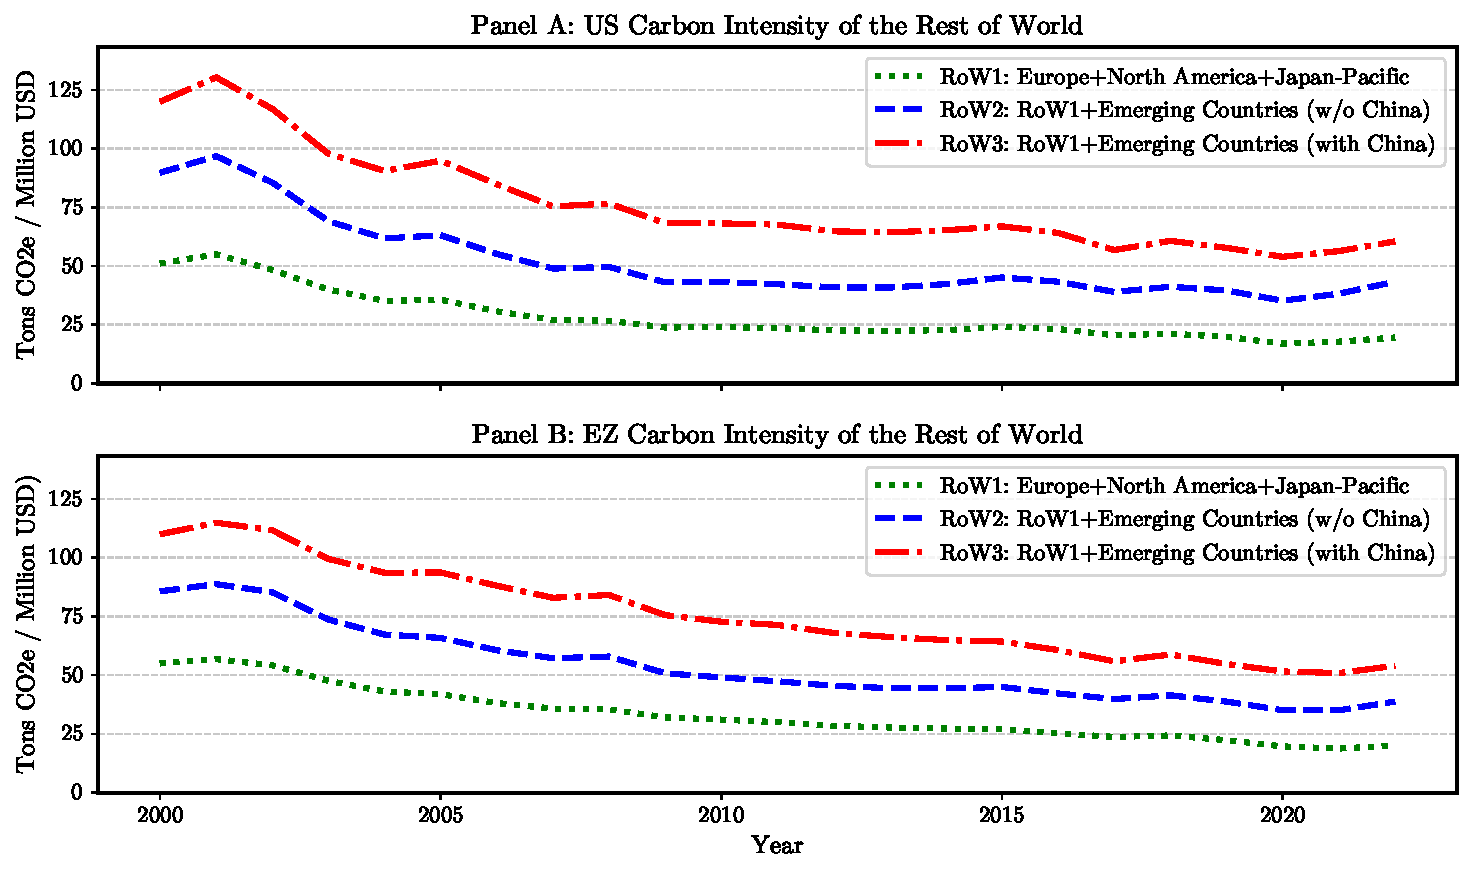
\includegraphics[width=1\textwidth]{Figures/Compare_RoW_Intensity.pdf}
    \caption{Carbon Intensity of the Rest of World}
    \label{fig:intensity_row}
\end{figure}

\subsection{System-wide financed emissions}

Figure \ref{fig:total_financed_emis} summarizes total financed emissions of the US and the Euro area across alternative RoW scenarios. The definition of RoW regions has a sizeable impact on total financed emissions, particularly for financial systems with larger foreign exposures, such as the Euro area.

The US, with its larger financial system and higher domestic corporate carbon intensity prior to 2015, initially accounts for higher financed emissions. After 2015, however, the gap narrows as foreign exposures become increasingly important. Under the broadest RoW3 scenario, which includes emerging markets and China, Euro area financed emissions surpass those of the US in recent years.

Taking RoW1 as the base-case scenario, where foreign exposures are restricted to developed markets, total financed emissions reach $2,946.8$ million tCO$_2$e for the US and $2,739.9$ million tCO$_2$e for the Euro area. Under RoW3, these estimates increase to $3,761.5$ million tCO$_2$e and $4,082.4$ million tCO$_2$e, respectively. This corresponds to an increase of approximately 28\% for the US and 49\% for the Euro area relative to RoW1, highlighting the stronger sensitivity of Euro area financed emissions to assumptions about foreign-market exposure.

These differences depend on the extent to which financing flows spill over into more carbon-intensive emerging markets and China. According to a publication by the Federal Reserve, U.S. residents' holdings of emerging market long-term securities account for approximately one-third of their total foreign holdings of long-term securities\footnote{Source: The Federal Reserve, available at \url{https://www.federalreserve.gov/releases/efa/international-portfolio-investment-figure4.pdf}}. Conversely, as noted in a keynote by \textcite{lane_euro_2024}, the Euro area maintained a relatively low allocation to emerging market equities between 2019 and 2023. Although the region had a substantial allocation to emerging market debt between 2020 and 2021, this exposure declined to insignificant levels thereafter.
 
\begin{figure}[h]
    \centering
    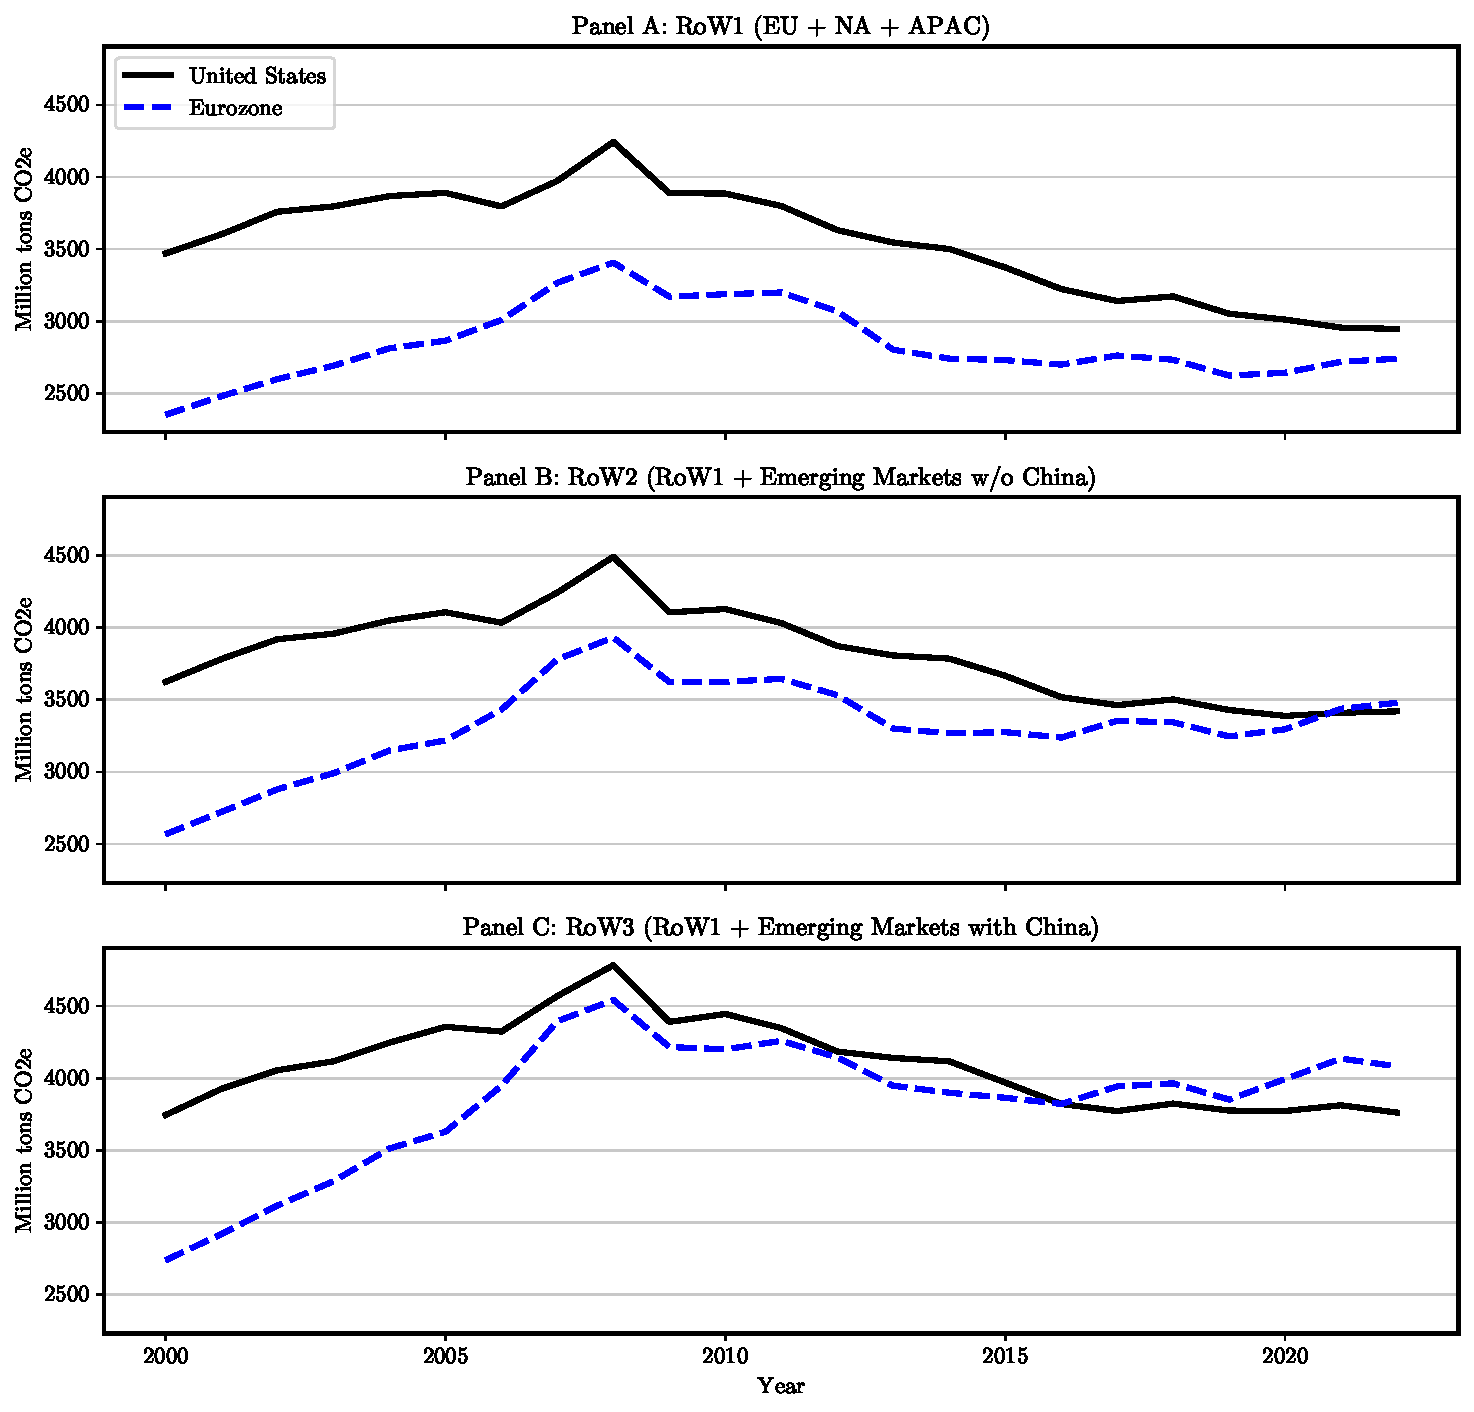
\includegraphics[width=1\textwidth]{Figures/US_vs_EU_By_Scenario_Vertical.pdf}
    \caption{Total financed emissions by RoW scenarios}
    \label{fig:total_financed_emis}
\end{figure}

Figure \ref{fig:total_financed_emis_fi} illustrates the breakdown of financed emissions across different types of financial institutions under the RoW1 scenario. Similar decompositions for the RoW2 and RoW3 scenarios are provided in the Appendix \ref{Appendix E:FE_by_FI}. The time-series patterns are broadly consistent across the three scenarios, suggesting that the relative evolution of financial institution groups is not sensitive to the choice of RoW allocation. The main difference is a vertical shift in the level of financed emissions: RoW2 and RoW3 generate higher estimates because they attribute a larger share of exposures to more carbon-intensive regions, particularly emerging markets and China. Thus, the alternative RoW assumptions primarily affect the scale of financed emissions, while leaving the composition and dynamics across financial institutions largely unchanged.

Consistent with the patterns identified in Figure \ref{fig:total_exp_fi}, the data indicates that structural market differences governing asset holdings serve as the primary driver of total financed emissions. A key observation is that investment funds account for the largest share of emissions in the US, stemming from their growing financial exposure to the domestic corporate sector. Conversely, in the Eurozone, Other Financial Institutions (OFIs) have generated emission levels comparable to those of Monetary Financial Institutions (MFIs) over the past decade, despite MFIs maintaining a significantly larger asset base. This parity is also largely driven by OFIs' increasing capital allocation toward emission-intensive non-financial corporations.
 
\begin{figure}[h]
    \centering
    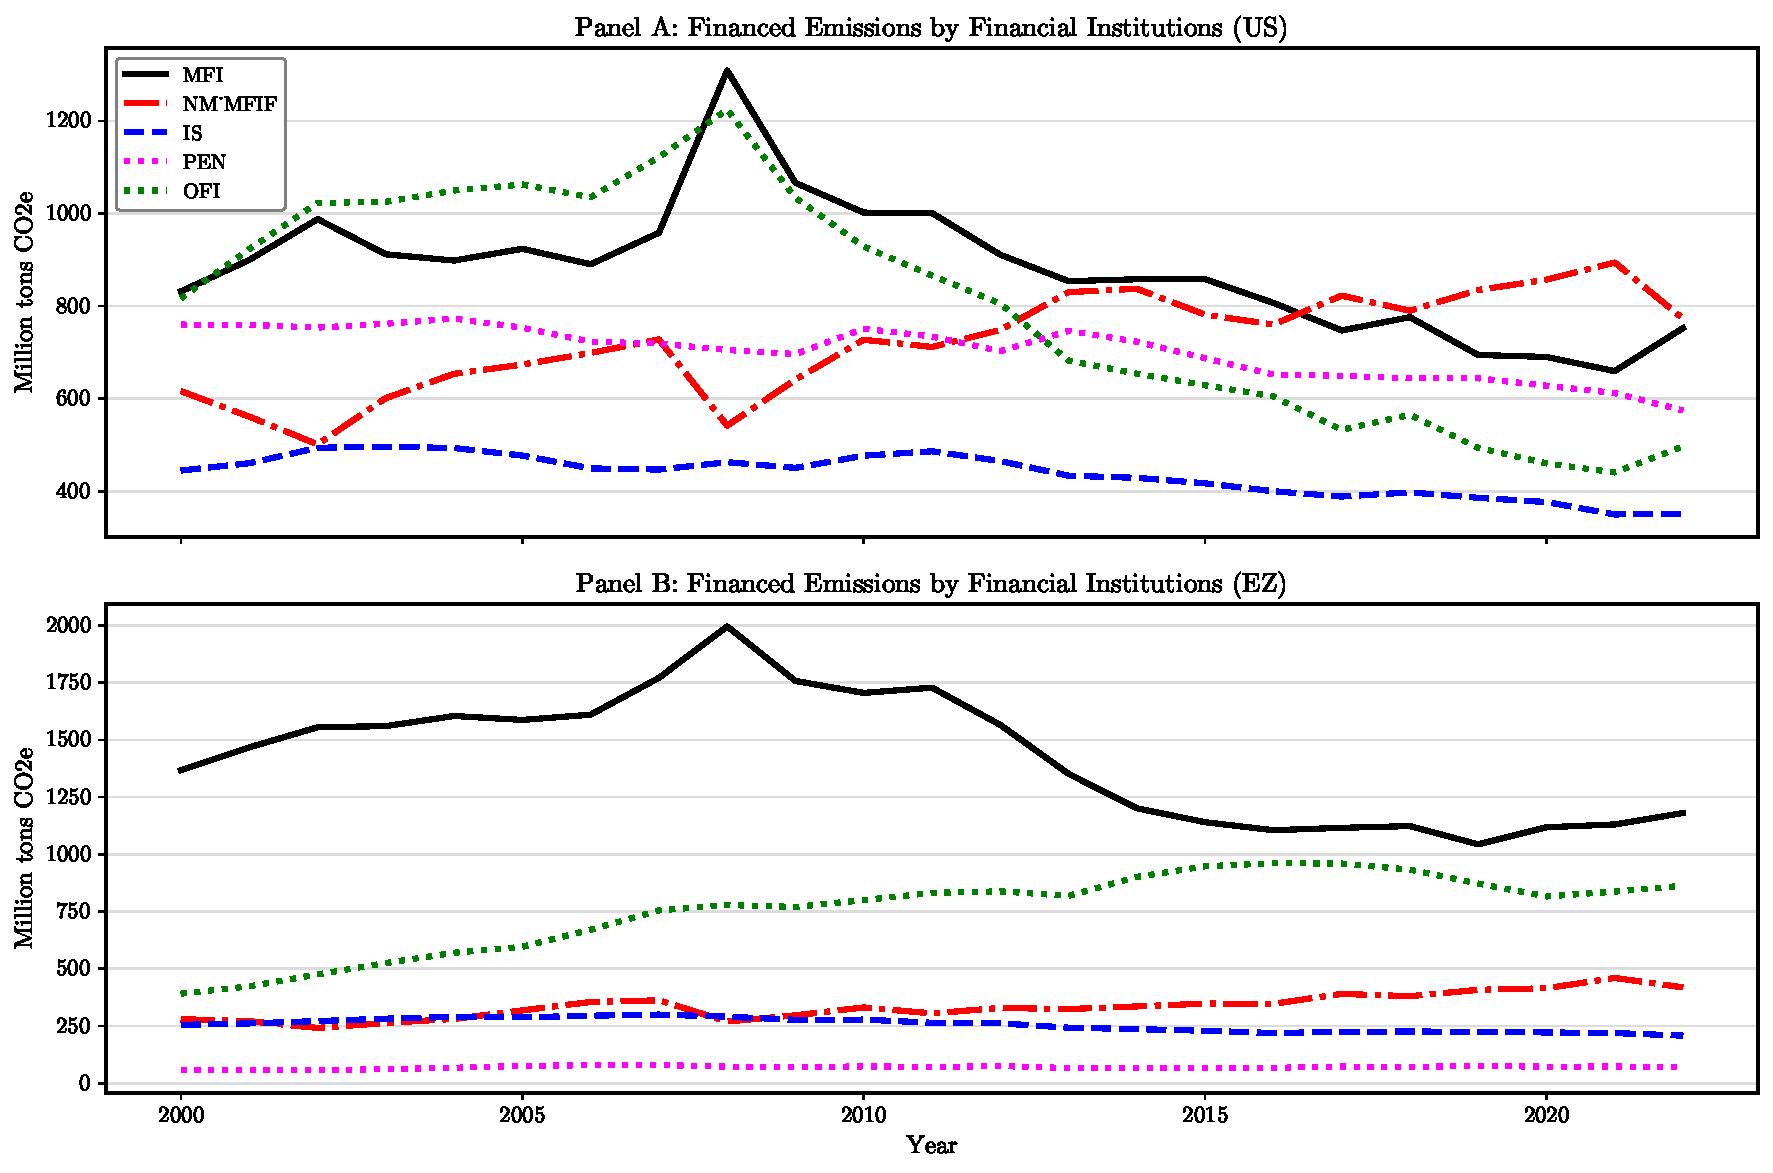
\includegraphics[width=1\textwidth]{Figures/FE_by_Institutions_RoW1.pdf}
    \caption{Total financed emissions by financial institution groups (RoW1)}
    \label{fig:total_financed_emis_fi}
\end{figure}

Figure~\ref{fig:total_financed_emis_agent} breaks down total financed GHG emissions by real-economy agents. The data reveals a profound structural divergence between the asset allocation strategies and environmental footprints of the two regions. The emissions profile of the United States financial system is characterized by an intense domestic focus and a steady long-term decline. Financed emissions are structurally dominated by domestic corporations, matching the US market-based framework where large capital-funded pension and investment fund structures allocate capital heavily into domestic securities markets. Total financed emissions have steadily contracted from their 2008 peak of approximately 3,083 million tonnes $\text{CO}_2\text{e}$. Furthermore, the cross-border layers ($\text{RoW1}$, $\text{RoW2}$, and $\text{RoW3}$) remain tight and visually compressed at the top of the stack, implying that the overall carbon footprint of the US financial sector is highly sensitive to domestic corporate decarbonization rather than international portfolio rebalancing.

In contrast, the Euro area panel exposes a structural migration of financed environmental pressures from domestic to cross-border domains. Following the dual shocks of the 2008 Global Financial Crisis and the 2012 Eurozone sovereign debt crisis, the financed emissions footprint of domestic European corporations contracted. However, this domestic compression was systematically offset by an aggressive expansion of cross-border claims. 

As the analytical lens moves sequentially from developed foreign portfolios ($\text{RoW1}$) to emerging markets ($\text{RoW2}$) and ultimately integrates China ($\text{RoW3}$), the Eurozone's total portfolio emissions experience a massive vertical shift. This visual transformation strongly supports the hypothesis that the Euro area financial system has actively outsourced its ecological footprint; driven by internal regulatory and monetary pressures, European financial intermediaries executed an international search for yield that has anchored European capital to highly carbon-intensive production networks abroad.

\begin{figure}[h]
    \centering
    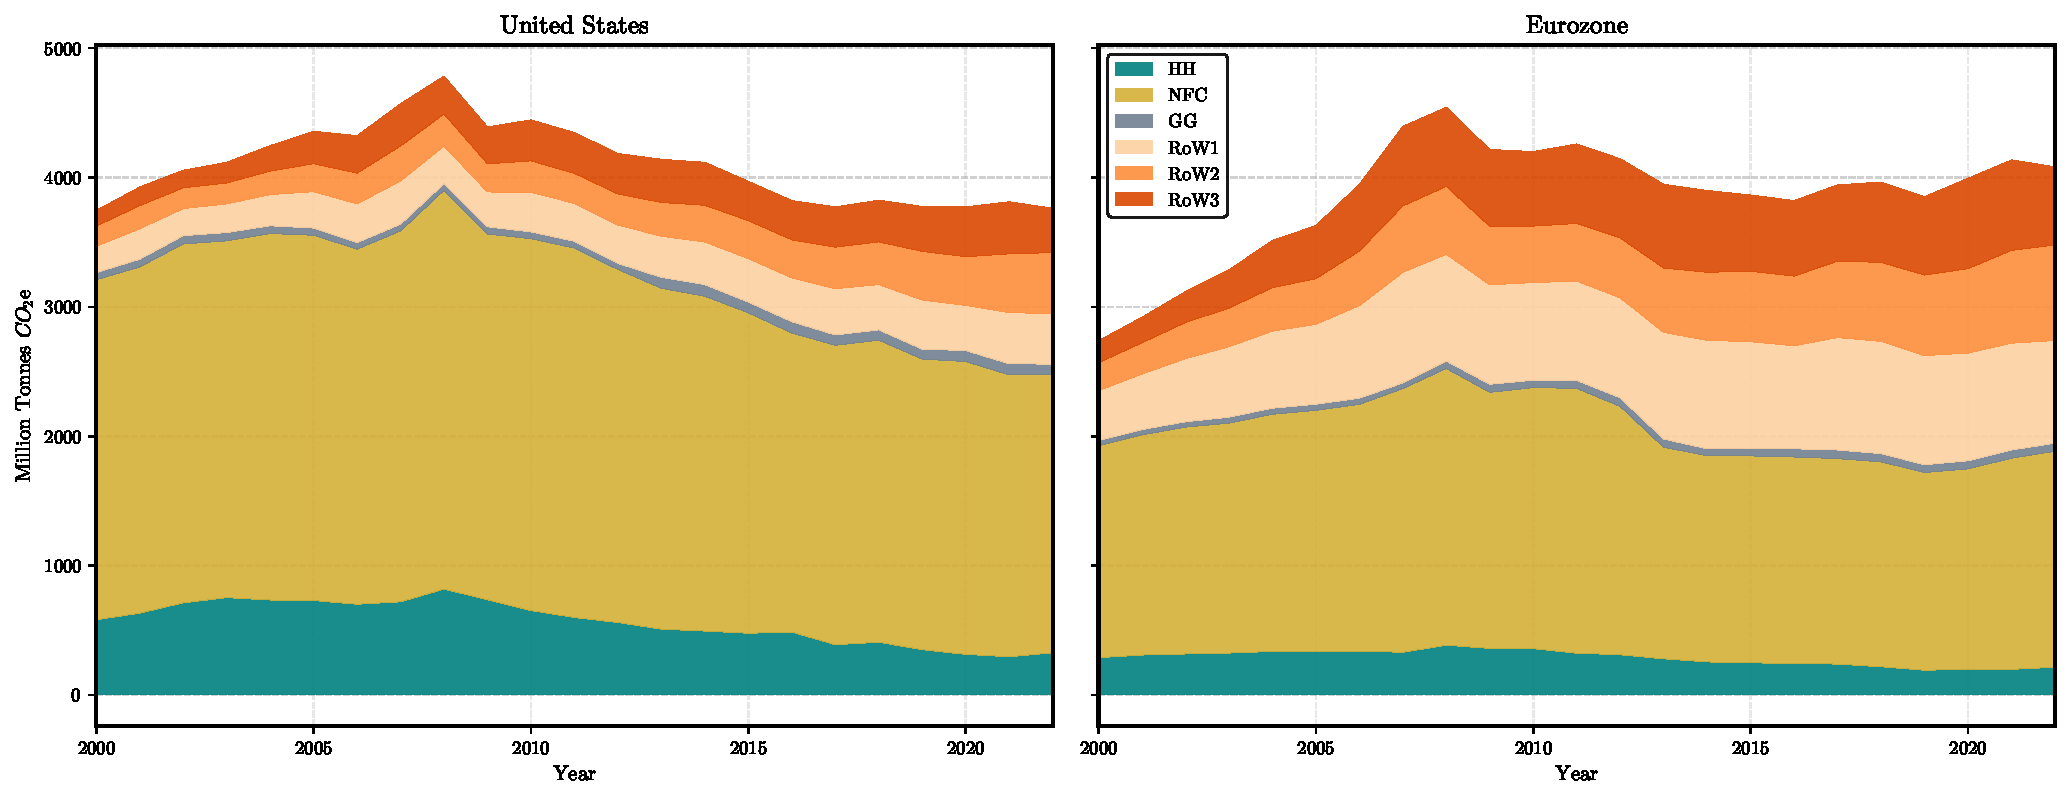
\includegraphics[width=1\textwidth]{Figures/FE_by_Agent.pdf}
    \caption{Total financed emissions by real-economy agents}
    \label{fig:total_financed_emis_agent}
\end{figure}

Figure \ref{fig:fe_cba_pba} compares the range of financed emissions (across three RoW scenarios), against two standard accounting benchmarks: production-based emissions and consumption-based emissions. PBA reflects emissions generated directly by domestic production activities within a territory, whereas CBA captures the global emissions driven by domestic final demand. Over the last two decades, PBA and CBA in both the US and the Eurozone have experienced a decline, though the reduction has been minimal. However, the absolute magnitude of emissions in the US is substantially higher, nearly double that of the Eurozone. While this partly reflects economic scale, it also suggests the US lags behind the Eurozone in its decarbonization trajectory. Furthermore, CBA consistently exceeds PBA in both regions, indicating a net importation of carbon embodied in foreign goods and services.
\begin{figure}[h]
    \centering
    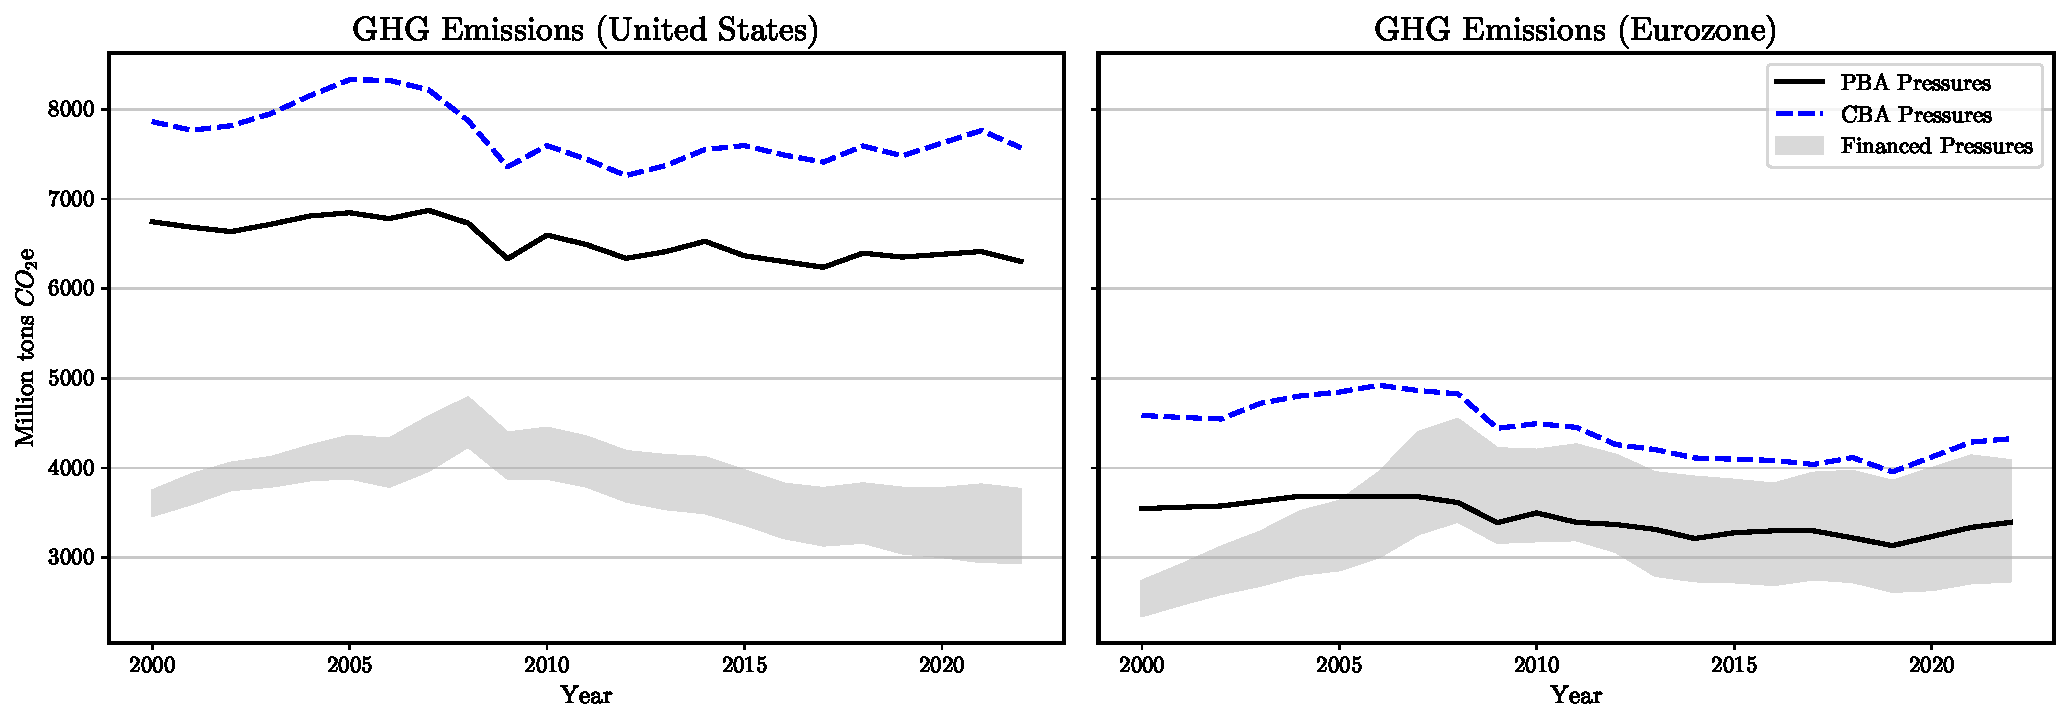
\includegraphics[width=1\textwidth]{Figures/Combined_FE_vs_PBA_CBA_GHG_emissions_GWP100_IPCC2010.pdf}
    \caption{Financed emissions in comparison with production-based and consumption-based emissions}
    \label{fig:fe_cba_pba}
\end{figure}

Interestingly, the relative significance of financed emissions diverges sharply between the two economies. In the US, although absolute financed emissions are substantial, they represent a smaller fraction of the overall carbon profile compared to massive domestic physical emissions. Conversely, in the Eurozone, the estimated range of financed emissions is roughly equivalent to the region's entire territorial (PBA) and demand-driven (CBA emissions. This highlights the disproportionately large global carbon footprint of the European financial sector relative to its domestic real economy.

\section{Other environmental pressures and resource use}
\label{sec:6.3}

In this section, the analysis is extended to other environmental pressures directly linked to the production activities enabled by financial system in the US and the Eurozone. Specifically, I consider land use, water consumption and the extraction of key material resources. The objective is to quantify how financial exposures translate into primary physical pressures on ecosystems and natural resources. 

\subsection{Land use and water consumption}

According to \textcite{stadler_exiobase_2018}, EXIOBASE considers three land-use categories: cropland, grazing land, and forestland. Cropland captures land used for crop production, grazing land refers to land used for pasture and livestock-related activities, and forestland captures land associated with forestry and timber-related production. In this thesis, the term ''land use'' refers to the aggregate of these three categories, representing the overall land-related pressure associated with economic activity.

Figure \ref{fig:land_use} compares production-based, consumption-based, and financed land-use pressures for the United States and the Eurozone. In both regions, consumption-based pressures are consistently higher than production-based pressures, suggesting that domestic consumption relies on land-intensive production outside the domestic economy. The United States exhibits substantially larger land-use pressures than the Eurozone across all accounting approaches. For the United States, financed land-use pressures remain relatively stable below both PBA and CBA measures. In contrast, financed land-use pressures in the Eurozone are closer to domestic production-based pressures and exceed them for most of the sample period. This indicates that, while Eurozone territorial land-use pressures are relatively limited, its financial system is associated with a broader land-use footprint through cross-border financial exposures. Overall, the figure highlights that financial-system-based accounting provides a distinct perspective from both production- and consumption-based measures, especially for economies with different financial structures and international exposure patterns.

\begin{figure}[h]
    \centering
    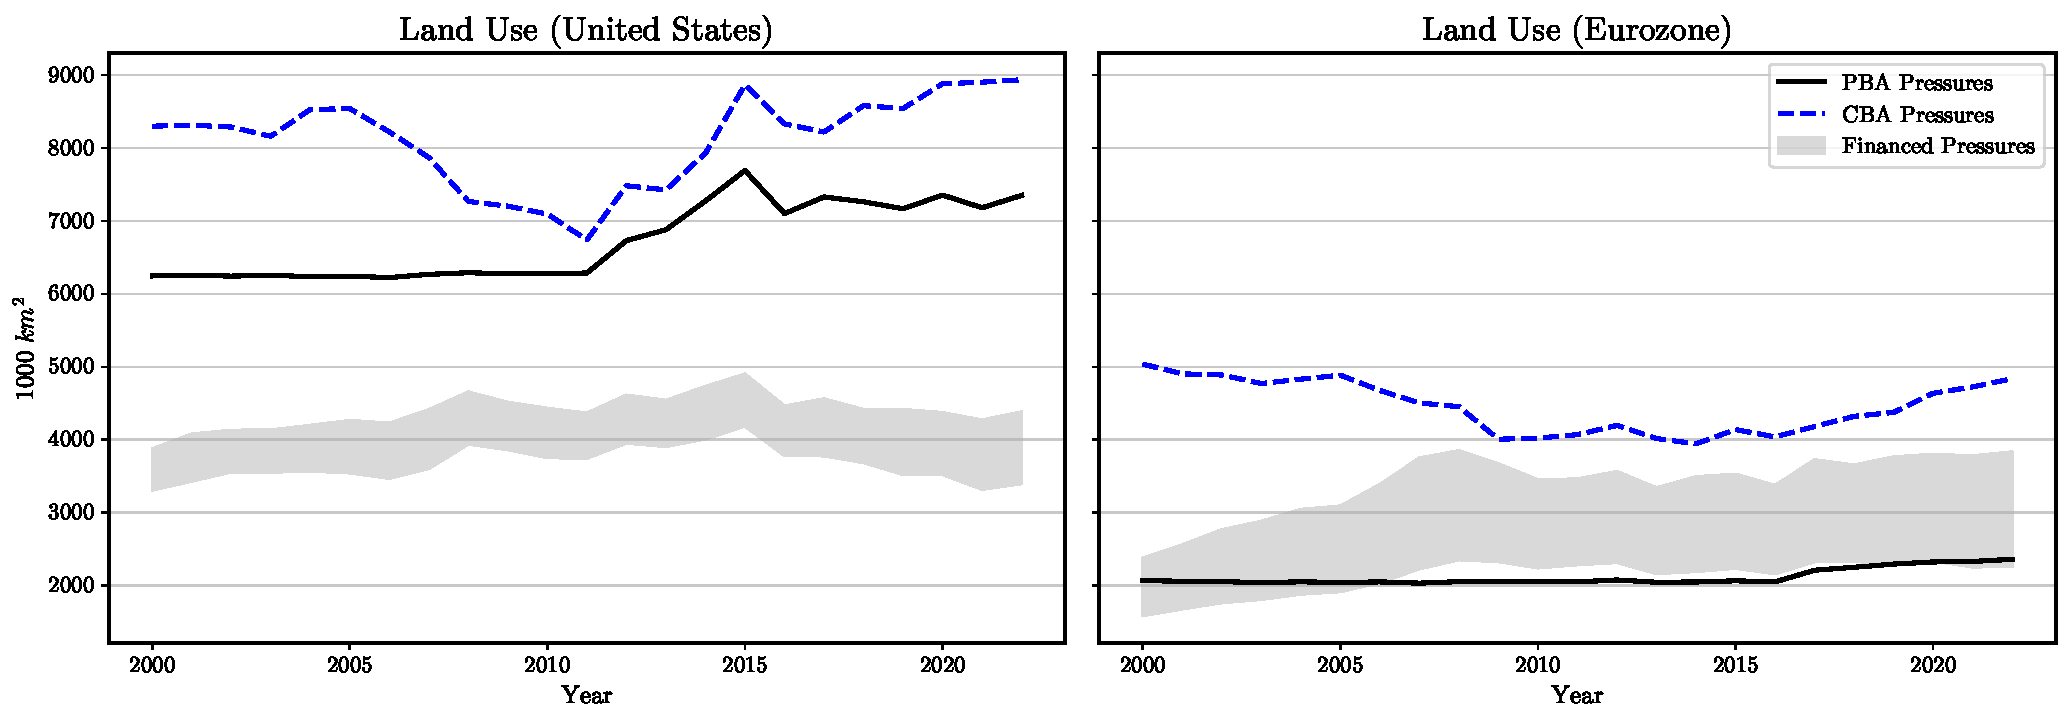
\includegraphics[width=1\textwidth]{Figures/Combined_FE_vs_PBA_CBA_Land_use_Crop_Forest_Pasture.pdf}
    \caption{Financed pressures in comparison with production-based and consumption-based pressures (Land Use in 1000 $km^2$)}
    \label{fig:land_use}
\end{figure}

Water-related accounts in EXIOBASE distinguish between green and blue water, as well as between water withdrawal and water consumption. The hydrological cycle is composed of both blue and green water. Blue water refers to the share of precipitation that flows into aquifers, lakes, rivers, and other surface-water and groundwater resources \citep{savenije_water_2000}. It is the main source of water for human needs, industrial production, and irrigated agriculture \citep{dantas_economic_2021}. Green water refers to the part of precipitation that is intercepted by vegetation, stored in the soil, transpired back to the atmosphere, or temporarily available for vegetation growth \citep{quinteiro_contribution_2015}. It plays a central role in agricultural production and is estimated to support around 60--70\% of global food production \citep{rost_agricultural_2008}.

Water withdrawal refers to the amount of water removed from natural sources and allocated to human activities \citep{gleick_water_2003, rijsberman_water_2006}. However, part of the withdrawn water may return to the natural water system before or after production processes. By contrast, water consumption refers to the portion of water that is consumed during production or use and does not return to the same hydrological system. Compared with water withdrawal, water consumption therefore provides a closer measure of water depletion and of the effective environmental pressure placed on freshwater resources. In this thesis, water pressure is measured using total blue water consumption, which aggregates blue water consumed across the main EXIOBASE activity categories, including agriculture, livestock production, electricity generation, manufacturing, and domestic use.

Figure \ref{fig:water_use} compares production-based, consumption-based, and financed pressures for total blue water consumption. In both the United States and the Euro area, consumption-based pressures exceed production-based pressures, indicating that both economies are net importers of blue-water consumption through international trade. However, the size of this gap differs substantially across the two regions. In the United States, CBA and PBA pressures remain relatively close to each other throughout the sample period, suggesting that foreign embodied water use plays a more limited role relative to domestic water consumption. By contrast, the Euro area shows a much larger and more persistent gap: production-based pressures remain relatively stable at around 40 billion m$^3$, while consumption-based pressures are roughly twice as large. This indicates that the Euro area relies more heavily on water-intensive production taking place outside its own territorial boundary.

The role of financed water pressures also differs between the two financial systems. In the United States, financed pressures remain clearly below both PBA and CBA measures, implying that financial-system exposures account for a relatively smaller share of the economy's overall blue-water footprint. In the Euro area, financed pressures are much closer to consumption-based pressures and rise above both PBA and CBA measures towards the end of the sample. This suggests that, compared with the United States, the Euro area financial system is more strongly linked to water-intensive real-economy activities through cross-border financial claims. Overall, the figure shows that both economies are net importers of water pressure, but the external dependence is more pronounced for the Euro area, where financial exposures also play a more important role in shaping the aggregate water footprint.

\begin{figure}[h]
    \centering
    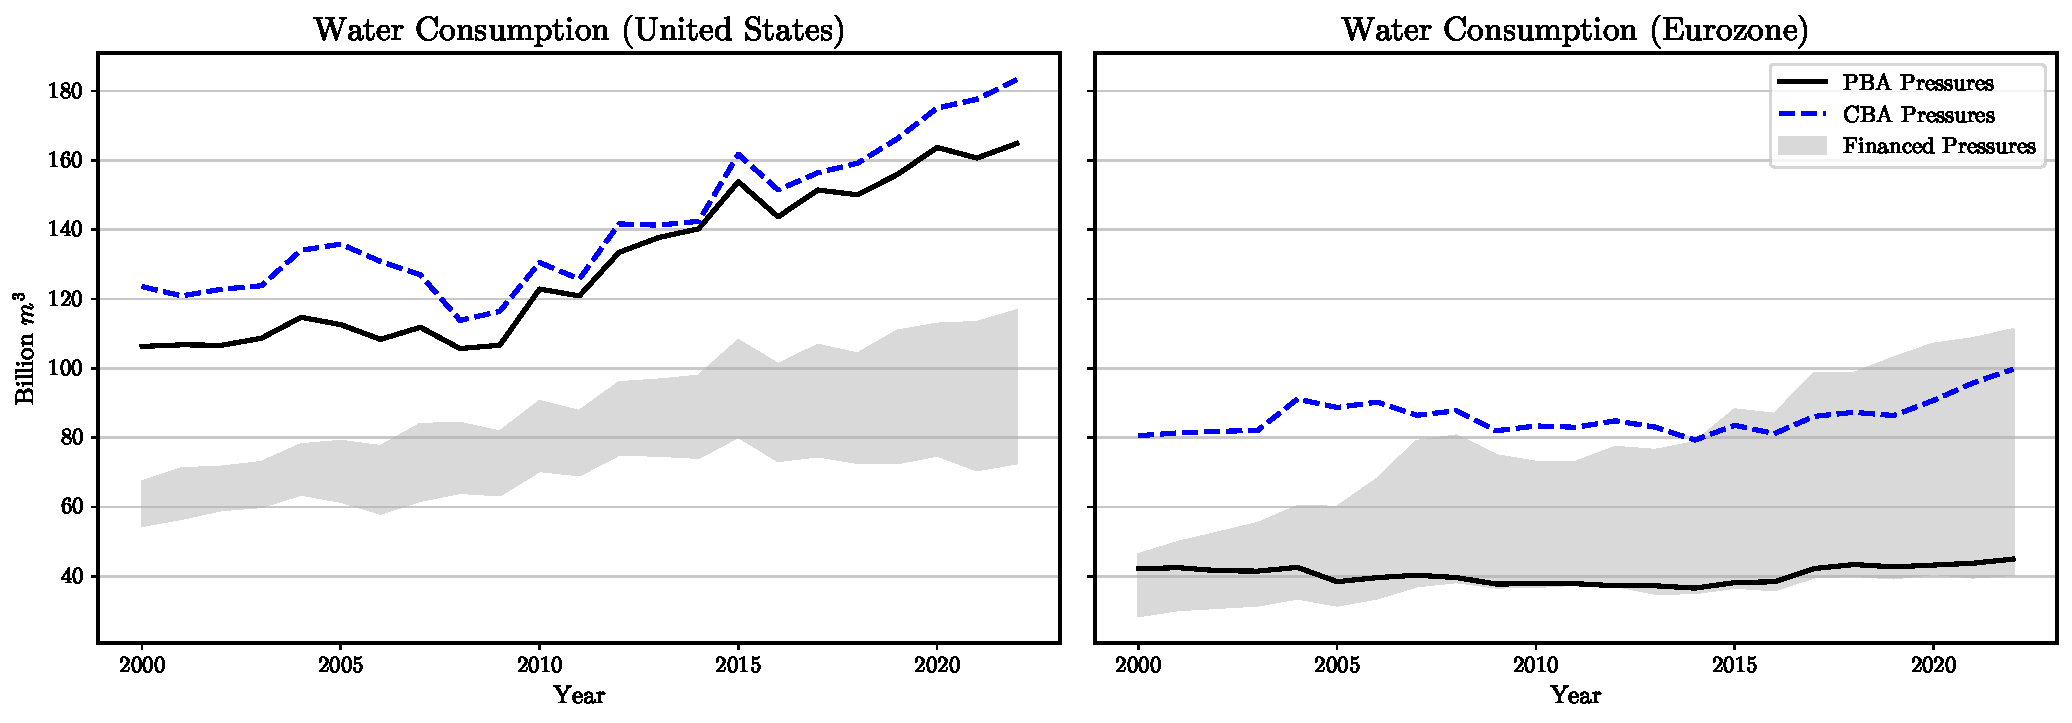
\includegraphics[width=1\textwidth]{Figures/Combined_FE_vs_PBA_CBA_Water_Consumption_Blue_Total.pdf}
    \caption{Financed pressures in comparison with production-based and consumption-based pressures (Water Consumption in billions $m^3$)}
    \label{fig:water_use}
\end{figure}

\subsection{Resource Extraction}

Resource extraction provides another dimension of environmental pressure associated with economic activity. In EXIOBASE, material extraction includes fossil fuels, iron ore, non-ferrous metal ores, and non-metallic minerals. These resources are tightly linked to different segments of the global production system. Fossil fuels are closely related to primary energy consumption, electricity generation, and carbon-intensive manufacturing processes. Iron ore serves as the foundational upstream raw material required for global steel production, linking it directly to heavy industrial manufacturing, machinery fabrication, and large-scale engineering projects. Non-ferrous metal ores, such as copper and aluminum, represent critical inputs for advanced engineering, electronics, and specialized industrial supply chains. Finally, non-metallic minerals, including sand, gravel, and limestone, are largely consumed by construction and infrastructure-related activities. Unlike GHG emissions, which measure an undesirable output of production, resource extraction captures the upstream, primary physical material requirements needed to sustain economic production and consumption.

Figure \ref{fig:resource_extraction_all} compares production-based, consumption-based, and financed pressures for four categories of resource extraction. Across most categories, consumption-based pressures exceed production-based pressures, indicating that both the United States and the Euro area rely on material extraction embodied in imported goods and foreign production chains. However, this dependence is more pronounced for the Euro area. In the United States, domestic extraction remains relatively important, especially for fossil fuels and non-metallic minerals, so the gap between production-based and consumption-based pressures is generally moderate. By contrast, the Euro area displays a larger and more systematic gap between consumption-based and production-based pressures, particularly for fossil fuels, non-ferrous metal ores, and iron ore. This suggests that the Euro area's material footprint is more strongly shaped by extraction taking place outside its territorial boundary.

The financed-pressure measure further highlights the difference between the two financial systems. In the United States, financed resource-extraction pressures generally remain below production-based and consumption-based pressures, suggesting that financial-system exposures play a relatively smaller role in the US material footprint. In the Euro area, financed pressures are closer to consumption-based pressures and often exceed production-based pressures, especially for metal ores. This indicates that Euro area financial institutions are linked to resource-intensive activities that largely take place abroad. Overall, the figure shows that both economies are net importers of material pressures through trade, but the external dependence is stronger for the Euro area. 

\begin{figure}[htbp]
    \centering
    \begin{tabular}{c}
        % ==================== CHART 1 ====================
        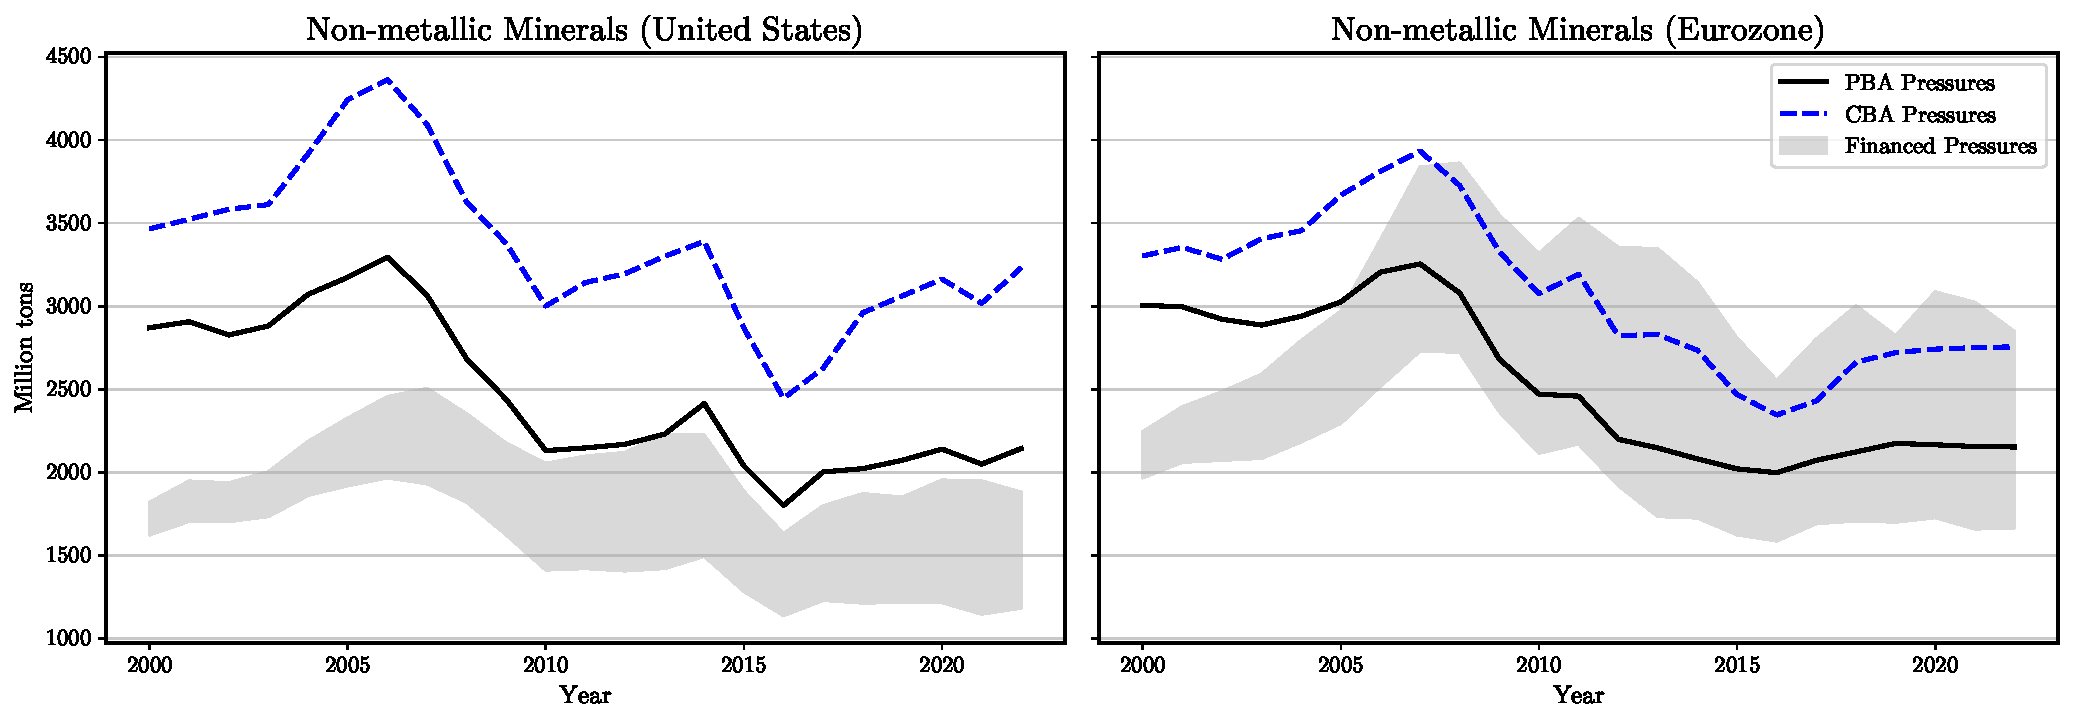
\includegraphics[width=0.9\textwidth]{Figures/Combined_FE_vs_PBA_CBA_DEU_Non_metalic_Minerals.pdf}\\
        
        % ==================== CHART 2 ====================
        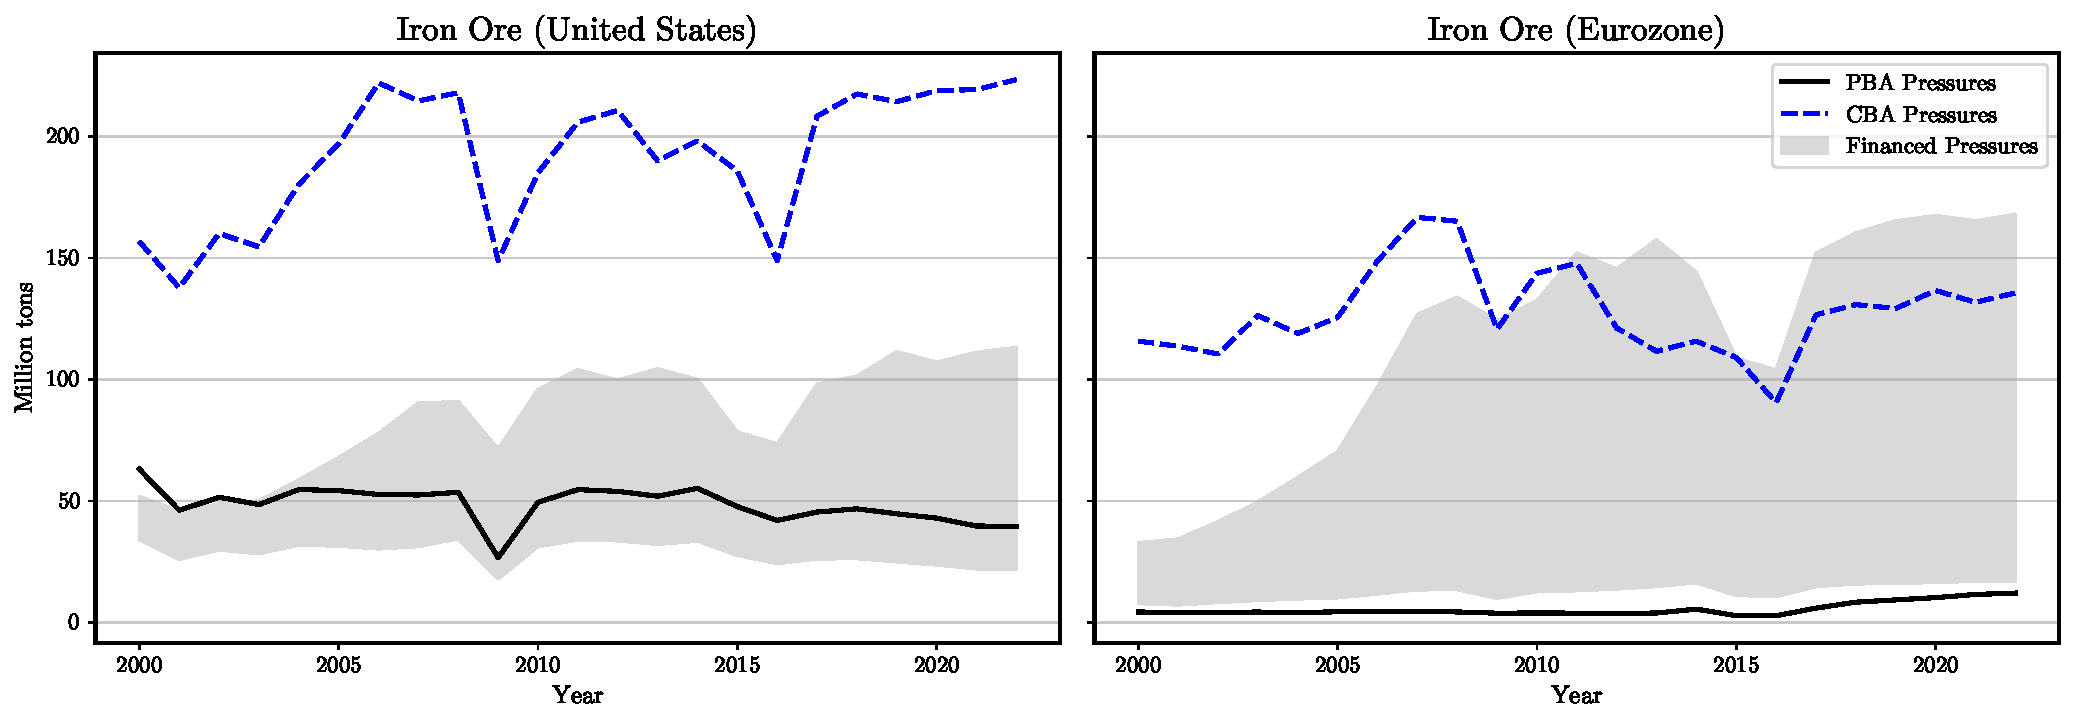
\includegraphics[width=0.9\textwidth]{Figures/Combined_FE_vs_PBA_CBA_DEU_Iron_Ore.pdf} \\
        
        % ==================== CHART 3 ====================
        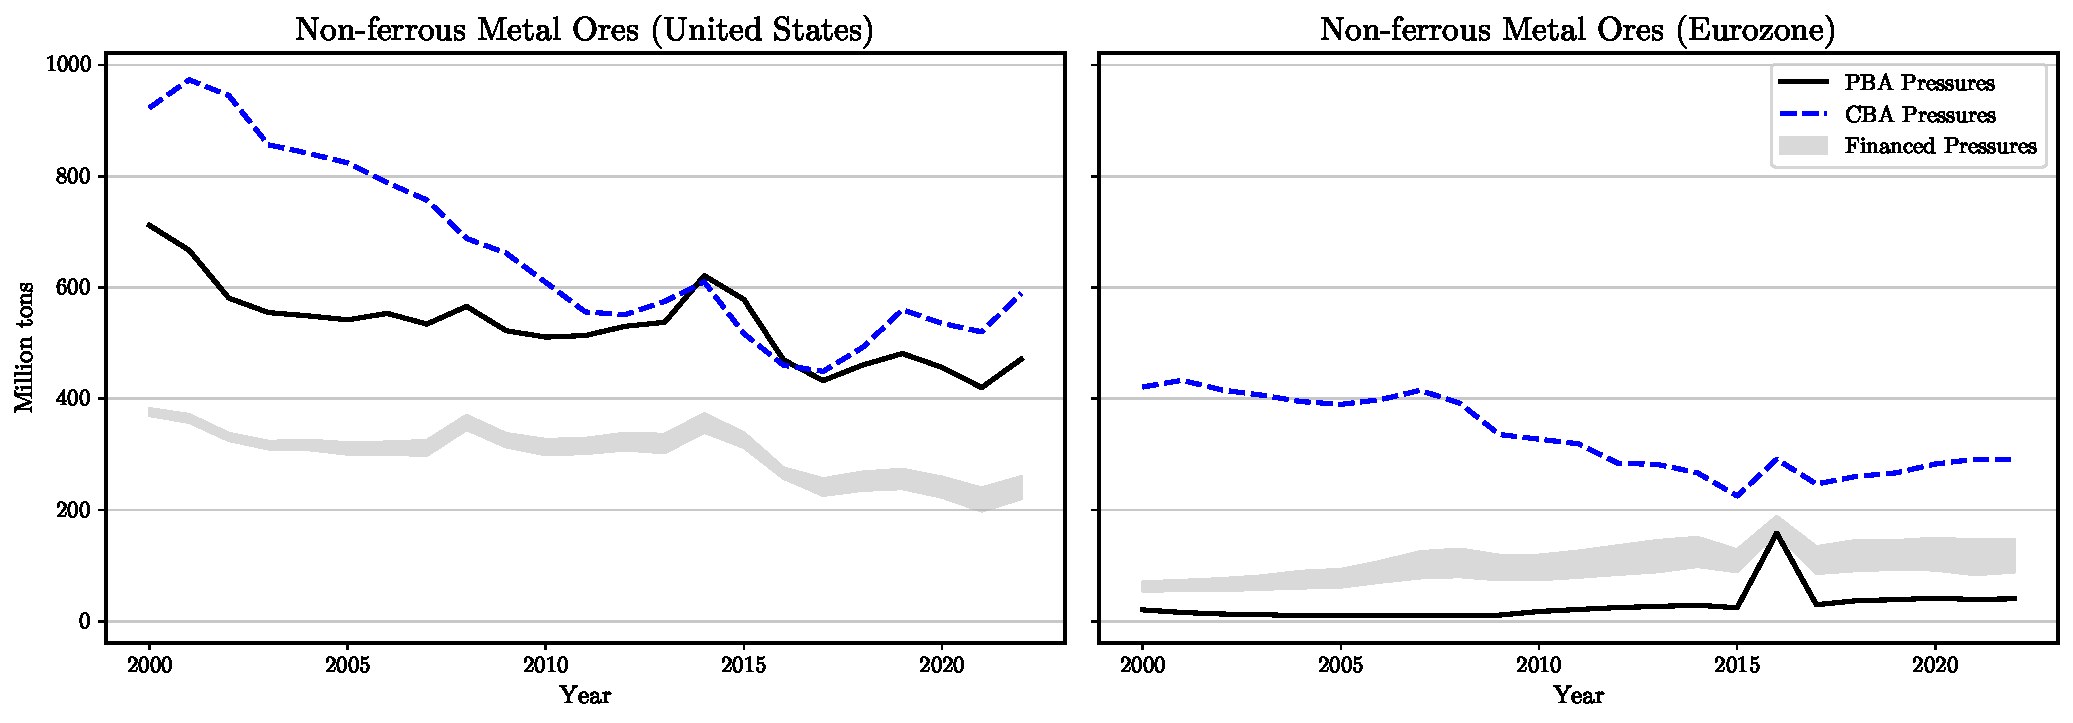
\includegraphics[width=0.9\textwidth]{Figures/Combined_FE_vs_PBA_CBA_DEU_Non_ferous_metal_ores.pdf} \\
        
        % ==================== CHART 4 ====================
        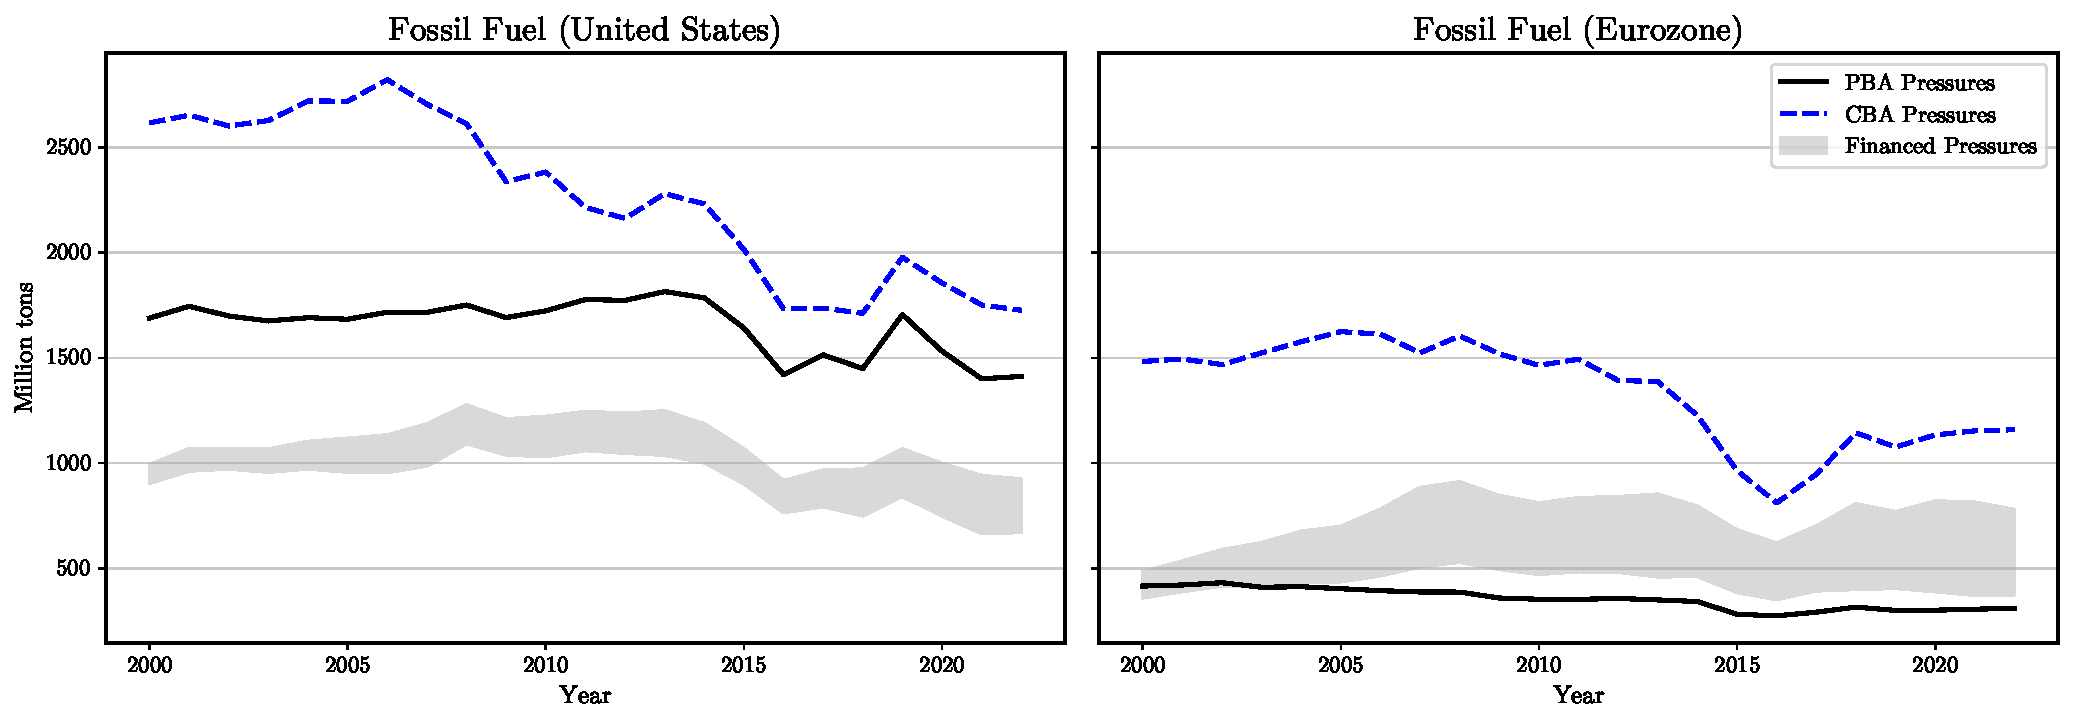
\includegraphics[width=0.9\textwidth]{Figures/Combined_FE_vs_PBA_CBA_DEU_Fossil_Fuel.pdf} \\
    \end{tabular}

    % ==================== MAIN CAPTION ====================
    \caption{Financed pressures in comparison with production-based and consumption-based pressures for Resource Extraction variants (Physical Units in Million tons).}
    \label{fig:resource_extraction_all}
\end{figure} 
% Chapter 7

\chapter{Conclusion} % Main chapter title

\label{Chapter7} % For referencing the chapter elsewhere, use \ref{Chapter7} 

\section{Summary of Empirical Findings}

This thesis has applied a comprehensive macroeconomic framework developed by \textcite{jondeau_environmental_2026} to quantify and compare the global environmental pressures linked to the financial systems of the United States and the Euro area from 2000 to 2022. By integrating national financial accounts with the environmentally extended multi-regional input-output (EE-MRIO) database EXIOBASE v3, the analysis yields three central insights regarding the structural differences, geographical spillovers, and multi-dimensional footprints of major macro-financial systems.

First, the empirical results confirm that structural domestic differences determine the channels through which environmental pressures are financed. In the United States, a fundamentally market-based system, financed emissions are heavily concentrated within investment and pension funds, reflecting their substantial capital allocation toward domestic non-financial corporations (NFCs). Conversely, the Euro area’s bank-based framework routes its environmental impacts primarily through traditional Monetary Financial Institutions (MFIs) and specialized Other Financial Institutions (OFIs) that increasingly finance emitters across borders. 

Second, a stark divergence has emerged in the geographical footprint of the two financial regimes. While the US financial system has consistently maintained an inward focus, allocating over 80\% of its exposure to domestic sectors, the Euro area financial system has increasingly become an engine for cross-border financing. Driven by post-2012 structural dynamics, including the stagnation of internal sovereign debt financing linked to the bank-sovereign "doom loop" and an extended period of negative interest rate policies, Euro area institutions aggressively expanded their foreign claims. By 2022, the Rest of the World (RoW) sector accounted for approximately 40\% of the Euro area's total exposure. 

Third, this outward allocation means that the Euro area has effectively "outsourced" its environmental footprint. When emerging markets and China are incorporated into the investment pool (the RoW3 scenario), the Euro area's financed emissions surpass those of the US in recent years. Remarkably, while absolute financed emissions in the US represent a smaller fraction of its massive domestic physical profile, the Euro area's financed emissions range is roughly equivalent to its entire territorial. This global footprint is not limited to carbon; the Euro area financial system exhibits an equally disproportionate external dependence on global ecosystems via cross-border claims linked to intensive land use, blue-water depletion, and upstream mineral and fossil fuel extraction.

\section{Policy Implications for Central Banks and Regulators}

The empirical findings of this thesis carry several implications for central banks, macro-prudential supervisors, and international financial standard-setters navigating the climate transition.

First, the results suggest that financial regulation can shape financed emissions in unintended ways by influencing the allocation of capital across sectors and regions. For example, Basel III liquidity rules, such as the Liquidity Coverage Ratio, may help anchor US financial capital in relatively low-carbon Treasury securities, while Euro area sovereign-risk dynamics and yield-search incentives may encourage greater exposure to more carbon-intensive foreign assets. This implies that financial stability policies should not be assessed solely through the lens of domestic risk reduction, but also in relation to their broader environmental footprint.

Second, the findings have implications for climate stress testing. Existing exercises, such as the ECB's 2022 climate risk stress test and the Federal Reserve's pilot Climate Scenario Analysis exercise, provide an important starting point for assessing climate-related financial risks at the bank level. However, because these frameworks are mainly designed around banks' exposures to clients, counterparties, and selected credit portfolios, they may be less suited to capturing macro-financial risks arising from the aggregate allocation of capital across sectors and countries. This thesis therefore highlights the value of complementing existing supervisory exercises with system-level, multi-regional approaches that account for cross-border financial intermediation and the carbon intensity of foreign assets.

Third, by extending the macro-financial framework beyond greenhouse gas emissions to land use, water consumption, and resource extraction, this thesis speaks to the broader principle of double materiality. Environmental risks are not limited to carbon emissions: financial systems may also be exposed to physical vulnerabilities arising from water scarcity, land degradation, biodiversity loss, or resource dependence. This is particularly relevant for highly internationalized financial systems such as the Euro area, where cross-border claims may finance production networks with substantial non-carbon environmental pressures. These findings suggest that climate-related financial supervision should gradually move beyond carbon-focused metrics and incorporate a wider set of environmental indicators. More harmonized disclosure and satellite-accounting frameworks could help supervisors and financial institutions identify portfolios that appear relatively climate-aligned in terms of emissions, but remain exposed to significant environmental pressures through land, water, or resource channels.

\section{Future Research and Concluding Remarks}

One of the main assumptions of the framework is that the geographic distribution of final borrowers is not directly observed. As a result, the model assumes that financial systems fund developed economies, emerging economies, or both groups proportionally, based on each group’s claims relative to total global claims. If more granular information on the national profile of credit recipients becomes available, future research could incorporate this information to improve the accuracy of the attribution exercise.

Second, the current public coverage of EXIOBASE extends only to 2022, and the most recent years should be interpreted with caution. This highlights the need for the continued development of environmentally extended multi-regional input-output databases that combine broad country and sectoral coverage with frequent updates and detailed environmental indicators. Future work could therefore contribute to the construction of reliable and regularly updated EE-MRIO sources, particularly for applications in climate finance and macro-financial risk assessment.

Third, future research could reconcile the macroeconomic attribution framework used in this thesis with bottom-up financed-emissions measures reported by major financial institutions. Such a comparison would help assess the completeness and consistency of existing emissions and environmental-pressure disclosures, while also identifying potential gaps across institutions, asset classes, and jurisdictions.

In summary, as ecological and climate crises accelerate, the definition of a “safe” or “sustainable” financial system must undergo a fundamental shift. This thesis shows that an economy cannot achieve a genuine green transition through the decarbonization of domestic production alone if its financial intermediaries continue to enable environmental degradation across borders. Measuring sustainability purely through territorial production or final consumption metrics overlooks the structural role of globalized financial capital in shaping environmental outcomes. By adopting a comprehensive financial-environmental attribution framework, central banks, regulators, and market participants can more accurately evaluate, disclose, and ultimately mitigate the global ecosystem pressures enabled by modern financial systems.
 

%----------------------------------------------------------------------------------------
%	THESIS CONTENT - APPENDICES
%----------------------------------------------------------------------------------------


\appendix % Resets chapter counters to letters (A, B, C)

% Include the appendices of the thesis as separate files from the Appendices folder
% 1. Manually inject "Appendices" into the Table of Contents right here
\cleardoublepage
\addcontentsline{toc}{chapter}{Appendices}


% 3. Start your regular Appendix A chapter
\chapter*{Appendices}
\chapter{Structural Restrictions}
\label{Appendix A: Structural Restrictions}

% Your Appendix A content continues here...

This appendix documents the structural restriction matrices $Z^{(k)}$ applied to each
financial instrument $k$ in the construction of the FWTW matrix for the euro area.
Each matrix is a binary $(0,1)$ mask, where 1 denotes an admissible entry and 0 a
restricted one.

Rows and columns follow the harmonized institutional-sector order used in the
main analysis: monetary financial institutions, non-money market funds investment funds, insurance corporations, pension funds, other
financial institutions, households, non-financial corporations, general
government, and rest of the world.

\begingroup
\footnotesize
\setlength{\arraycolsep}{2.4pt}
\renewcommand{\arraystretch}{0.85}

\newcommand{\zmat}[2]{%
\begin{minipage}[t]{0.32\textwidth}
\centering
\textbf{\footnotesize #1}\\[2pt]
\resizebox{0.82\linewidth}{!}{$
\begin{bmatrix}
#2
\end{bmatrix}$}
\end{minipage}
}

\begin{center}

\zmat{Gold}{
1&0&0&0&0&0&0&1&1\\
0&0&0&0&0&0&0&0&0\\
0&0&0&0&0&0&0&0&0\\
0&0&0&0&0&0&0&0&0\\
0&0&0&0&0&0&0&0&0\\
0&0&0&0&0&0&0&0&0\\
0&0&0&0&0&0&0&0&0\\
0&0&0&0&0&0&0&0&0\\
1&0&0&0&0&0&0&1&0
}
\hfill
\zmat{Currency}{
1&0&0&0&0&0&0&0&1\\
1&0&0&0&0&0&0&0&1\\
1&0&0&0&0&0&0&0&1\\
1&0&0&0&0&0&0&0&1\\
1&0&0&0&0&0&0&0&1\\
1&0&0&0&0&0&0&0&1\\
1&0&0&0&0&0&0&0&1\\
1&0&0&0&0&0&0&0&1\\
1&0&0&0&0&0&0&0&0
}
\hfill
\zmat{Debt Instruments}{
1&1&1&0&1&0&1&1&1\\
1&1&1&1&1&0&1&1&1\\
1&1&1&1&1&0&1&1&1\\
1&1&1&0&1&0&1&1&1\\
1&1&1&1&1&0&1&1&1\\
1&1&1&0&1&0&1&1&1\\
1&1&1&0&1&0&1&1&1\\
1&1&1&0&1&0&1&1&1\\
1&1&1&0&1&0&1&1&0
}

\vspace{10pt}

\zmat{Listed Shares}{
1&1&1&0&1&0&1&1&1\\
1&1&1&0&1&0&1&1&1\\
1&1&1&0&1&0&1&1&1\\
1&1&1&0&1&0&1&1&1\\
1&1&1&0&1&0&1&1&1\\
1&1&1&0&1&0&1&1&1\\
1&1&1&0&1&0&1&1&1\\
1&1&1&0&1&0&1&1&1\\
1&1&1&0&1&0&1&1&0
}
\hfill
\zmat{Unlisted Shares}{
1&0&1&0&1&0&1&0&1\\
1&0&1&0&1&0&1&1&1\\
1&0&1&0&1&0&1&0&1\\
1&0&1&0&1&0&1&1&1\\
1&1&1&1&1&0&1&1&1\\
1&0&1&0&1&0&1&0&1\\
1&0&1&0&1&0&1&1&1\\
1&0&1&0&1&0&1&1&1\\
1&0&1&0&1&0&1&1&0
}
\hfill
\zmat{Other Equity}{
1&0&1&0&1&0&1&0&1\\
1&0&1&0&1&0&1&1&1\\
1&0&1&0&1&0&1&0&1\\
1&0&1&0&1&0&1&1&1\\
1&1&1&1&1&0&1&1&1\\
1&0&1&0&1&0&1&0&1\\
1&0&1&0&1&1&1&1&1\\
1&0&1&0&1&0&1&1&1\\
1&0&1&0&1&0&1&1&0
}

\vspace{10pt}

\zmat{Money Market Fund Shares}{
1&0&0&0&0&0&0&0&1\\
1&0&0&0&0&0&0&0&1\\
1&0&0&0&0&0&0&0&1\\
1&0&0&0&0&0&0&0&1\\
1&0&0&0&0&0&0&0&1\\
1&0&0&0&0&0&0&0&1\\
1&0&0&0&0&0&0&0&1\\
1&0&0&0&0&0&0&0&1\\
1&0&0&0&0&0&0&0&0
}
\hfill
\zmat{Mutual Fund Shares}{
0&1&0&0&0&0&0&0&1\\
0&1&0&0&0&0&0&0&1\\
0&1&0&0&0&0&0&0&1\\
0&1&0&0&0&0&0&0&1\\
0&1&0&0&0&0&0&0&1\\
0&1&0&0&0&0&0&0&1\\
0&1&0&0&0&0&0&0&1\\
0&1&0&0&0&0&0&0&1\\
0&1&0&0&0&0&0&0&0
}
\hfill
\zmat{Life Insurance}{
0&0&0&0&0&0&0&0&0\\
0&0&0&0&0&0&0&0&0\\
0&0&0&0&0&0&0&0&0\\
0&0&1&1&0&0&0&0&0\\
0&0&0&0&0&0&0&0&0\\
0&0&1&1&0&0&0&0&0\\
0&0&1&1&0&0&0&0&0\\
0&0&0&0&0&0&0&0&0\\
0&0&0&0&0&0&0&0&0
}

\vspace{10pt}

\zmat{Non-Life Insurance}{
1&1&1&1&1&0&0&1&0\\
1&1&1&1&1&0&0&1&0\\
1&1&1&1&1&0&0&1&0\\
1&1&1&1&1&0&0&1&0\\
1&1&1&1&1&0&0&1&0\\
1&1&1&1&1&0&0&1&0\\
1&1&1&1&1&0&0&1&0\\
1&1&1&1&1&0&0&1&0\\
0&0&0&0&0&0&0&0&0
}
\hfill
\zmat{Pension Schemes}{
1&0&1&1&1&1&1&1&0\\
0&0&0&0&0&0&0&0&0\\
1&0&1&1&1&1&1&1&0\\
1&0&1&1&1&1&1&1&0\\
1&0&1&1&1&1&1&1&0\\
1&0&1&1&1&1&1&1&0\\
1&0&1&1&1&1&1&1&0\\
1&0&1&1&1&1&1&1&0\\
0&0&0&0&0&0&0&0&0
}
\hfill
\zmat{Other}{
1&1&1&1&1&1&1&1&1\\
1&1&1&1&1&1&1&1&1\\
1&1&1&1&1&1&1&1&1\\
1&1&1&1&1&1&1&1&1\\
1&1&1&1&1&1&1&1&1\\
1&1&1&1&1&1&1&1&1\\
1&1&1&1&1&1&1&1&1\\
1&1&1&1&1&1&1&1&1\\
1&1&1&1&1&1&1&1&0
}

\end{center}

\endgroup
\chapter{Total Discrepancies}
\label{Appendix B:Total_dis}

This appendix reports the magnitude of discrepancies (DIS) as a percentage of total
issuance for the United States and the Euro area over the 2000-2022 period.
Discrepancies are defined as the difference between total lending and borrowing
across all asset classes.

These results justify excluding discrepancies from the main analysis, as their
share of total issuance remains small and therefore does not materially affect
the effective exposure measures.

\vspace{5pt}

\begin{table}[h]
\centering
\caption{Discrepancies as a percentage of total issuance}
\label{tab:dis_us_eu}
\begin{tabular}{lcc}
\toprule
Year & United States (\%) & Euro Area (\%) \\
\midrule
2000 & 1.187 & 0.437 \\
2001 & 1.424 & 0.456 \\
2002 & 1.372 & 0.473 \\
2003 & 0.999 & 0.449 \\
2004 & 1.030 & 0.414 \\
2005 & 1.426 & 0.461 \\
2006 & 2.226 & 0.463 \\
2007 & 2.521 & 0.478 \\
2008 & 2.407 & 0.526 \\
2009 & 2.115 & 0.619 \\
2010 & 0.882 & 0.789 \\
2011 & 1.071 & 0.869 \\
2012 & 1.079 & 0.858 \\
2013 & 0.530 & 0.645 \\
2014 & 0.664 & 0.666 \\
2015 & 0.579 & 0.616 \\
2016 & 0.505 & 0.650 \\
2017 & 0.930 & 0.623 \\
2018 & 1.102 & 0.619 \\
2019 & 1.819 & 0.709 \\
2020 & 2.282 & 0.747 \\
2021 & 1.757 & 0.691 \\
2022 & 2.543 & 0.735 \\
\bottomrule
\end{tabular}
\end{table}
\chapter{Country Coverage and Regional Classifications}
\label{Appendix C:Countries}


This appendix details the geographical scope and structural mapping of the data used in our analysis. It provides a comprehensive breakdown of the 44 countries sourced from the EXIOBASE3 and OECD Financial Accounts databases. For each country, the table indicates its broader regional grouping (Europe, North America, Asia-Pacific, or Emerging Markets) and its status as a Eurozone member state. Furthermore, it explicitly defines the composition of the ``Rest of the World'' ($RoW$) attribution base, marking exactly which countries are included when calculating foreign claims relative to the United States and the Euro area home regions.

% [Insert the \begin{longtable} code here]
\begingroup
\footnotesize % Smaller font size (one step down from \small)
\setlength{\tabcolsep}{3pt} % Tighter horizontal space between columns
\renewcommand{\arraystretch}{0.8} % Tighter vertical space between rows

% Column specs: 
% 1. p{2.0cm} -> Region (wraps text, slightly narrower for smaller font)
% 2. l        -> Country (left-aligned)
% 3-7. c      -> Checkmark columns (centered)
\begin{longtable}{>{\raggedright\arraybackslash}p{2.0cm} l c c c c c}
\toprule
\textbf{Region} & \textbf{Country} & \textbf{EXIOBASE3} & \textbf{OECD} & \textbf{Eurozone} & \textbf{RoW - US} & \textbf{RoW - Eurozone} \\
\midrule[1pt]
\endfirsthead

% Header for subsequent pages (if the table breaks across pages)
\toprule
\textbf{Region} & \textbf{Country} & \textbf{EXIOBASE3} & \textbf{OECD} & \textbf{Eurozone} & \textbf{RoW - US} & \textbf{RoW - Eurozone} \\
\midrule[1pt]
\endhead

% Footer for pages that break
\midrule
\endfoot

% Footer for the very end of the table
\bottomrule
\endlastfoot

& \textit{Total Count} & \textit{44} & \textit{42} & \textit{20} & \textit{36} & \textit{19} \\
\midrule[1pt] % Thick line to start the data

% --- EUROPE ---
Europe & Austria & \checkmark & \checkmark & \checkmark & \checkmark & \\ \cmidrule(l){2-7}
& Belgium & \checkmark & \checkmark & \checkmark & \checkmark & \\ \cmidrule(l){2-7}
& Bulgaria & \checkmark & \checkmark & & \checkmark & \checkmark \\ \cmidrule(l){2-7}
& Croatia & \checkmark & \checkmark & \checkmark & \checkmark & \\ \cmidrule(l){2-7}
& Cyprus & \checkmark & & \checkmark & & \\ \cmidrule(l){2-7}
& Czechia & \checkmark & \checkmark & & \checkmark & \checkmark \\ \cmidrule(l){2-7}
& Denmark & \checkmark & \checkmark & & \checkmark & \checkmark \\ \cmidrule(l){2-7}
& Estonia & \checkmark & \checkmark & \checkmark & \checkmark & \\ \cmidrule(l){2-7}
& Finland & \checkmark & \checkmark & \checkmark & \checkmark & \\ \cmidrule(l){2-7}
& France & \checkmark & \checkmark & \checkmark & \checkmark & \\ \cmidrule(l){2-7}
& Germany & \checkmark & \checkmark & \checkmark & \checkmark & \\ \cmidrule(l){2-7}
& Greece & \checkmark & \checkmark & \checkmark & \checkmark & \\ \cmidrule(l){2-7}
& Hungary & \checkmark & \checkmark & & \checkmark & \checkmark \\ \cmidrule(l){2-7}
& Ireland & \checkmark & \checkmark & \checkmark & \checkmark & \\ \cmidrule(l){2-7}
& Italy & \checkmark & \checkmark & \checkmark & \checkmark & \\ \cmidrule(l){2-7}
& Latvia & \checkmark & \checkmark & \checkmark & \checkmark & \\ \cmidrule(l){2-7}
& Lithuania & \checkmark & \checkmark & \checkmark & \checkmark & \\ \cmidrule(l){2-7}
& Luxembourg & \checkmark & \checkmark & \checkmark & \checkmark & \\ \cmidrule(l){2-7}
& Malta & \checkmark & & \checkmark & & \\ \cmidrule(l){2-7}
& Netherlands & \checkmark & \checkmark & \checkmark & \checkmark & \\ \cmidrule(l){2-7}
& Norway & \checkmark & \checkmark & & \checkmark & \checkmark \\ \cmidrule(l){2-7}
& Poland & \checkmark & \checkmark & & \checkmark & \checkmark \\ \cmidrule(l){2-7}
& Portugal & \checkmark & \checkmark & \checkmark & \checkmark & \\ \cmidrule(l){2-7}
& Romania & \checkmark & \checkmark & & \checkmark & \checkmark \\ \cmidrule(l){2-7}
& Slovakia & \checkmark & \checkmark & \checkmark & \checkmark & \\ \cmidrule(l){2-7}
& Slovenia & \checkmark & \checkmark & \checkmark & \checkmark & \\ \cmidrule(l){2-7}
& Spain & \checkmark & \checkmark & \checkmark & \checkmark & \\ \cmidrule(l){2-7}
& Sweden & \checkmark & \checkmark & & \checkmark & \checkmark \\ \cmidrule(l){2-7}
& Switzerland & \checkmark & \checkmark & & \checkmark & \checkmark \\ \cmidrule(l){2-7}
& United Kingdom & \checkmark & \checkmark & & \checkmark & \checkmark \\ \cmidrule(l){2-7}
& Iceland & & \checkmark & & & \\
\midrule[1pt] % THICK line separating regions

% --- NORTH AMERICA ---
North America & Canada & \checkmark & \checkmark & & \checkmark & \checkmark \\ \cmidrule(l){2-7}
& United States & \checkmark & \checkmark & & & \checkmark \\
\midrule[1pt] % THICK line separating regions

% --- ASIA PACIFIC ---
Asia-Pacific & Australia & \checkmark & & & & \\ \cmidrule(l){2-7}
& South Korea & \checkmark & \checkmark & & \checkmark & \checkmark \\ \cmidrule(l){2-7}
& Taiwan & \checkmark & & & & \\ \cmidrule(l){2-7}
& Japan & \checkmark & \checkmark & & \checkmark & \checkmark \\ \cmidrule(l){2-7}
& New Zealand & & \checkmark & & & \\
\midrule[1pt] % THICK line separating regions

% --- EMERGING MARKETS ---
Emerging Markets & Brazil & \checkmark & \checkmark & & \checkmark & \checkmark \\ \cmidrule(l){2-7}
& China & \checkmark & & & \checkmark & \checkmark \\ \cmidrule(l){2-7}
& India & \checkmark & \checkmark & & \checkmark & \checkmark \\ \cmidrule(l){2-7}
& Indonesia & \checkmark & & & & \\ \cmidrule(l){2-7}
& Mexico & \checkmark & \checkmark & & \checkmark & \checkmark \\ \cmidrule(l){2-7}
& Russia & \checkmark & \checkmark & & \checkmark & \checkmark \\ \cmidrule(l){2-7}
& South Africa & \checkmark & & & & \\ \cmidrule(l){2-7}
& Türkiye & \checkmark & \checkmark & & \checkmark & \checkmark \\ \cmidrule(l){2-7}
& Chile & & \checkmark & & & \\ \cmidrule(l){2-7}
& Colombia & & \checkmark & & & \\ \cmidrule(l){2-7}
& Israel & & \checkmark & & & \\

\end{longtable}
\endgroup
\chapter{Decomposition of Carbon Intensity}
\label{Appendix D:Decompostion}

\begin{figure}[h]
    \centering
    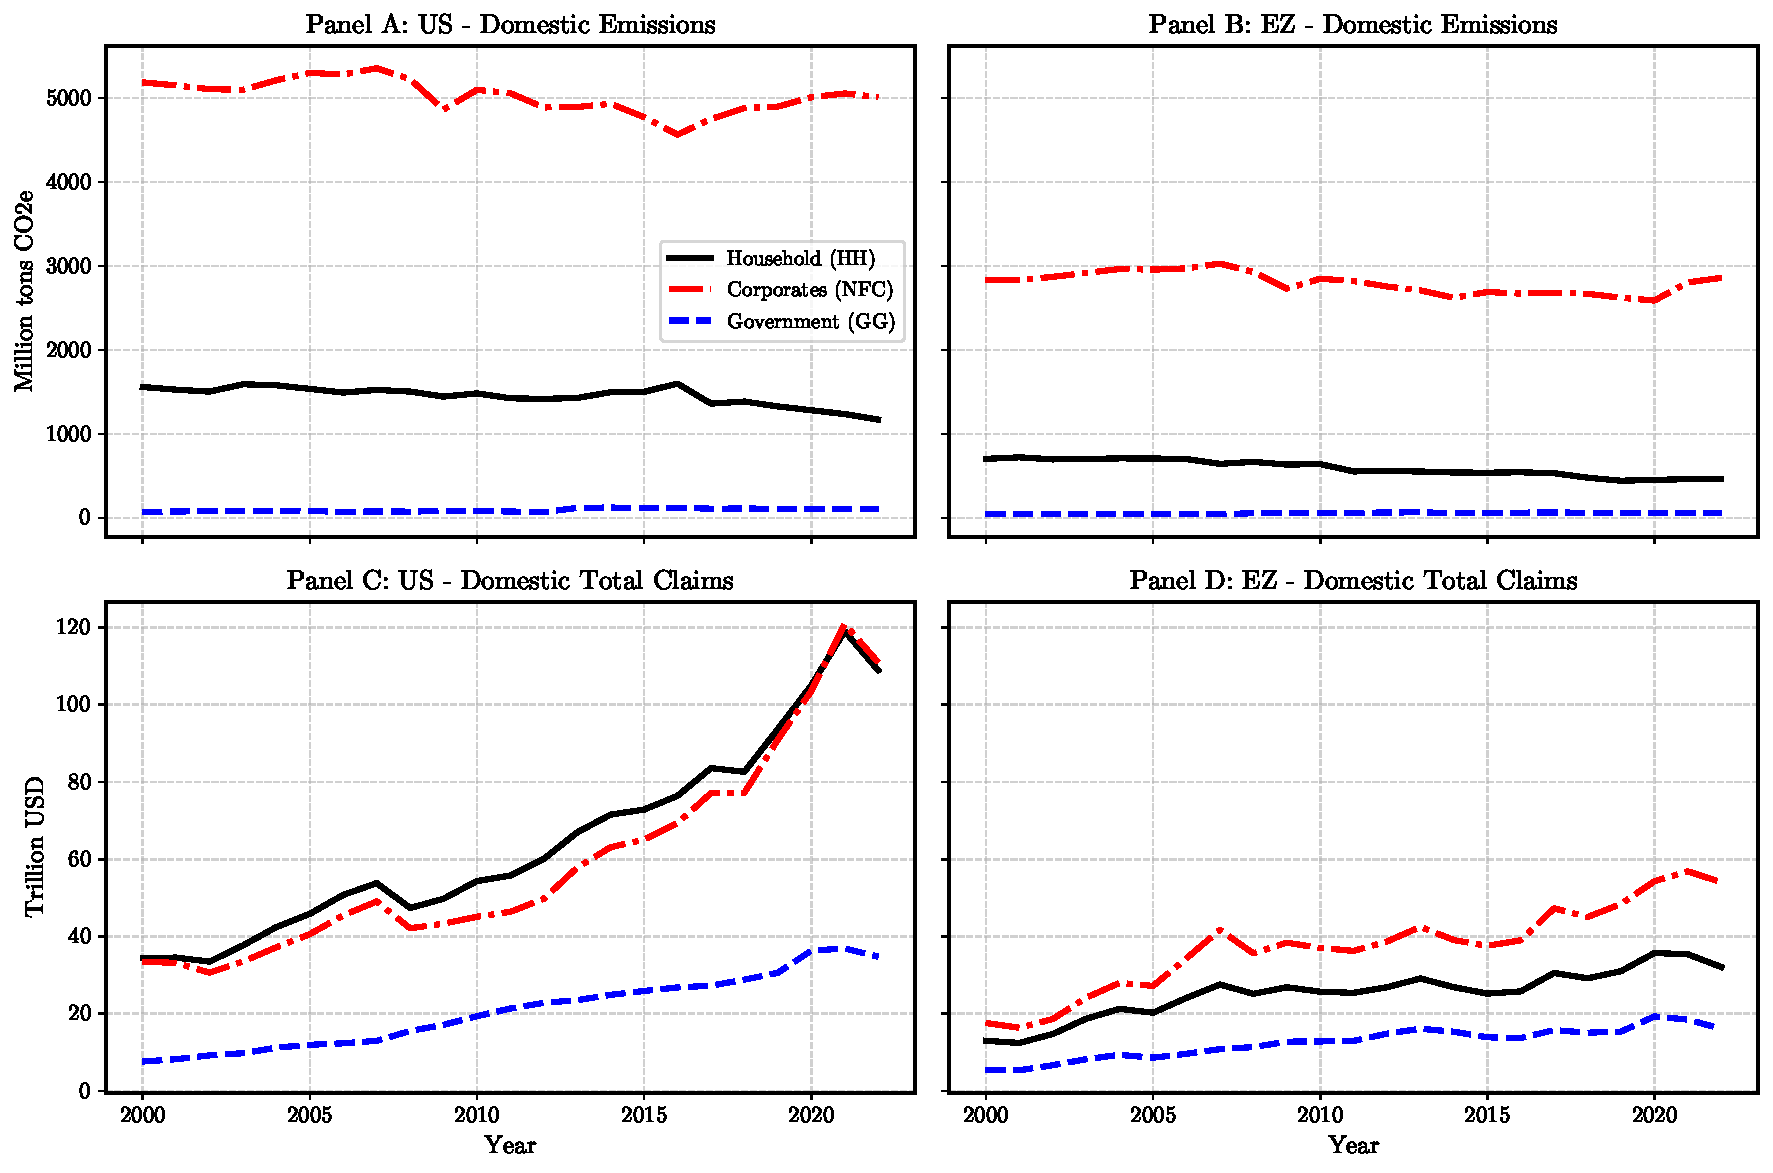
\includegraphics[width=1\textwidth]{Figures/Decomposition_Domestic.pdf}
    \caption{Decomposition of Carbon Intensity for Domestic Agents}
\end{figure}

\begin{figure}[t!]
    \centering
    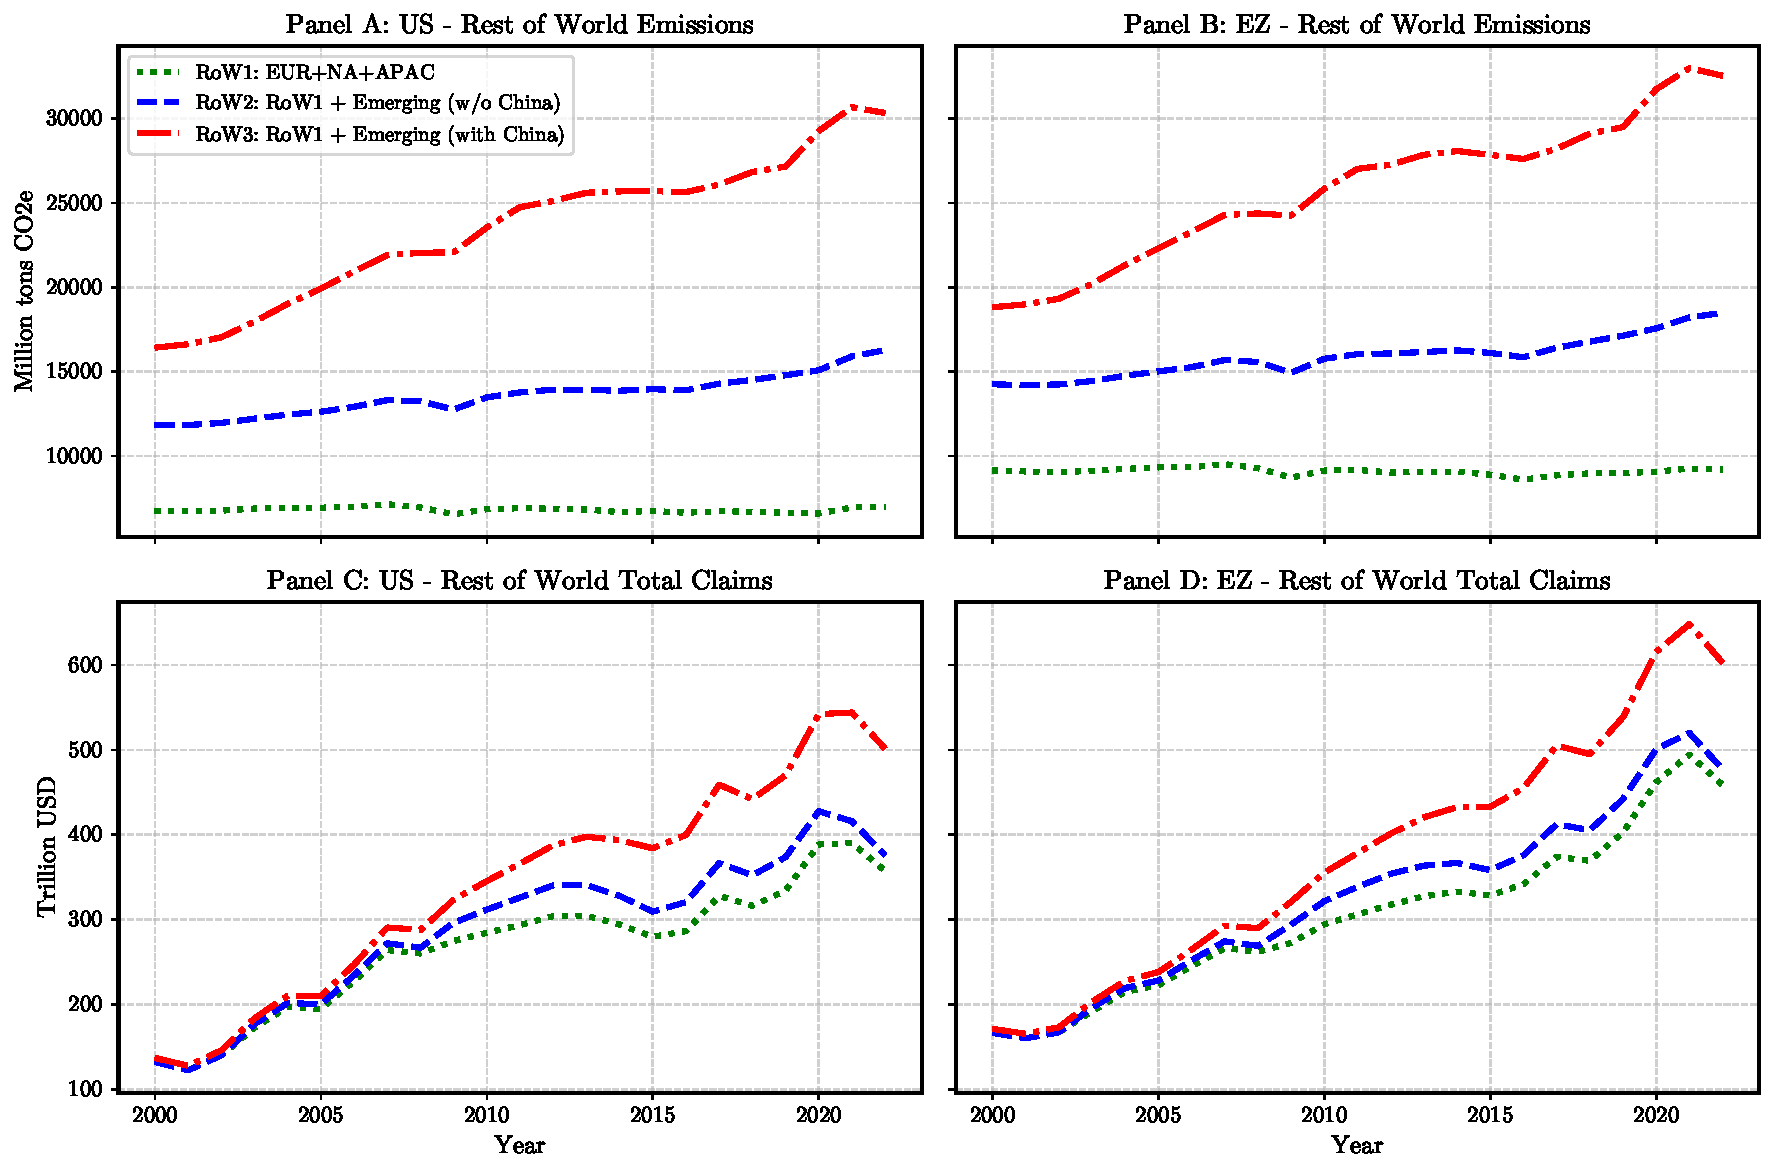
\includegraphics[width=1\textwidth]{Figures/Decomposition_RoW.pdf}
    \caption{Decomposition of Carbon Intensity for the Rest of World}
\end{figure}
\chapter{Financed Emissions by Financial Institutions}
\label{Appendix E:FE_by_FI}

\begin{figure}[h]
    \centering
    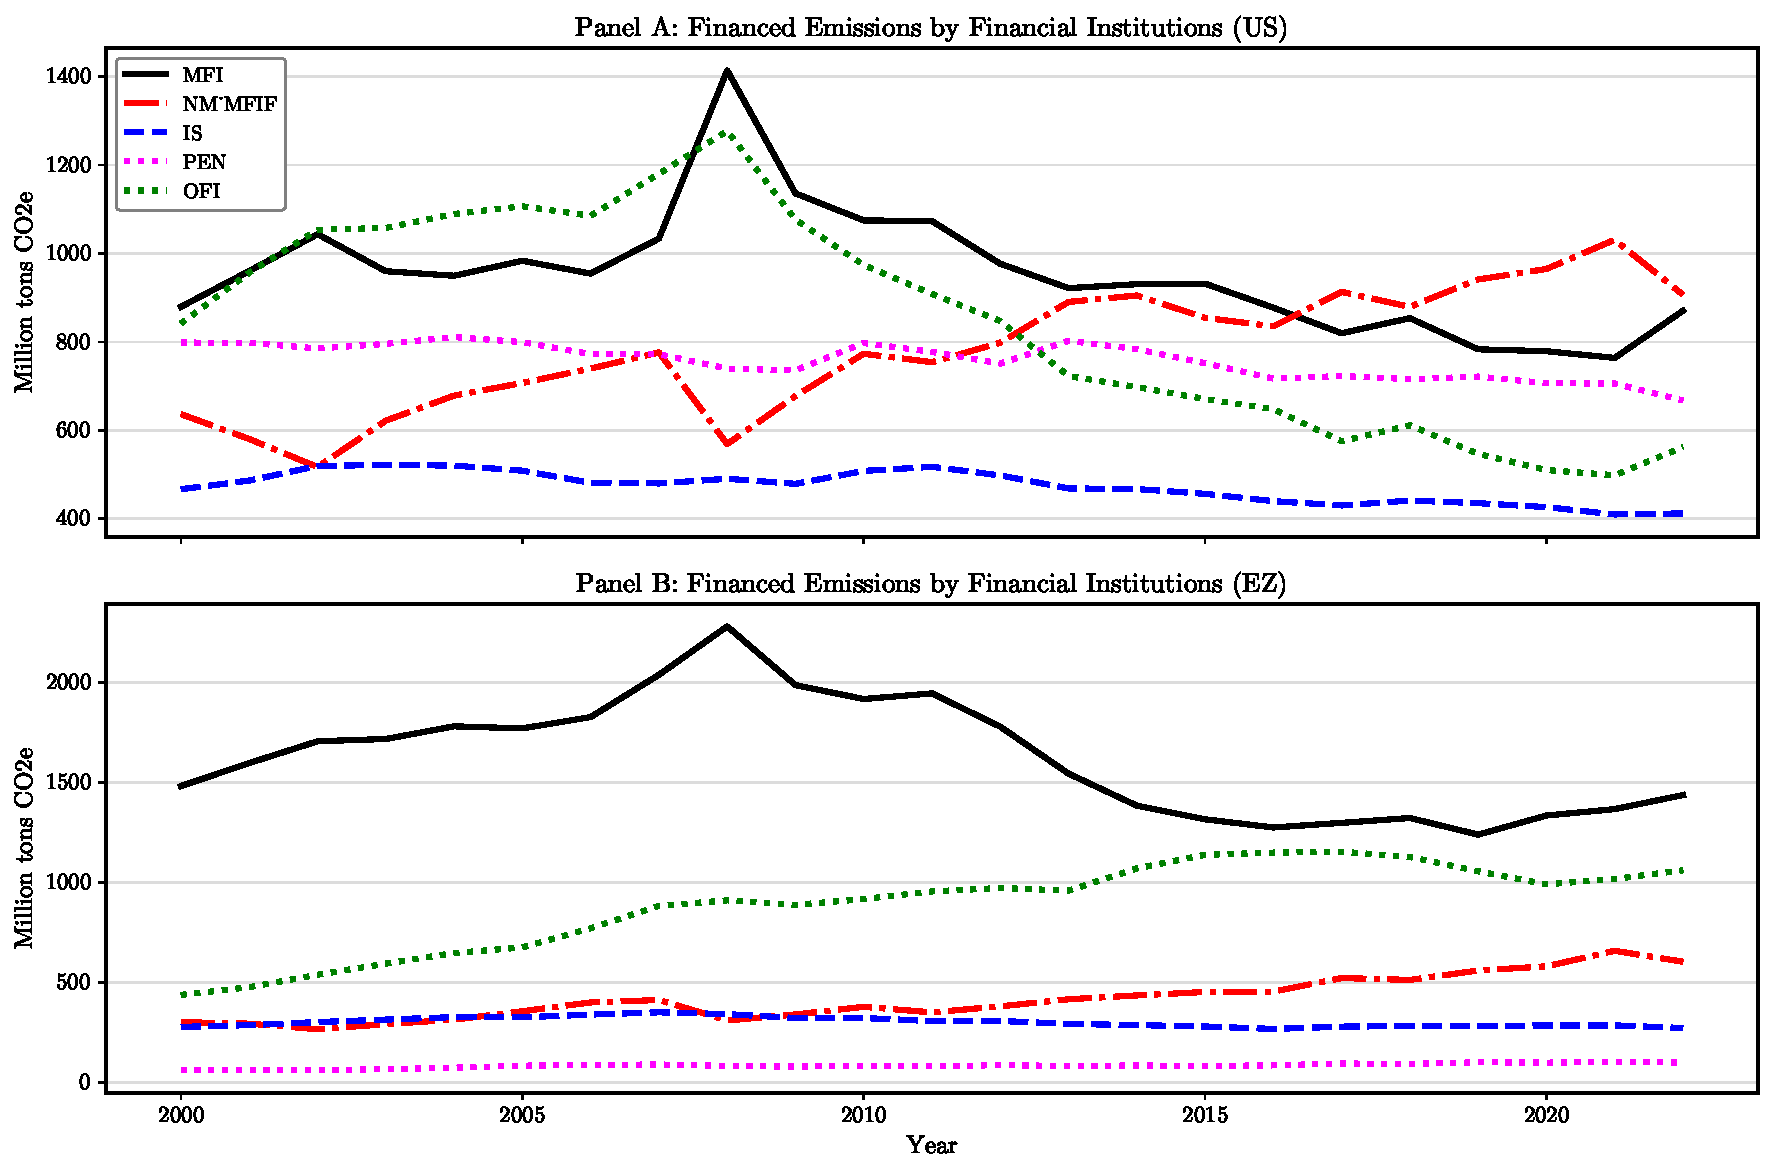
\includegraphics[width=1\textwidth]{Figures/FE_by_Institutions_RoW2.pdf}
    \caption{Total financed emissions by financial institutions group (RoW2)}
\end{figure}

\begin{figure}[t!]
    \centering
    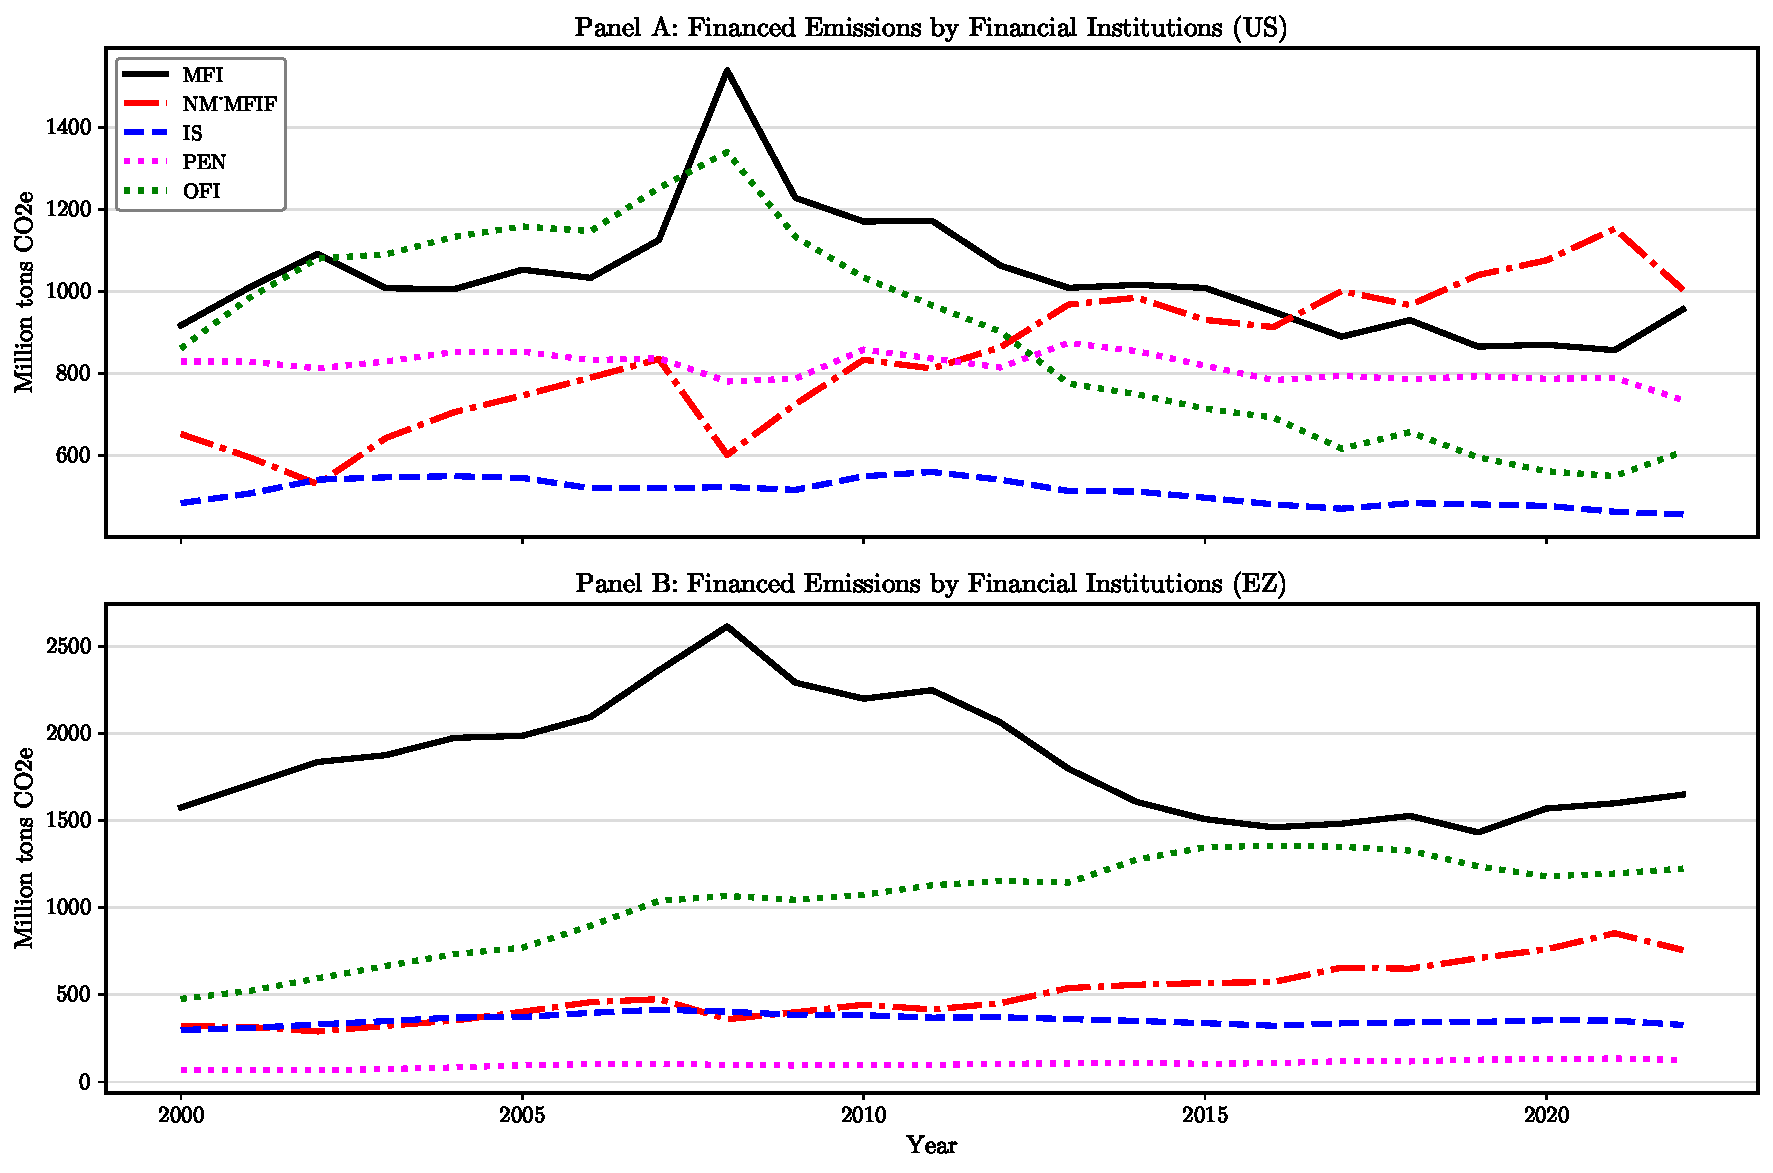
\includegraphics[width=1\textwidth]{Figures/FE_by_Institutions_RoW3.pdf}
    \caption{Total financed emissions by financial institutions group (RoW3)}
\end{figure}
%----------------------------------------------------------------------------------------
%	BIBLIOGRAPHY
%----------------------------------------------------------------------------------------

\printbibliography

%----------------------------------------------------------------------------------------

\end{document}  
